\documentclass[a4paper,11pt]{ujreport}
\usepackage{style/nislab,style/thesis}

%----------------------------------------------------------------------
% 修論・卒論 執筆 注意事項
%----------------------------------------------------------------------
% 章立て
% * 章のなかに節が1つだけの場合は,節を立てる必要がありません.節の中に小節が1つだけの場合も同様です.
% * つまり,chapterの中には,sectionは2つ以上あるべきで,sectionが1つの場合は,そのsectionは不要で,chapter直下に内容を記述すべきです.
% * 論文の概要と「はじめに」(イントロダクション)は異なるものです.概要は結果も含めた論文全体の概要であり,「はじめに」は解決すべき問題を明示するための背景情報および論文でその問題をどう取り扱うかの導入について記載するものです.

% 背景と目的
%   * 最初に「背景と目的」を書くのが一般的かと思いますが,「背景と目的」は論文の概要ではありません.
%   * なぜ,この研究をする必要があるのか,一般的な世間の状況と,研究を行う必要性を書くことになります.
%   * 単に今までに無かったので作ったではダメです(例:AとBをつなぐシステムが無かったので作りました)
%   * 世の中でその問題にどう取り組んでいるかは,一般には「関連研究」のところで説明します.
%   * 一般的な背景情報はこの章にまとめてください(本文中に一般的背景情報を書くべきではありません)
%   * また,この章では,論文の技術的な内容や結果を書く必要がありません.なぜなら「背景と目的」だからです.
%   * 一方,論文の「概要」は,研究結果および論文の結論まで含めて書くべきです.

% 提案方式の説明
%   * 問題に関して,自分の解決方法を説明します.
%   * 問題そのものを簡単に理解できない場合は,問題についても詳解が必要です.
%   * 問題をどうやって解決するかを手順を追って解説します.
%   * 複数の問題が関連している場合は問題を分離して説明します.
%   * 自分の解決方法が従来とどこが違いどう工夫しているかを明記する必要があります.

% 評価
%   * 自分の解決方法を問題点に適応してどういう結果が得られたかについて説明をします.
%   * 従来技術や手法と比較してどこがどうよくなったかを示します.
%   * どのような環境で比較したかを説明する必要があります.
%   * 定量的に以前(関連研究)と比べてこうよくなったと説明できればベターです.

% 考察
%   * なるべくなら考察を章で分けて下さい.提案方式に関する「評価」に関して記載する章があるのが一般的かと思いますが,「考察」の章では,従来技術や関連研究と比較して,評価結果がどうであったかを考察して下さい.

% まとめ (★特に修論の場合の注意点★)
%   * 800 字から1000字ぐらいでまとめてください.
%   * 背景,解決すべき問題点,提案内容,結果,考察,研究の意義などを含めて記載してください.
%   * 結果については,過去形(・・・実施した.・・・評価した.・・・確認した.など)で記載してください.

% 参考文献
%   * 勉強した書籍を列挙するものではありません.
%   * 本文中に引用した技術などを記載するものです.
%   * 参考文献の番号は,必ず本文中の引用場所を示します.(本文中に引用の番号がない参考文献は存在しません)

% 表現
%   * 自分が出した結果に対して「・・・と考えられる」や「・・・と言える」は使わないで下さい.
%   * 関連研究などの他人の出した結論に対しては OK.
%   * 一般的に断言できない場合は,条件を設定して「・・・という条件においては,・・・である」と断定してください.
%   * 文中に副詞を用いる場合は,その副詞が本当に必要かどうかをよく考えて下さい.
%   * 略語は,論文の最初に登場したところで何の略語であるかを記載して下さい.
%   * 文中は定量的な表現を使って下さい.大きい/小さい,長い/短い,速い/遅い,など.何をもって大きいと言えるのか,などを考えて下さい.

% ページ数
%   * 修論は本文が20ページ以内.図を含めて20ページを越えても問題ありません.
%   * 卒論は20ページ以上で記載して下さい.
%   * 出版物になりますので,権利関係が明確になっていない場合,同志社大学あるいはその関係者以外に著作権のある図の利用は不可です.

% 提出
%   * 必ず,締切の前日までに事務に提出してください.締切の当日に(交通機関の遅延,病気などの一般的には正当な理由があっても)遅れた場合は受理されません.

%----------------------------------------------------------------------
% 表紙用
%----------------------------------------------------------------------
\type{2}  % 1:卒業論文 2:修士論文
\title{未知領域探査のための複数ドローンを利用した \\動的な三次元環境地図生成によるAR 可視化}  % 日本語タイトル
\etitle{Multiple Drones-Based AR Visualization \\with Dynamic Environmental Maps for Unknown Area Exploration}  % 英語タイトル
\author{竹内 一真 / Kazuma Takeuchi}  % 著者
\date{2023年1月25日}  % 日付
\advisor{佐藤 健哉 教授}  % 指導教員
\university{同志社大学大学院} % 大学名
\department{理工学研究科 情報工学専攻} % 専攻
\lab{ネットワーク情報システム研究室}  % 研究室
\entryyear{2021}  % 入学年度
\studentnumber{0145}  % 学生番号

%----------------------------------------------------------------------
% 変更不要
%----------------------------------------------------------------------
\begin{document}
\maketitle
\clearpage

%----------------------------------------------------------------------
% 概要
%----------------------------------------------------------------------
% 卒業論文は日本語(200~400文字),修士論文は英語(200~300単語)で書く.
% 改行は不要
%----------------------------------------------------------------------
% 自動運転車両に搭載されたセンサ情報を通信し,安全性と効率化を目指した協調型自動運転の研究が行われている.さらに,共有したセンサ情報を管理してアプリケーションを実行するための情報通信プラットフォームであるダイナミックマップシステムが検討されている.しかし,インターネット上のクラウドで動作するダイナミックマップシステムでは,通信遅延やスケーラビリティに関しての懸念がある.そこで,地理的に分散配置したエッジサーバを利用することで,アプリケーションを効率的に実行可能になると考えられる.また,移動する車両に対してエッジサーバとの接続や,エッジサーバ間での連携が課題となる.本研究では,車両が走行する道路上のエリアを「LID」として分割し,それに基づいてエッジサーバを割り当てたダイナミックマップシステムを開発した.さらに,車両周辺の交通環境に基づいてデータの送信間隔を調整する優先度制御機能や,複数の通信方式を併用しデータをフィルタリングする複数経路通信機能を実装した.車両の走行シミュレーションを行い,従来システムと比較して,車両が送信先となるエッジサーバを意識せずにデータ送信し,低遅延に通信し,効率的にアプリケーションが実行できることを示した.管理する車両台数に応じた処理遅延やスループットを評価することで,スケーラビリティが向上することを示した.

\begin{abstract}
% 近年,小型ドローンは機体が小さいことから,人間が入れないような狭小空間での利用が検討されており,将来的には狭小空間の未知領域探査への応用が期待されている.
% しかし,狭小空間では遮蔽物が多いため,操縦者の死角領域内にてドローンを飛行させる必要があり,十分に周辺を監視することができず,安全なドローン操縦は困難である.
% また,狭小空間の未知領域探査では,走行する環境情報がなく,一台のドローンのみで探査を行うには多くの時間を必要とするため,バッテリー上限が短いドローンでは,探査を完了することが困難である.
% そのため,複数ドローンを利用することで,各ドローンの走行時間を減少させ,探査効率を向上させる必要がある.
% そこで,操縦者とドローンの間に遮蔽物が存在し,ドローンを視認できない狭小空間に対してARを利用することで,操縦を支援する方式を検討する.
% 本稿では,各ドローンがリアルタイムで飛行環境をマッピングし生成された三次元環境地図をもとに,ARを用いて操縦者の死角領域内に存在するドローンと周辺環境を可視化する方式を提案し,従来の操縦とARを用いた方式を比較し,評価した.
% その結果,提案方式では平均操縦時間,平均衝突警告回数が減少し,操縦の自信度が向上したため,探査効率,安全性の向上を示した.

In recent years, small drones have been examined to play an active role in narrow spaces where humans cannot enter due to the small size of the spaces, and are expected to be applied to the exploration of unknown areas in confined spaces in the future.
However, it is difficult to control the drone within the pilot’s blind spot where there are many obstructions in a small space. 
In addition, in the exploration of unknown areas in confined spaces, it is difficult for a drone with a short battery limit to complete the exploration because there is no information on the environment in which the drone is traveling and a large amount of time is required for only one drone to perform the exploration.
Therefore, it is necessary to use multiple drones to reduce the running time of each drone and improve the efficiency of exploration.
Augmented Reality can address these issues for the environments where the drone cannot be seen due to the presence of obstructions between the operator and the drone. 
In this paper, we propose a method to visualize drones in the operator's blind spot area and the surrounding environment using AR, based on a 3D environmental map generated by mapping the flight environment in real time for each drone, and compare and evaluate the conventional control and AR-based methods.
As a result, the proposed method reduced the average maneuvering time and the average number of collision warnings, and increased the confidence level of the pilot, thereby improving exploration efficiency and safety.

\end{abstract}

% キーワードを3つ設定する
% 卒業論文は日本語,修士論文は英語
\addkeywords{augmented reality}{visualization}{unknown area exploration}

%----------------------------------------------------------------------
% 変更不要
%----------------------------------------------------------------------
\footnote[0]{本論文に掲載の製品名・会社名等は,一般にそれぞれの会社の商標,または登録商標である.}
\footnote[0]{なお,本文中では\texttrademark ・ \textregistered 等のマークは特に明記していない.}

%----------------------------------------------------------------------
% 変更不要
%----------------------------------------------------------------------
% ページ番号をギリシャ数字にする
\pagenumbering{roman}

% 目次を1ページから始めるために表紙を0ページにする
\setcounter{page}{0}

% 目次を作成
\tableofcontents

% 改ページ
\clearpage

% 以降,ページ番号をアラビア数字で振り直す
\pagenumbering{arabic}

%----------------------------------------------------------------------
% はじめに
%----------------------------------------------------------------------
\chapter{はじめに}
\label{chap:Introduction}

% ******************** Section ********************
\section{背景・課題}
\label{sec:Background}

近年,多方面でのドローンを活用した事業が登場しており,インフラ点検や災害調査など,応用分野を拡大しながら,ドローン用途は急速に成長し,熟練された操縦者に限らず,より多くの人がドローンを使用する機会が増加している\cite{article-drone01}\cite{article-drone02}.
中でも小型ドローンの特徴である機体の大きさを活かして,人間が入れないような狭い空間での活躍の場も増加しており\cite{article-drone04}\cite{article-drone05},将来的には狭小空間の未知領域探査への応用が期待されている.
しかし,狭小空間での小型ドローン飛行は,遮蔽物が多く,操縦者は遮られた視点からの操縦を必要とする\cite{article-drone03}.
本論文では,狭小空間により,操縦者と小型ドローンの間に遮蔽物があり,小型ドローンを視認できない環境を「死角領域」と定義する.
死角領域内の小型ドローン操縦では,小型ドローンを視認できない中,衝突することなく,安全に操縦する技術が求められる.

\par
ドローンの操縦に関する技術の提案は複数あるが\cite{article-drone07}\cite{article-ar01}\cite{book-drone05},ドローンを操縦する際の視点の呼び方について統一した定義がないため,本論文ではドローン操縦視点を次のように定義し,各操縦視点の概要を\figref{fig:01_viewpoint}に示す.
\begin{itemize}
  \item 一人称視点\mbox{}:ドローンを操縦する操縦者の視点.操縦者の視点から視認できる範囲のみを頼りに操縦を行う.
  \item 二人称視点\mbox{}:ドローンに搭載されたオンボードカメラの視点.操縦者はドローンから送られる空撮した映像を基に,ドローン中心の視点での操縦を行う.
  本研究では死角領域内での操縦を前提としているため,操縦者はドローンから送られる空撮した映像のみを頼りに操縦を行う.
  \item 三人称視点\mbox{}:ドローンの視点でもなく,操縦者の視点でもなく,それ以外の環境に設置されたカメラの視点.ドローンのカメラ映像や,実物のドローンを視認することなく操縦を行う.
\end{itemize}
\par
一人称視点操縦の場合では,操縦者はドローン周辺の状況を視認し,把握することができ,また,ドローンの実際の高さや位置を正確に把握することができる\cite{book-drone02}.
しかし,一人称視点による操縦では,操縦者から見えるドローンまでの距離感が掴めないため\cite{article-ar01}\cite{article-ar02},ドローン周辺の障害物へ衝突する恐れがある.
大型ドローンでは,自律飛行や障害物回避などの機能が実現されているが,センサ搭載制限のある小型ドローンでは,障害物回避の支援がないことが多く,衝突の危険性がある.
また,障害物回避を搭載していても,狭小空間では障害物回避が行えない場面が多く存在する\cite{article-drone12}.
\par
二人称視点操縦の場合では,操縦者はオンボードカメラ搭載ドローンを使用することで,ドローンから送られる空撮した映像を元に操縦が可能となる\cite{article-drone08}.実際の現実空間を映像として見ながら操縦できるため,現実のドローンを視認することなく,狭小空間を探索することができる\cite{book-drone02}.
しかし,カメラが前方しか写さないことにより\cite{article-drone09},カメラ映像のみを頼りに操縦する必要がある.カメラ映像だけでは,空間認識能力が低下し\cite{article-drone10},状況認識が不十分となるため\cite{article-drone11}\cite{book-drone03},狭小空間のように狭く,障害物が多いような環境では,操縦は困難である.
\par
三人称視点操縦の場合では,主に遠隔操作を行う必要がある環境下において検討され,操縦するドローンとは別に二台目のドローンを追尾し飛行させ,その周辺を撮影することによる多視点でのドローン操縦が実現されている\cite{book-drone05}.
しかし,障害物回避が行えない場面が多い狭小空間では,二台目のドローンを自在に移動できず,三人称視点操縦を実現することは困難である.
そこでVR(仮想現実,Virtual Reality)を利用することで,操縦者の物理的な視点とは独立した多視点を追加・移動させることにより,ドローン操縦性を向上することができる\cite{book-drone04}.
しかし,VRでは仮想空間に没入した状態でドローン操縦を行うため\cite{article-drone13},操縦者が完全に仮想環境へ没入し,現実環境で起こった変化などを目視することができず危険である.

\par
また,狭小空間の未知領域探査では,走行する環境情報がないため,探査完了までに時間がかかることが想定される\cite{book-multi01}\cite{book-multi02}.
しかし,ドローンはバッテリー上限が短く,短時間での効率的な探査を必要とする中で\cite{article-drone14}\cite{article-drone15}\cite{article-drone16},一台のドローンのみで探査を行うには多くの時間を要すため,未知領域探査を中断する恐れがある.

そこで,1台のドローンではなく複数台のドローンを使用することによる,各ドローンの走行時間の減少,探査効率の向上が期待されている.
しかし,複数のドローンによる未知領域探査の利点を活かすためには,各ドローンが協調的に動作する必要がある.
\figref{fig:01_collision},\figref{fig:01_efficient}に示すように,環境中のドローンの数が多ければ多いほど,衝突のリスクは高くなり,また,各ドローンが走行した環境を把握していなければ,探査領域の重複も考えられ,探査効率を低下させる恐れがある.

\begin{figure}[!tb]
  \centering
  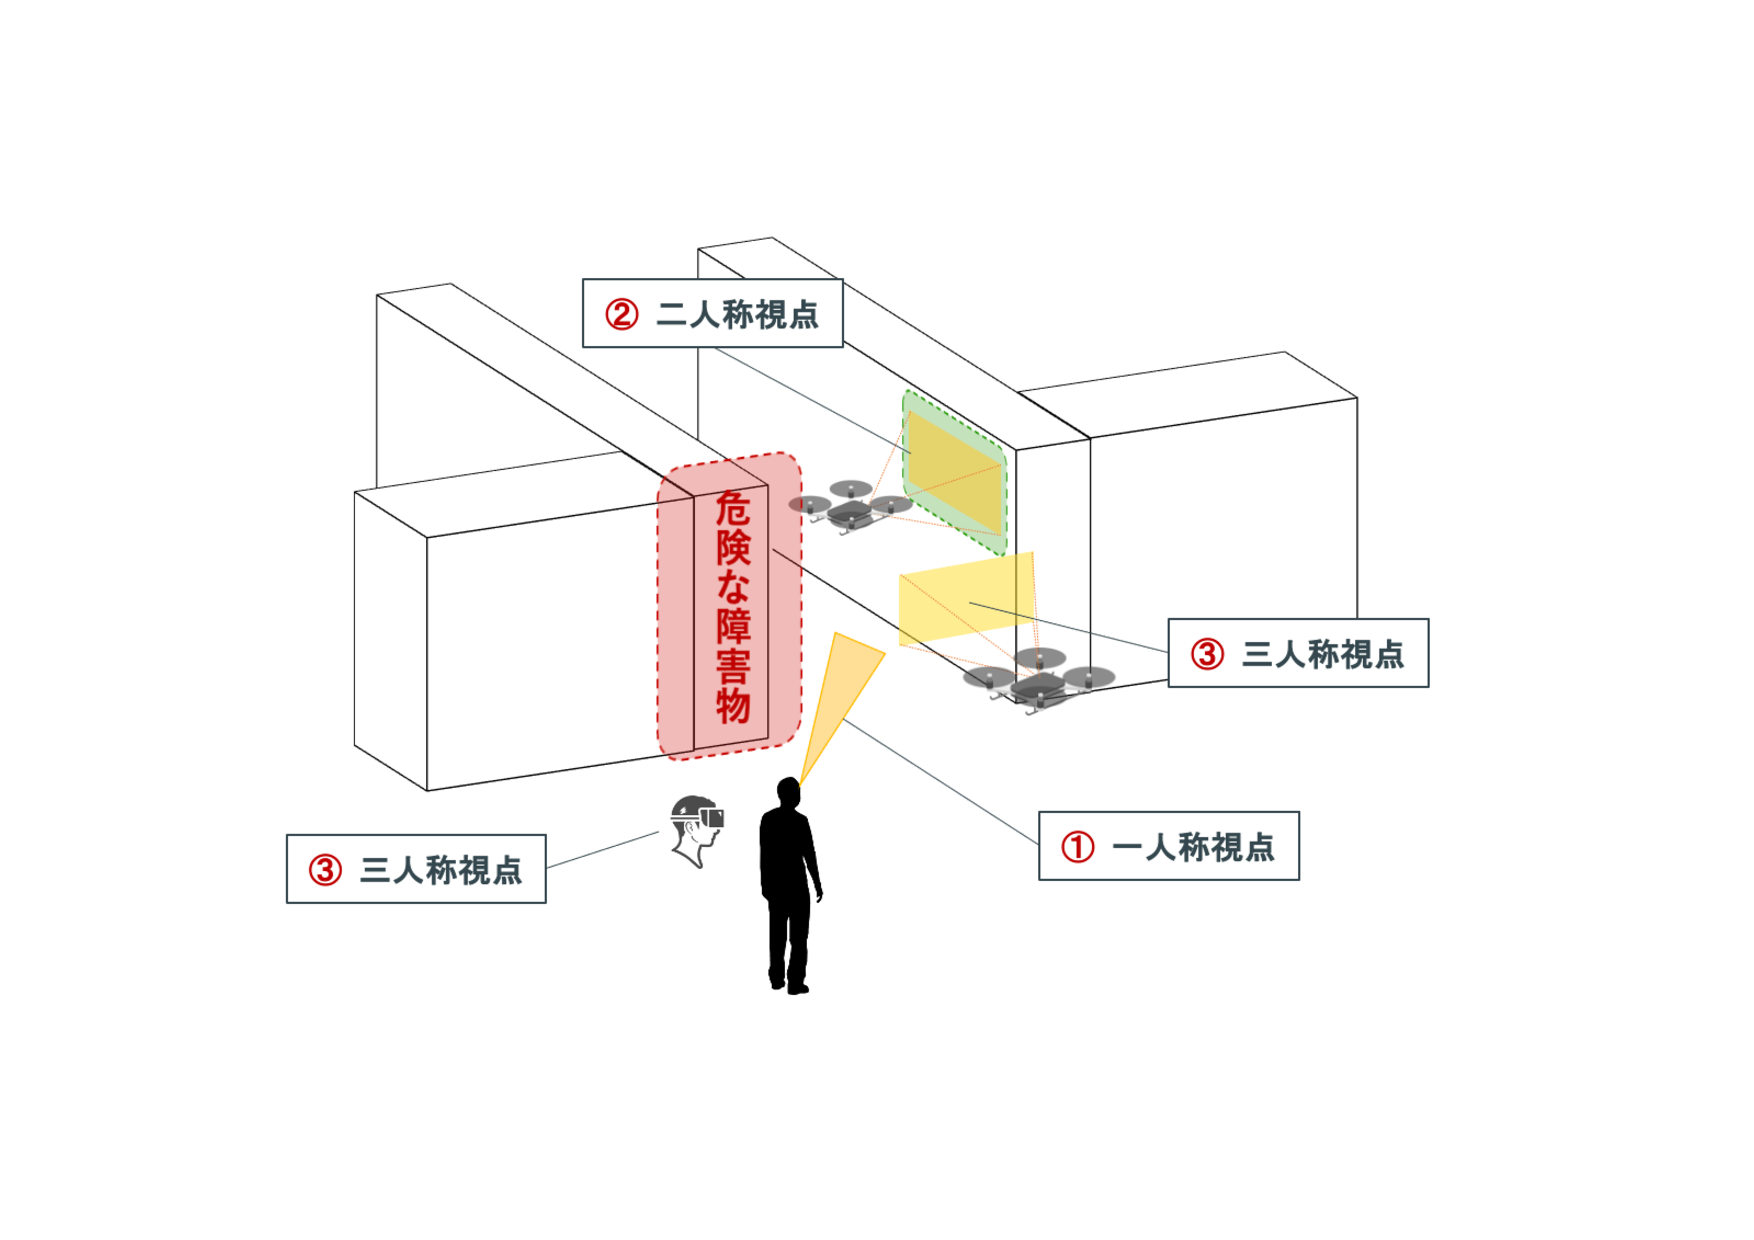
\includegraphics[width=\linewidth]{img/01_viewpoint.pdf}
  \caption{ドローン操縦視点}
  \label{fig:01_viewpoint}
\end{figure}

\begin{figure}[!tb]
  \centering
  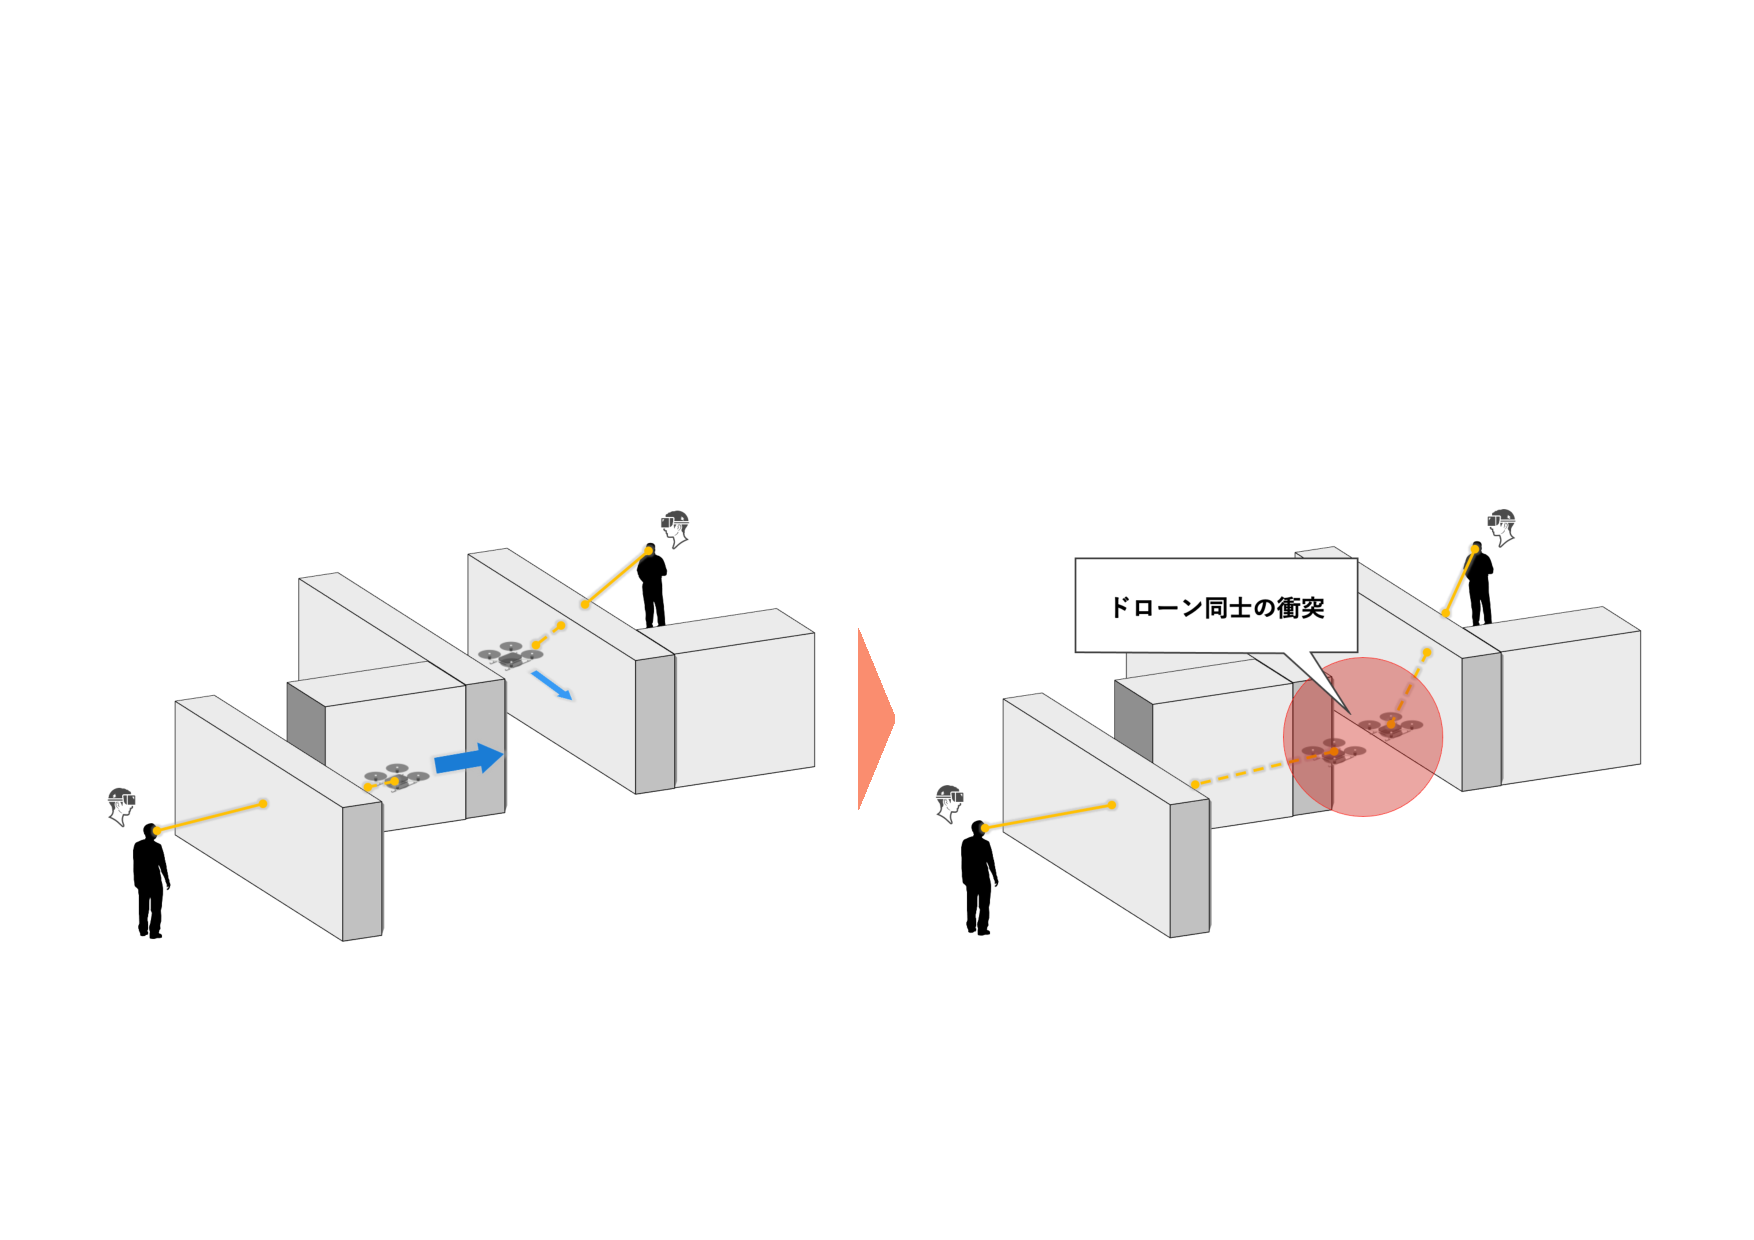
\includegraphics[width=\linewidth]{img/01_collision.pdf}
  \caption{複数ドローン混在時における衝突危険性}
  \label{fig:01_collision}
\end{figure}

\begin{figure}[!tb]
  \centering
  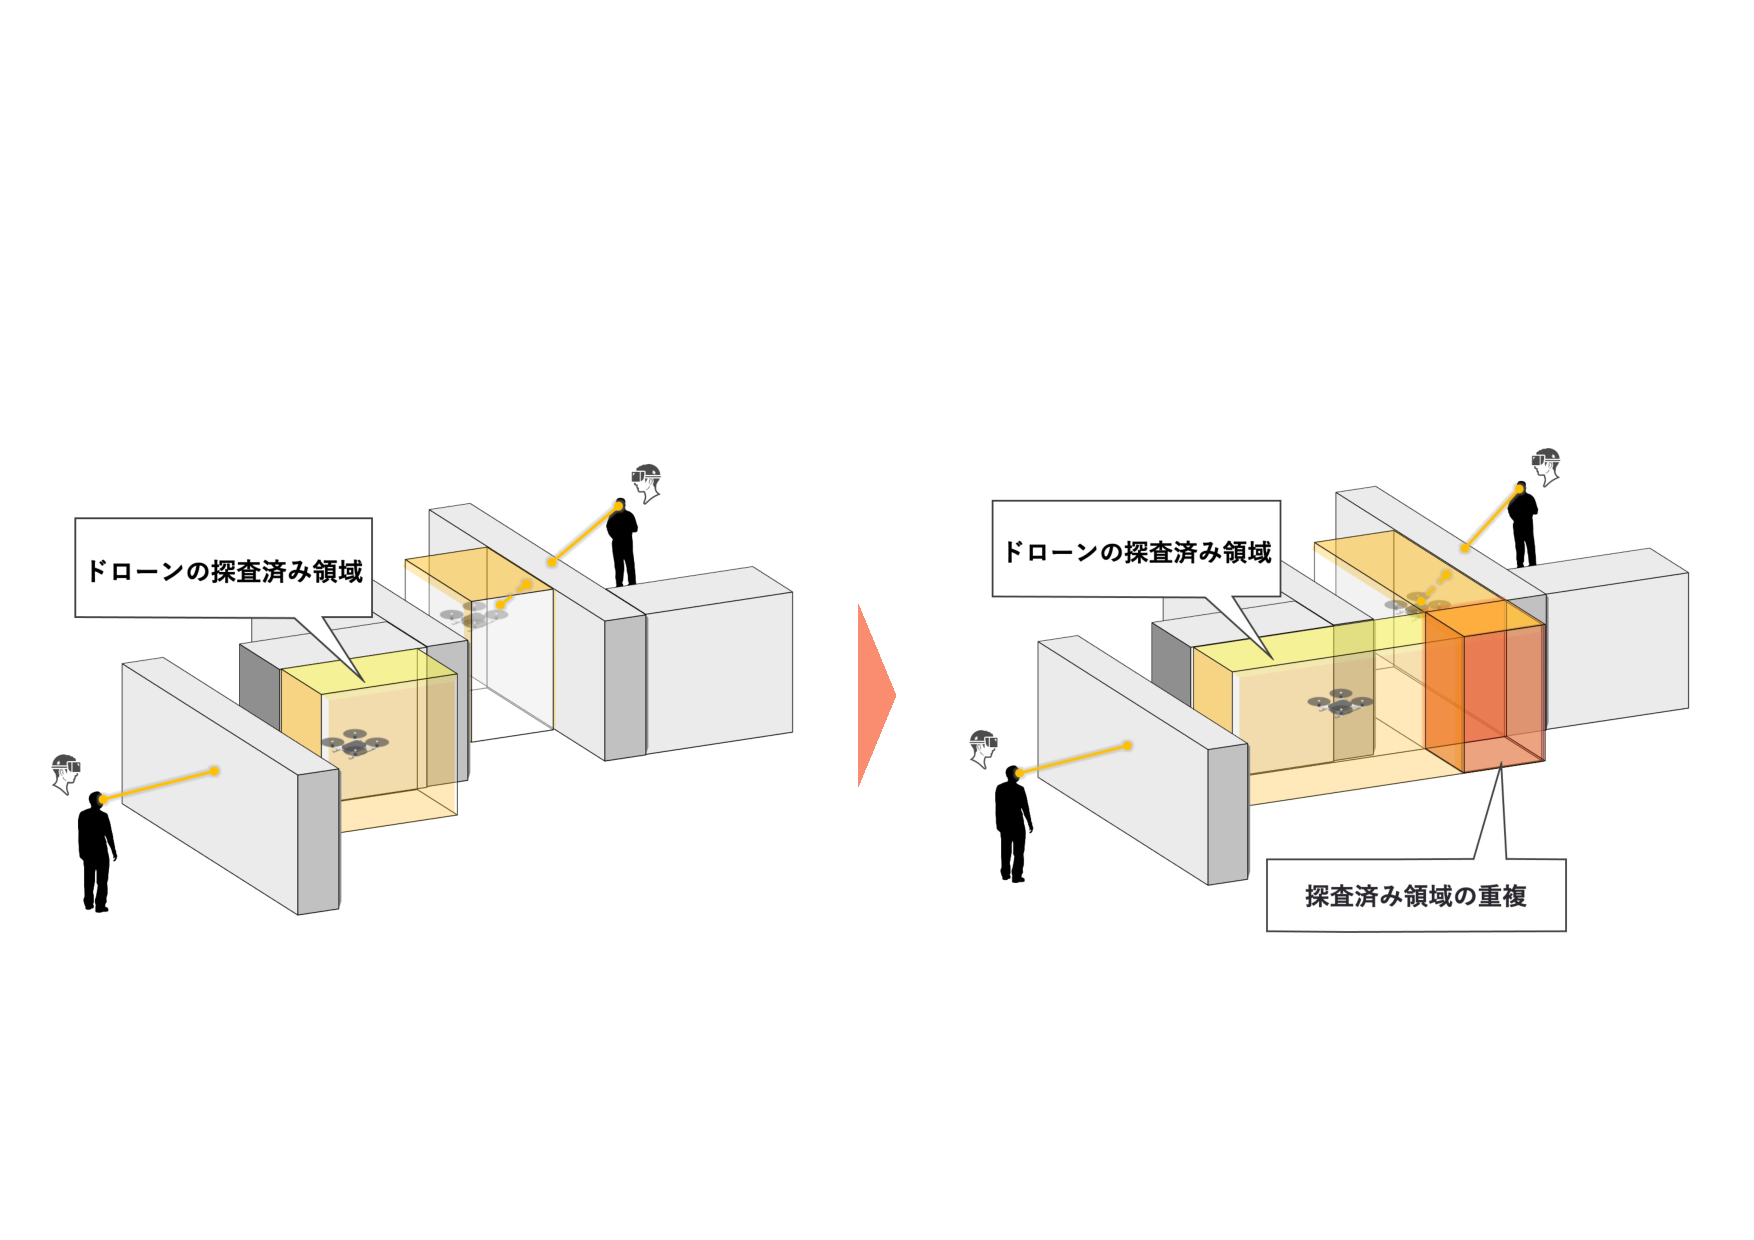
\includegraphics[width=\linewidth]{img/01_efficient.pdf}
  \caption{複数ドローン混在時における探査効率の低下}
  \label{fig:01_efficient}
\end{figure}


% ******************** Section ********************
\section{目的}
\label{sec:Purpose}

本研究では,狭小空間による死角領域内において,未知領域探査へ投入するドローン数の増加に伴う,探査効率の問題を軽減するため,
各ドローンがSLAM(Simultaneous Localization and Mapping)を用いて取得したセンサ情報を統合した上で,AR(拡張現実,Augmented Reality)により操縦者の死角領域内を可視化する方式を提案する.
これにより,複数人が協調的にドローンの連携を図り,複数ドローンによる衝突危険性の低減させた上で,探査効率を向上させる方式を実現し,その有効性を評価する.

% ******************** Section ********************
\section{本論文の構成}

第\ref{chap:RelatedWorks}章では,複数ドローンを用いた未知領域探査,狭小空間による死角領域内でのドローン操縦の関連研究について説明する.
第\ref{chap:ProposedMethod}章では,本章で述べた問題点を解決する提案方式の概要や探査効率,安全性の向上のための複数の機能について説明する.
第\ref{chap:Development}章では,提案方式を実現するための実装方法や実験環境について述べる.
第\ref{chap:Experiment}章では,提案方式の有効性の評価のための実験方法とその評価結果について述べる.
第\ref{chap:Discussion}章では,実験によって得られた結果に対して考察を行う.
第\ref{chap:Conclusion}章では,本論文のまとめを述べる.\par

%----------------------------------------------------------------------
% 関連研究
%----------------------------------------------------------------------
\chapter{関連研究}
\label{chap:RelatedWorks}

\begin{figure}[tb]
  \centering
  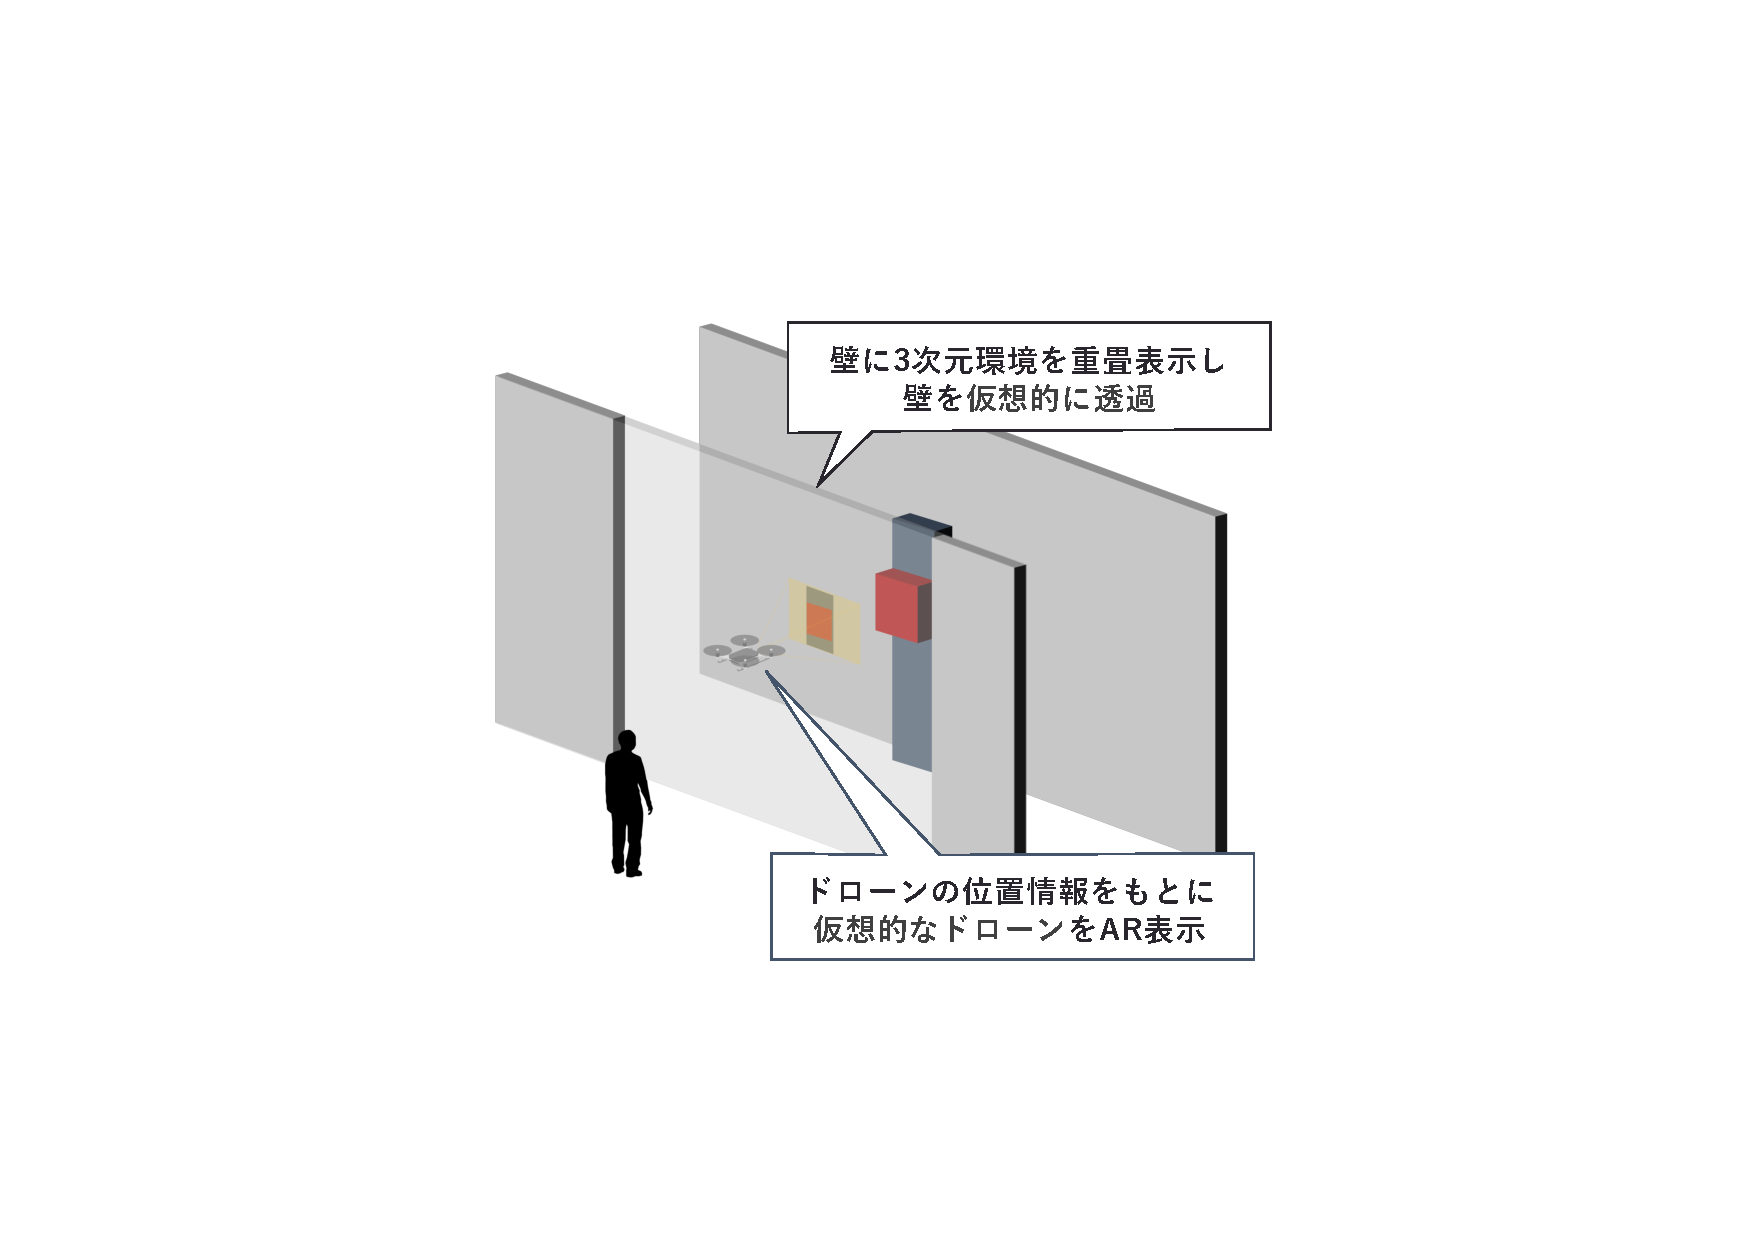
\includegraphics[width=0.7\linewidth]{img/02_relation.pdf}
  \caption{狭小空間での一人称視点によるドローン操縦手法}
  \label{fig:02_relation}
\end{figure}

% ******************** Section ********************
\section{未知領域探査へのドローンの有用性}
\label{sec:UnknownArea}
Mahdouiらの研究\cite{book-multi03}では,小型で機動性に優れたドローンを複数台飛行させ,協調的な自律飛行をシステムを用いて,屋外の未知領域探査を行うためのアルゴリズムを提案している.
複数ドローンを用いることによるドローン同士の衝突や,探査範囲の重複を防ぐため,各ドローンが異なる領域を同時に探査する必要がある.
そこで,各ドローン間で通信を行い,どこが既に探索されたか,どこが未だ探索されていないかを共有し,適切な区間を探査するための手法を提案している.
結果として,実験環境中のドローン数が多いほど,それぞれのドローンに要求される探索率が低くなり,探査にかかる時間の短縮に成功することができた.

しかし,ドローンの数が多いほど,各ドローンの移動時間,移動距離が直線的に少なくなるわけではなく,ドローン台数が増えるほど,衝突の危険性や探査効率の低下を引き起こすことが問題点として挙げられる.
また,ドローンが自律飛行できることを前提にしているため,屋内のような狭小空間に対して適応することができない.
そのため,実際に操縦者がドローン操縦を行う際に,複数ドローン間が通信することによる探査効率への影響が不明瞭であるため,
未知領域探査への有効性を調査する必要がある.


%2.2
\section{狭小空間におけるドローン操縦手法}
\label{sec:NarrowSpace}

Liuらの研究\cite{book-ar04}では,三人称視点のドローン操縦において,操縦者前方の床やテーブル上にドローン周辺の三次元環境をAR表示することにより,自律飛行するドローンに適切な目的地を提供することを可能にするARインタフェースを提案している.
結果として,操縦者はドローン周辺の三次元環境に没入することができ,飛行空間の探索に成功することができた.
しかし,自律飛行することのできない狭小空間では,操縦者の意図を伝えて飛行させることができない.また,デスクトップPCインタフェースと比較評価した結果,ARインタフェースは操作精度を犠牲にしていた.
そのため,タスク完了までに時間がかかる問題を抱えており,ドローン操縦性を低減する可能性が高い.

Eratらの研究\cite{article-ar05}では,狭小空間による死角領域内の,一人称視点でのドローン操縦手法を提案している.\figref{fig:02_relation}が示すように,事前に空間マッピングにて用意した三次元環境を用いて,閉鎖環境をAR可視化している.
結果として,ドローン視点での二人称視点操縦と比べ,一人称視点でのドローン操縦手法では,タスク完了までの操縦時間が半分以下となっている.

しかし,未知領域でのドローン操縦において,事前に三次元環境地図を用意することは困難なため,
実際の未知領域探査において,ドローンが一からマッピング,自己位置推定などを行う環境でも同じ効果を発揮できるのか示されていない.
また,関連研究では一台のドローンのみを想定していたが,複数ドローンを適応する場合,自身が操縦するドローン以外の飛行しているドローンを発見することが困難である.
その上,自身が操縦するドローン以外の飛行しているドローンが,これからどこを探査しようとしているのか,どこまで探査したのかを把握できないため,探査範囲の重複を引き起こすことが想定される.
そのため,各ドローンの位置情報や探査領域を把握できないことによる,複数ドローン間の衝突危険性や探査済み領域の再探査を低減させる,各ドローンのセンサ情報を共有できる操縦方式が必要である.


%----------------------------------------------------------------------
% 提案方式
%----------------------------------------------------------------------
\chapter{提案方式}
\label{chap:ProposedMethod}

% ******************** Section ********************
\section{概要}
\label{sec:ProposedOutline}

本研究では,ARを用いて死角領域内の空間認識を提供し,複数ドローンのセンサ情報を統合することにより,未知領域探査の効率性,ドローン操縦の安全性を向上させる.
\par
\figref{fig:03_enviroment}の環境におけるドローン操縦を想定しており,飛行するドローンと同じ人数の操縦者が,遮蔽物に阻まれた先に飛行している各ドローンを操縦することを前提としている.
提案方式では,操縦者はARHMD(Augmented Reality Head-Mounted Display)を装着しており,死角領域内および飛行しているドローンをARによって可視化することにより,一人称視点でのドローン操縦を実現している.
ドローン操縦環境には,もう一台ドローンが飛行していることを想定しているため,自身のドローンの位置情報,ドローンのカメラ映像をもとに取得した点群データおよび,二台目のドローンの位置情報,二台目のドローンが取得した点群データを相互に共有している.
操縦者は,受け取った位置情報をもとに,ARによる仮想ドローンを表示し,点群データをもとに三次元環境地図を表示することにより,視覚支援を受け取っている.
提案方式の概要を\figref{fig:03_outline}に示す.


% \begin{figure}[tb]
%   \centering
%   \begin{minipage}{0.4\linewidth}
%     \centering
%     \includegraphics[width=0.9\linewidth]{img/edgeserver_send_using_ack.pdf}
%     \caption{ACKを利用した再送機能}
%     \label{fig:edgeserver_ack_data}
%   \end{minipage}
%   \begin{minipage}{0.5\linewidth}
%     \centering
%     \includegraphics[width=0.9\linewidth]{img/transfer_ack_between_edgeserver.pdf}
%     \caption{ACKのエッジサーバ間転送}
%     \label{fig:edgeserver_ack_transfer}
%   \end{minipage}
% \end{figure}

\begin{figure}[tb]
  \centering
  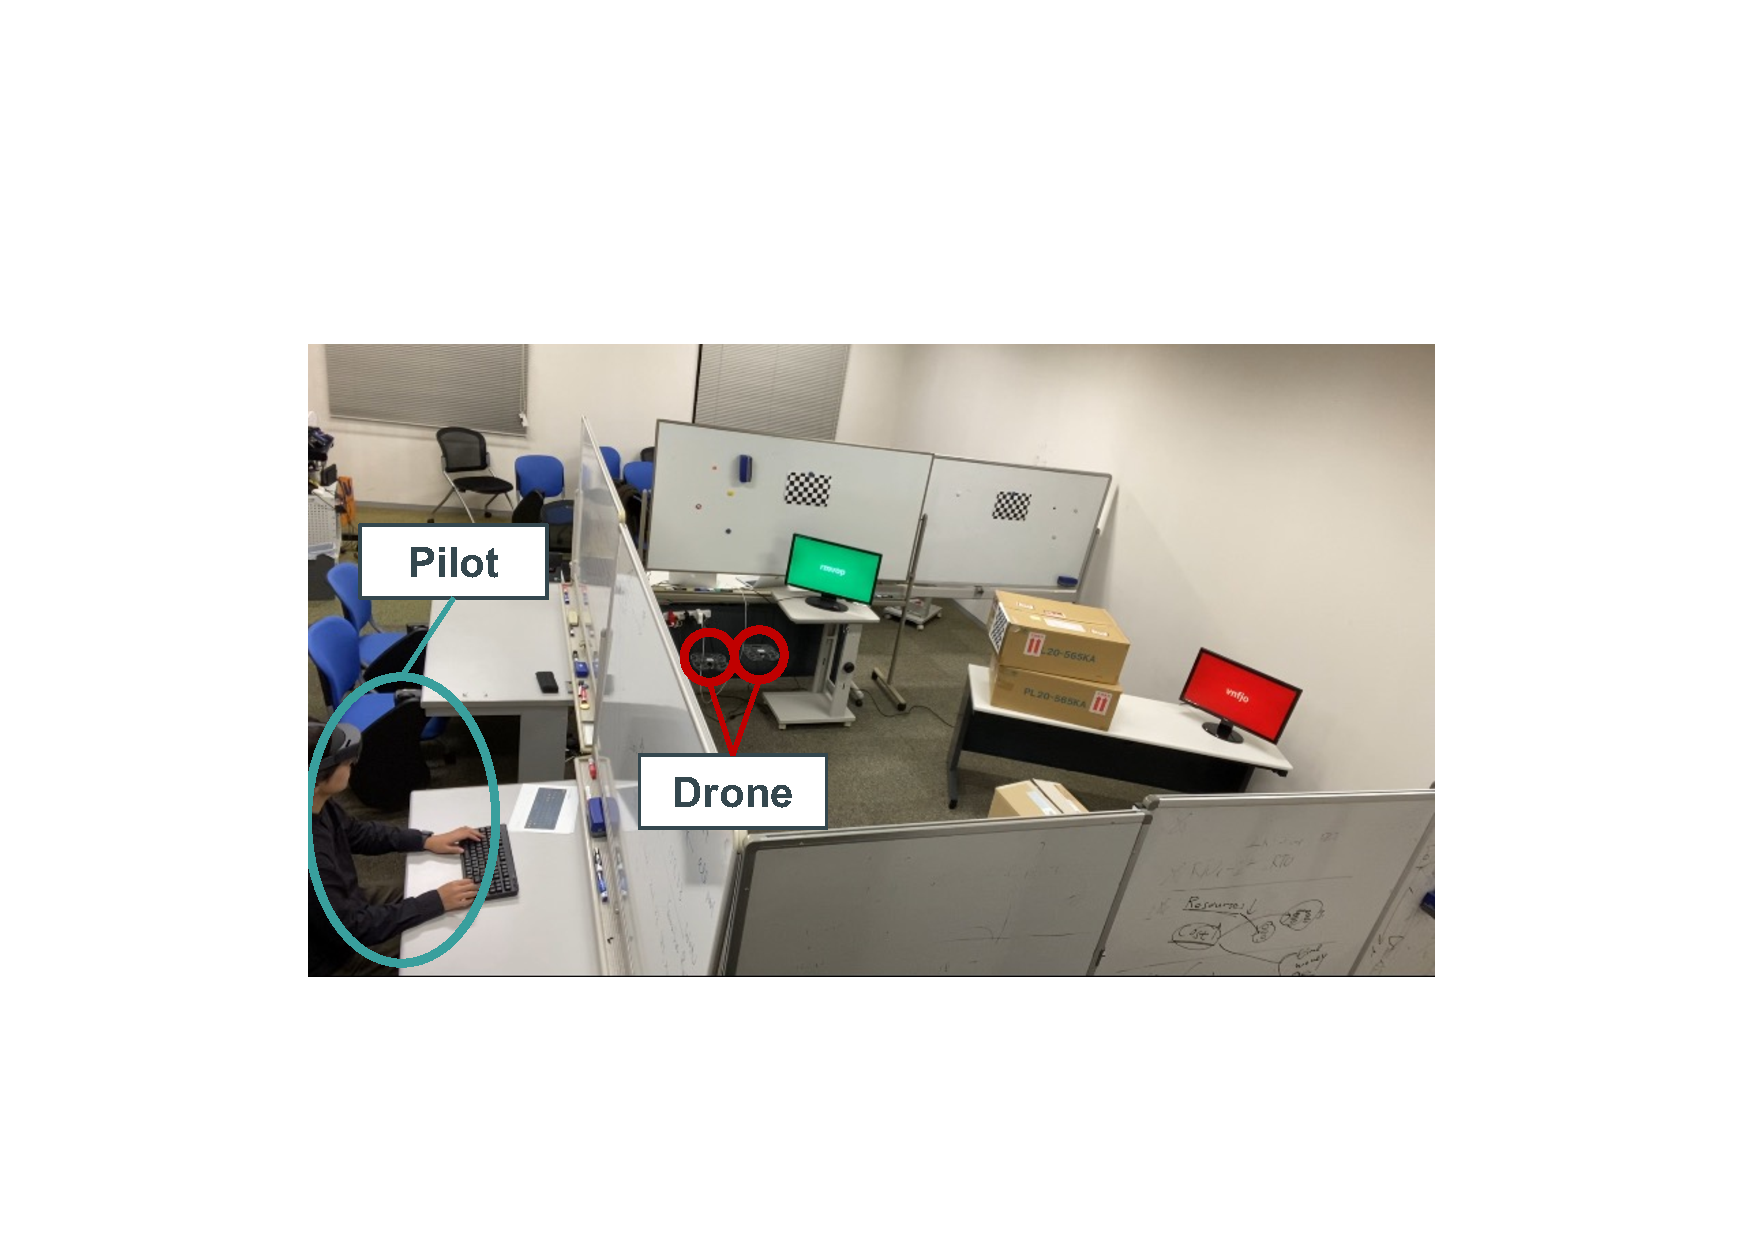
\includegraphics[width=0.7\linewidth]{img/03_enviroment.pdf}
  \caption{未知領域でのドローン操縦環境}
  \label{fig:03_enviroment}
\end{figure}

\section{死角領域内に位置する遮蔽物のAR可視化}
\label{sec:ARvisualize}
本提案方式では,ドローンと操縦者の間に遮蔽物が存在する場合,ドローンが飛行している場所が操縦者にとっての死角領域となる.
死角領域が存在すると判断したとき,三次元環境地図における遮蔽物を透過した上で,現実環境に重畳表示することで,仮想的に死角領域の空間認識を提供する.
操縦者は,死角領域内を飛行するドローンを視認することはできないが,ARによって仮想のドローンと,ドローン周辺の三次元環境を視認することができる.

しかし,本提案方式ではドローンのカメラ映像に対してリアルタイムに画像処理を行い,マッピングを行なっているため,初めから三次元環境地図全てを取得することはできない.
そのため,ドローン自身で周囲を見渡しながら走行することによって,ドローン周辺がどのような環境なのかを徐々に把握することとなる.
つまり,初めからドローン周辺の三次元環境地図を取得することはできず,ドローン前方に位置する物体のみを認識することができ,辺りを見渡していくことによって,カメラ映像に新たに移った物体を
三次元環境地図として取得することができる.

この際に,\figref{fig:03_pointcloud}に示すように,ドローンのカメラ映像をもとにvSLAM(visual SLAM)を実行することによって,ドローン周辺の環境を点群データとして取得している.
点群データは,コンピュータで扱う点の集合であり,三次元空間上の物体形状を,その表面上の観測点の直交座標 $(x,y,z)$ の集合という形式で表現する.
ここで取得した点群データが多数の点 $n$ の三次元座標として出力され,メッシュ処理を行うことで,三次元環境を取得する.

% 提案方式の遮蔽物を透過した画像を添付
\begin{figure}[!tb]
  \centering
  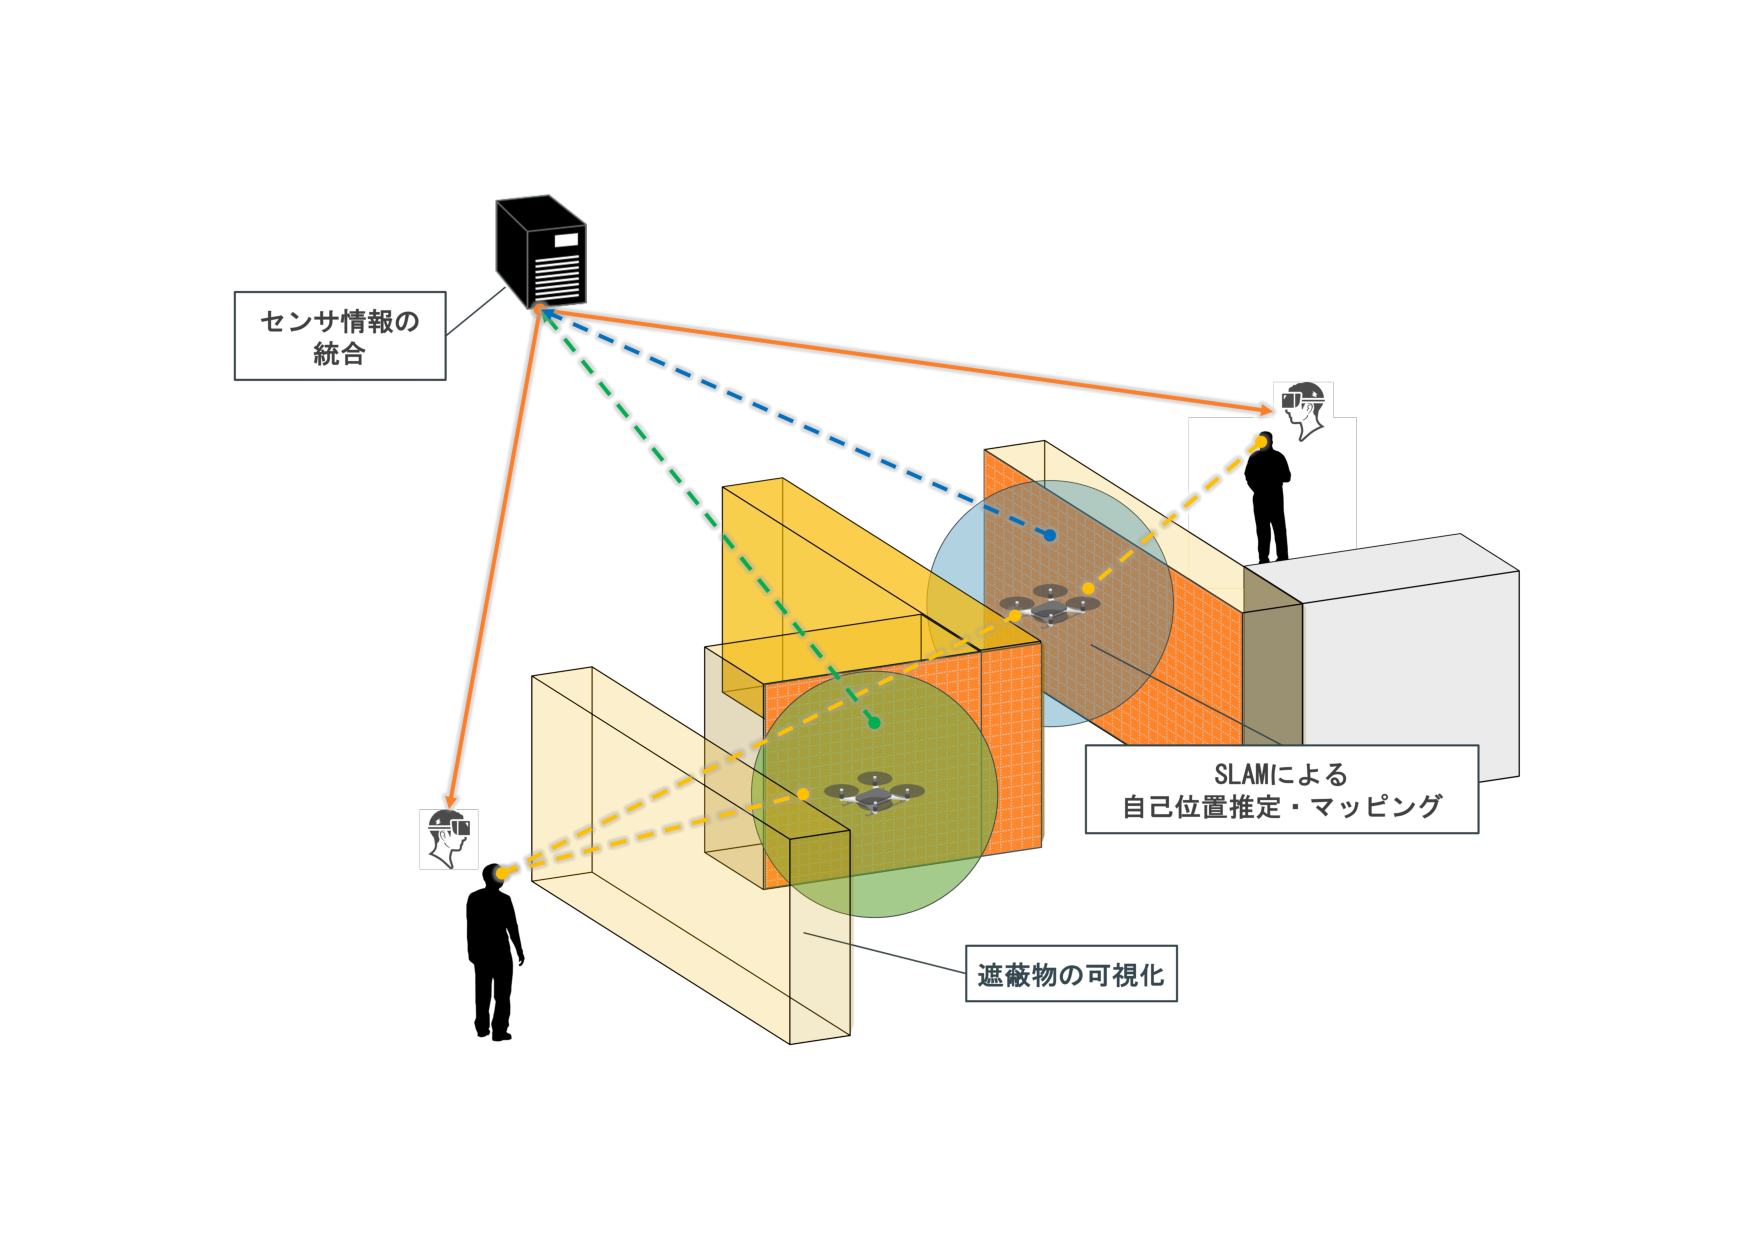
\includegraphics[width=\linewidth]{img/03_outline.pdf}
  \caption{提案方式の概要}
  \label{fig:03_outline}
\end{figure}

しかし,vSLAMによって取得する点群データは,どのvSLAMを使用するのか,また,どのようなカメラを使用するのかによって,大きく左右される.
そのため,使用する技術,カメラに左右されずに提案方式の有効性を確認する必要性がある.
そこで,\figref{fig:03_restore}に示すように,事前に三次元環境地図を取得した上で,取得した点群データ座標付近に存在する三次元環境地図を復元することで,
リアルタイムでのマッピングを再現している.
% つまり,ARHMDでは,ドローンのカメラ映像をもとに取得した点群データを利用し,段階的に三次元環境地図を復元していき,操縦者へ視覚支援を行うため,ドローン周辺の環境が徐々に可視化されていく.
事前に取得した三次元環境地図もSLAMにより取得しているものであるため,本提案方式のみ優れた視覚支援が行われていることはない.



% 図形を利用して表現
\begin{figure}[!tb]
  \centering
  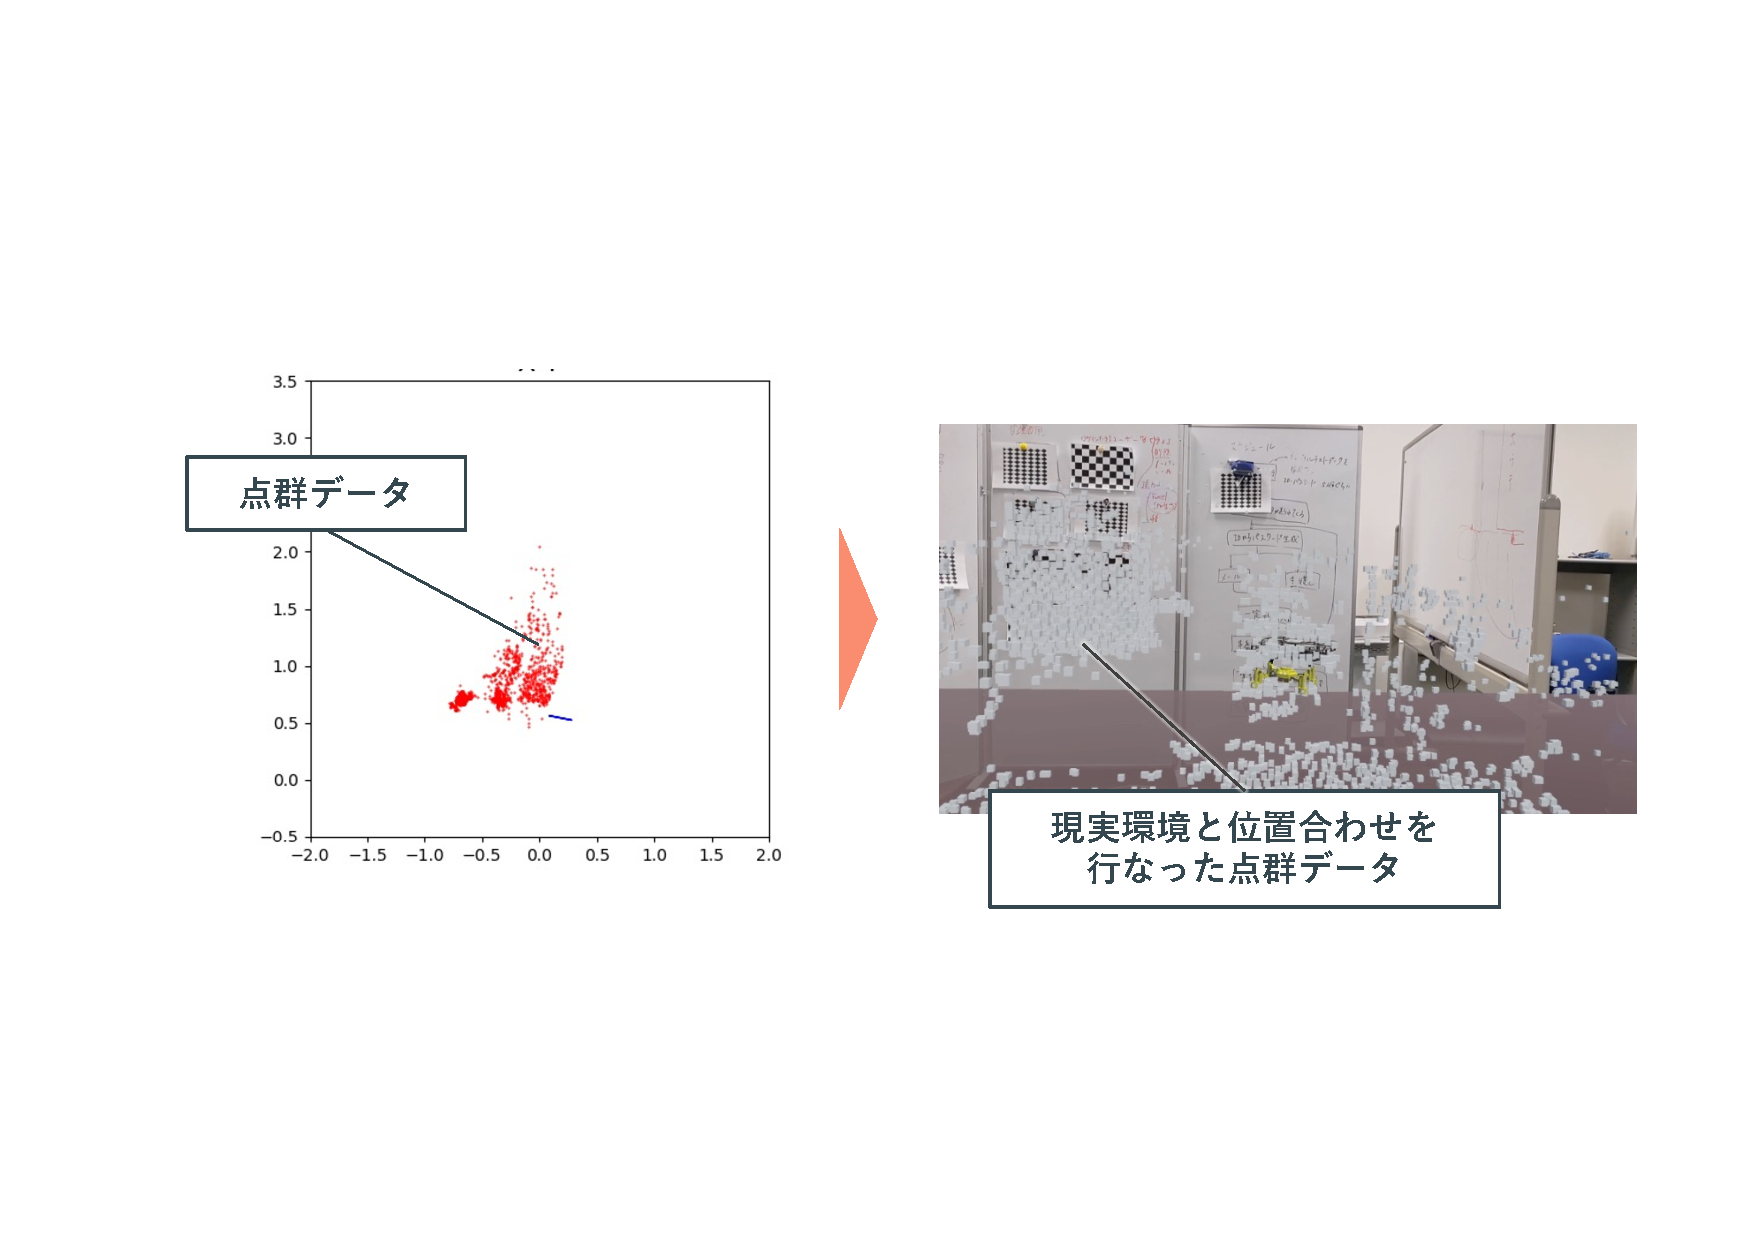
\includegraphics[width=0.9\linewidth]{img/03_pointcloud.pdf}
  \caption{vSLAMにより取得した点群データ}
  \label{fig:03_pointcloud}
\end{figure}

\begin{figure}[!tb]
  \centering
  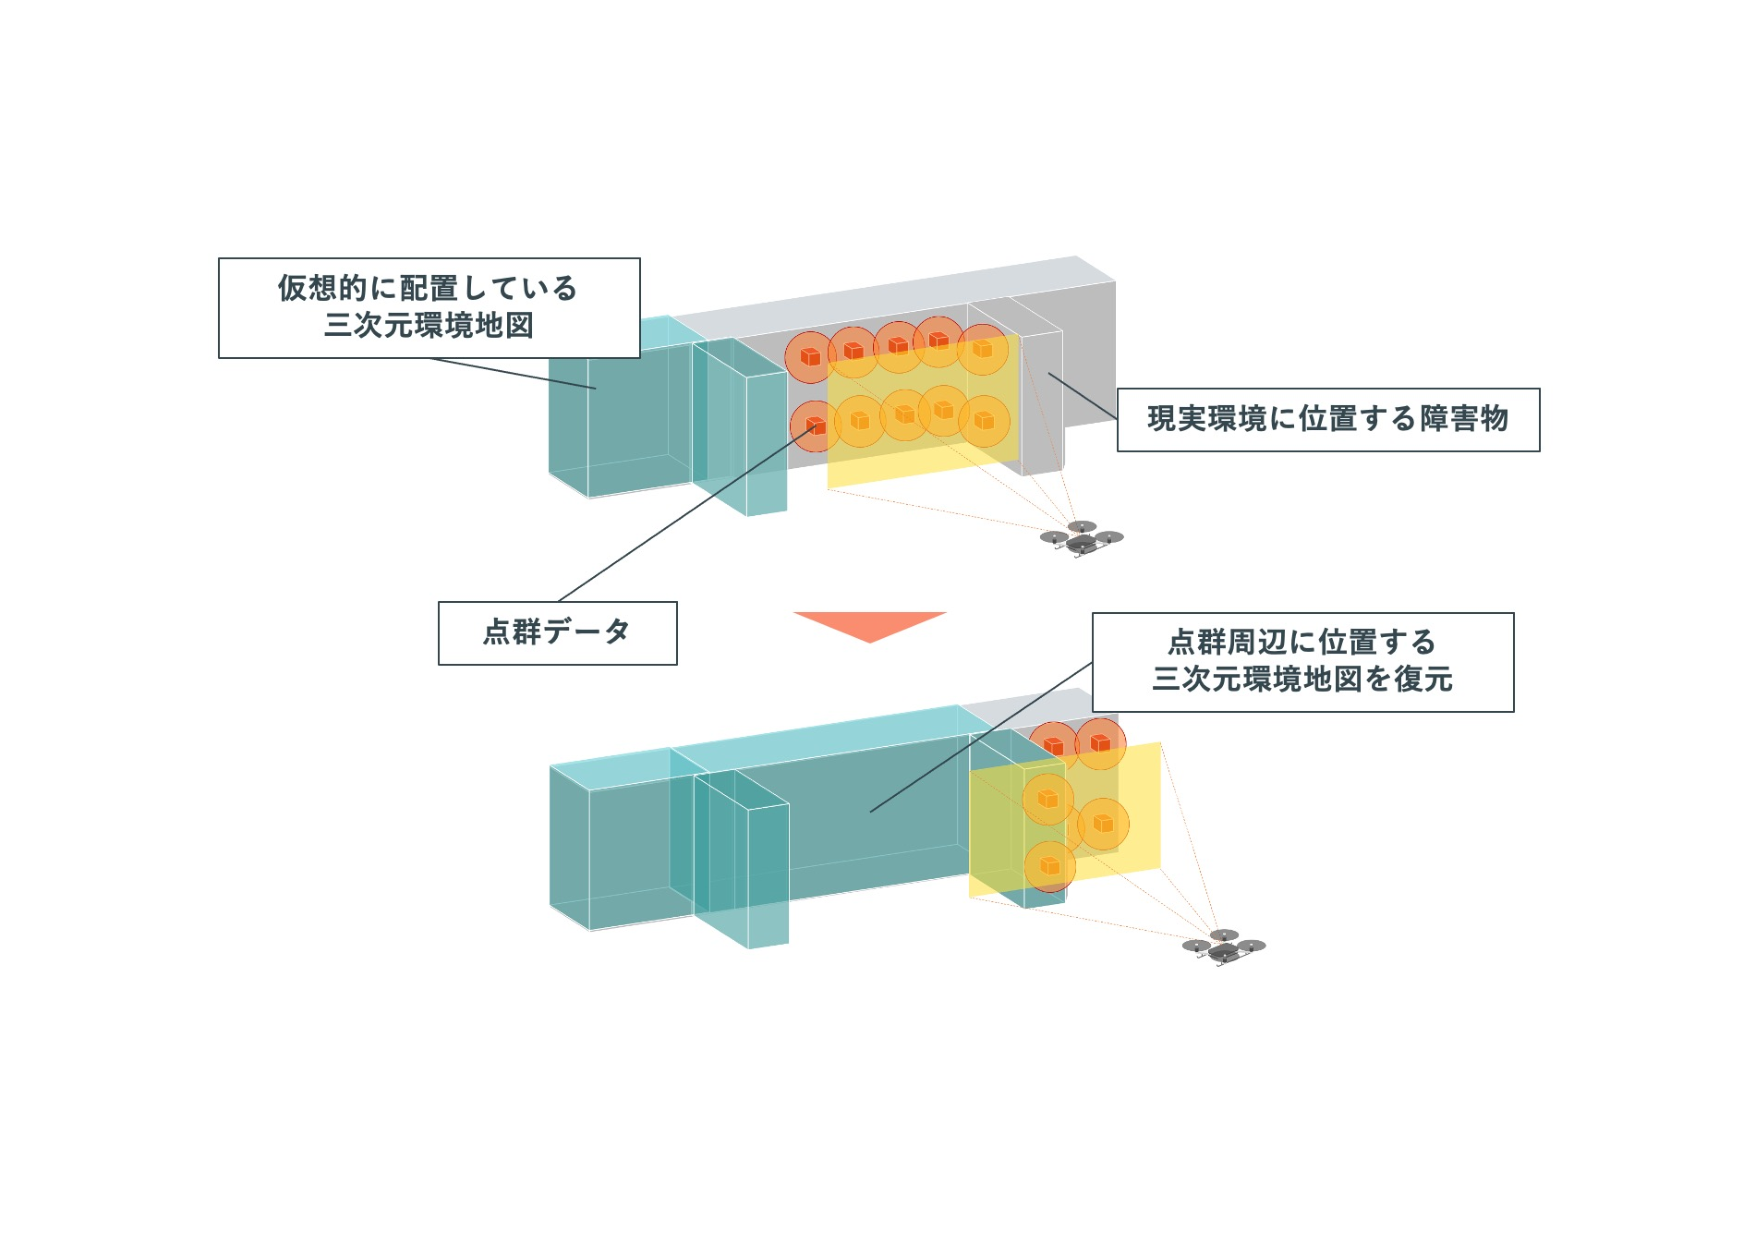
\includegraphics[width=0.9\linewidth]{img/03_restore.pdf}
  \caption{三次元環境地図の復元}
  \label{fig:03_restore}
\end{figure}

% 各ローカル座標を管理している図を表現
\begin{figure}[bt]
  \centering
  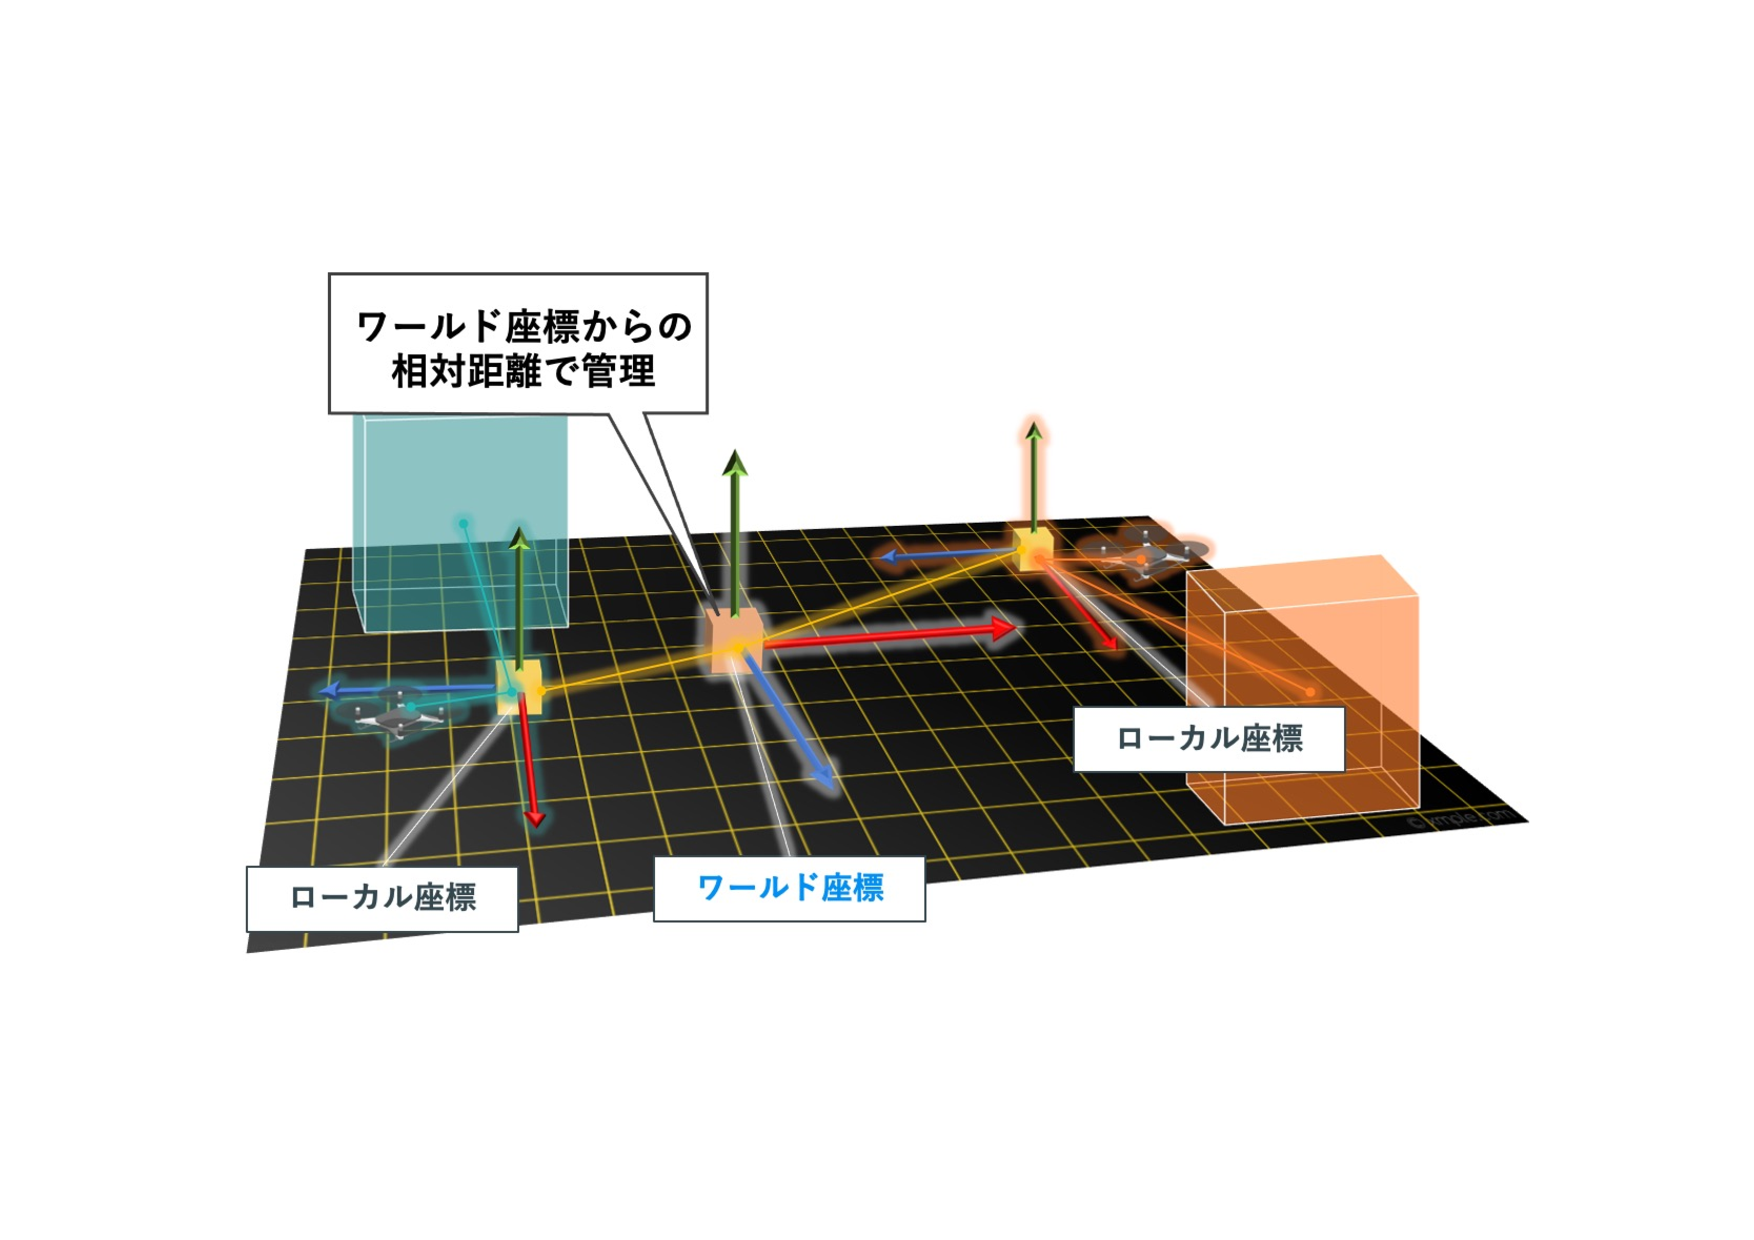
\includegraphics[width=0.9\linewidth]{img/03_cordinate.pdf}
  \caption{ワールド座標での一元管理}
  \label{fig:03_cordinate}
\end{figure}

\section{複数ドローンのセンサ情報統合}
\label{sec:SensorIntegration}

複数ドローンのセンサ情報を統合することにより,各ドローンの位置情報,点群データ,また画像処理をうまく行えているかの判定を操縦者の装着しているARHMDに送信している.
一方で,ARHMDでは仮想表示しているドローンが近傍の障害物へ衝突しそうな場合に,衝突判定のデータをサーバへ送信している.
これにより,操縦者にとっての死角領域内がどのような環境になっているのか,また,複数ドローンが死角領域内のどこを飛行しているのか,ドローン周辺に危険な障害物が位置していないかを把握することができる.

ドローンは自身が取得した点群データを送信するが,ドローンの位置情報や点群データはドローンが起動した位置座標を中心に管理されており,位置情報や点群データの座標は中心座標からの相対座標として扱われている.
しかし,複数ドローンを扱う際には,扱うドローンの台数分の中身座標が存在するため,ARHMDが受信する各ドローンの位置情報,点群データは個々で独立してしまう.
そのため,ARHMDで受信した各種データを,実際の現実環境と位置合わせを行うことができず,現実のドローンと同じ位置に仮想ドローンを配置することもできない.
その上,ドローンから送信される位置情報と現実環境との位置合わせを行えないことにより,
正しく三次元環境地図が復元されないことが推測される.

そこで,\figref{fig:03_cordinate}に示すように,各ドローンをワールド座標系で管理し,各ドローンの持つ中心座標をもとにしたドローンの位置情報,点群データをローカル座標系として保持・統合し,操縦者へ提供する仮想的な三次元環境地図,ドローンを生成する.
これにより,\figref{fig:03_propose}に示すように,各ドローンが取得するデータの座標系が異なることによる位置情報のずれを解消し,実際の現実環境に合わせた位置合わせを実現している.

また,点群データとは膨大な数の点の集合であり,データ量が非常に大きいため,データの送受信にオーバーヘッドがあり,また,点群データを扱う際のARHMDにかかる計算負荷も大きくなり,操縦者へ視覚支援を提供する際のフレームレートが大幅に減少することが想定される.
そのため,点群データを事前にダウンサンプリングすることで扱うデータ量を削減し,データの送受信やAR表示にかかる負荷を軽減している.


\begin{figure}[!tb]
  \centering
  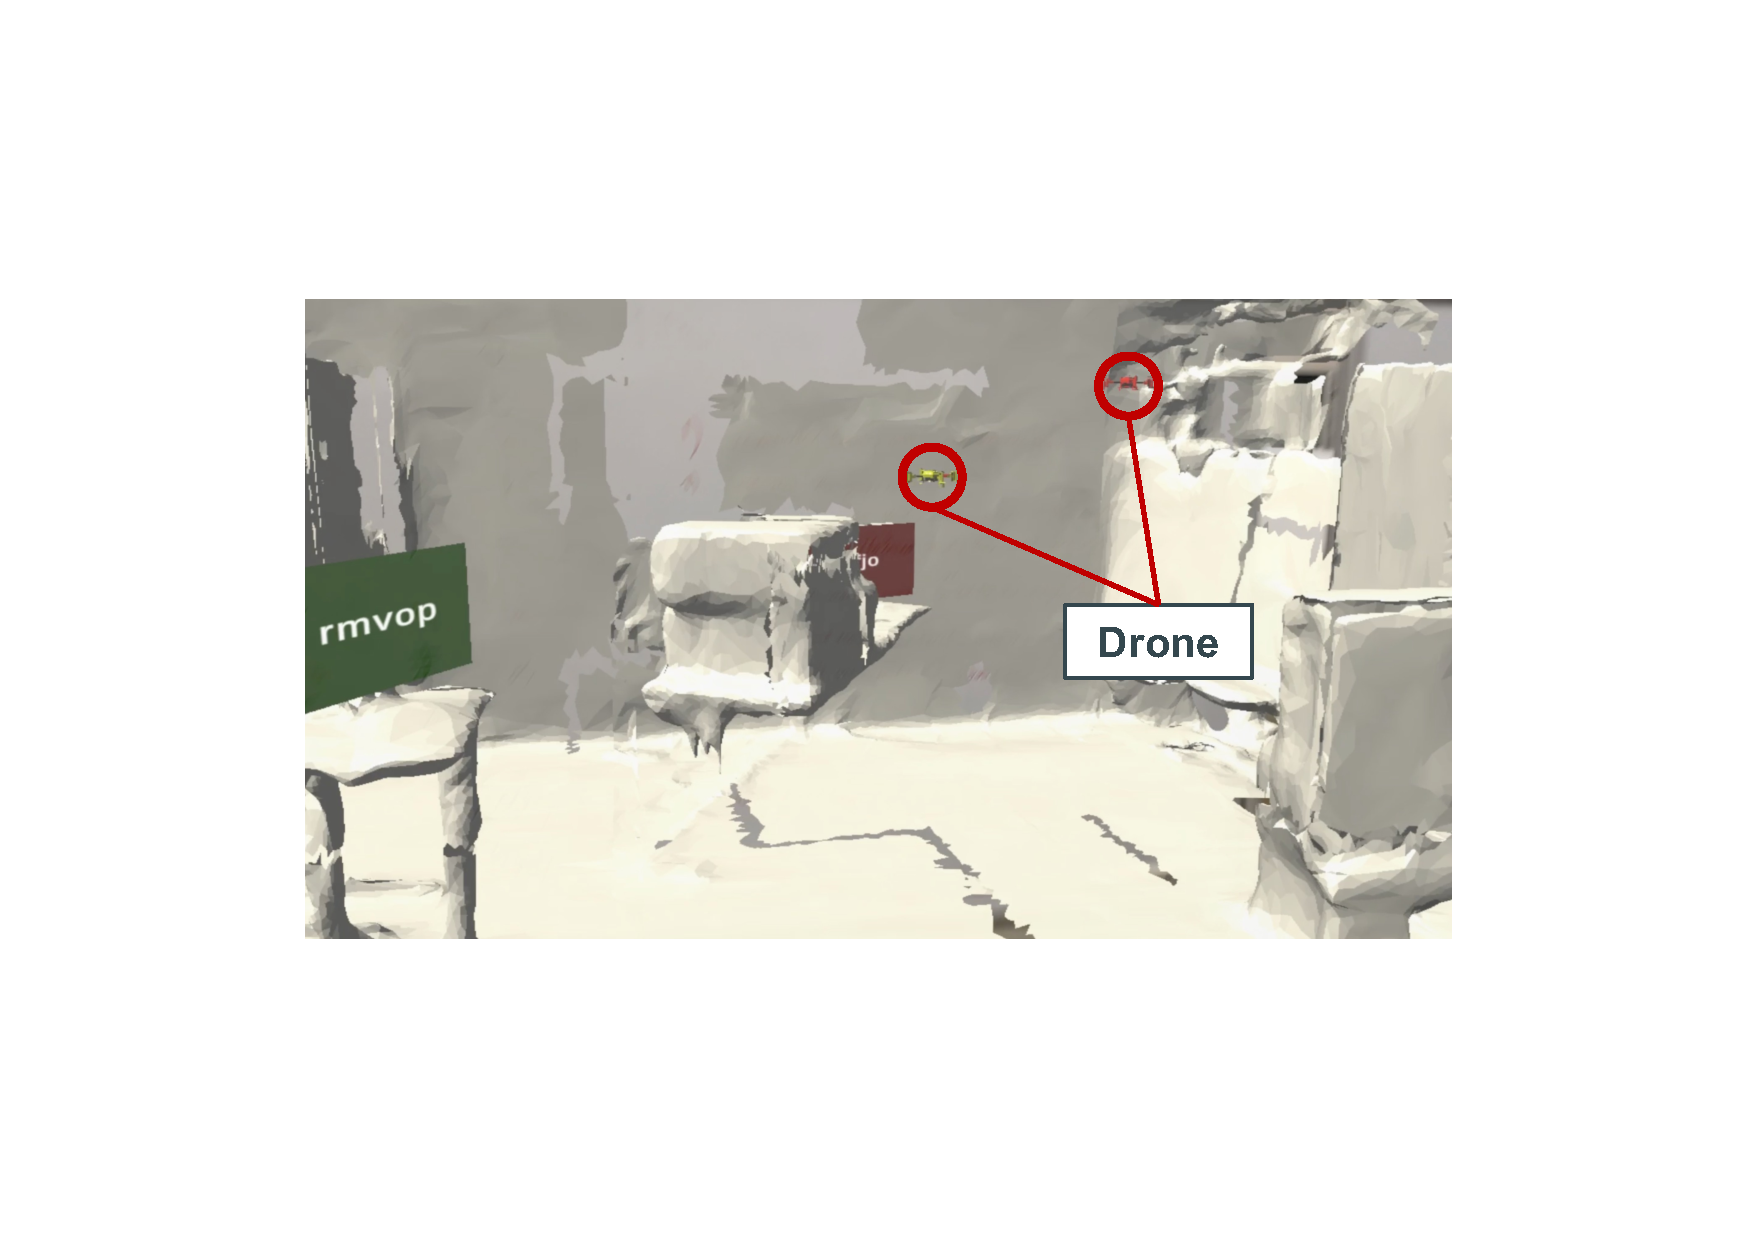
\includegraphics[width=\linewidth]{img/03_propose.pdf}
  \caption{提案方式の操縦者目線}
  \label{fig:03_propose}
\end{figure}


\section{遮蔽物との距離を考慮した危険度の付与}
\label{sec:DangerLevel}

\ref{sec:ARvisualize}節で述べたように,ARを利用することで操縦者とドローン間に位置する遮蔽物を透過することで,死角領域内を可視化している.
しかし,遮蔽物を完全に透過することによって,遮蔽物を全く意識しないドローン操縦を行うことになり,遮蔽物への衝突危険性を向上させてしまうことが推測できる.
\par
例えば,遮蔽物を完全に透過することにより,操縦者はドローンが死角領域内のどこを飛行しているのかは把握できている一方で,ドローンを操縦者がいる方向へ移動させたい場合,
透過されている遮蔽物がどのような形状をしているかも把握できないため,どこまでドローンを移動させることができるのか判断することができない.
そのため,遮蔽物を完全に透過するのではなく,ドローン周辺に位置する遮蔽物に対しては,動的に透明度を変更させる機能を実現させる必要性がある.

また,操縦者とドローンの間に遮蔽物が一つしかないとは限らない.
複数の遮蔽物が存在し,同じ透過度の遮蔽物が重なる場合,どの遮蔽物がドローンに最も近傍であるか認識できなくなり,操縦性の低減や遮蔽物・障害物への衝突危険性を向上させてしまうことが推測できる.
そのため,ドローンから距離の遠い遮蔽物の透明度を向上し,ドローンから距離の近い遮蔽物の透明度を低下することにより,ドローン周辺の遮蔽物を強調表示し,操縦者目線では認識が困難な遮蔽物の形状を把握できる機能を開発する.
その上,\cite{tech-01}を参考に,ドローンから遮蔽物までの距離に応じて,障害物の色を分けている.
障害物を3色に分類することで,近傍の障害物の危険性を警告する.
\par
提案方式では,障害物までの危険な距離を0.3m ,未だ猶予はあるが慎重に動くべき距離を0.6m とする.
常に操縦者とドローン間に位置する遮蔽物までの距離を計測し,閾値を元に以下のいずれかの動作をする.

\begin{enumerate}
	\item ドローンからの距離が0.3m 未満の遮蔽物を赤色に変更
    
  \item ドローンからの距離が0.3m 以上 〜 0.6m 未満の遮蔽物を赤色から黄色に変更
    
  \item ドローンからの距離が0.6m 以上 〜 1.0m 未満の遮蔽物を赤色から緑色色に変更
  
  \item ドローンからの距離が1.0m 以上の遮蔽物を完全に透過
\end{enumerate}

\figref{fig:03_dangerLevel1},\figref{fig:03_dangerLevel2}に示すように,遮蔽物の重なりの可視化による情報過多を防いだ上で,ドローン周辺の障害物の危険度を理解できる,色彩の変化による視覚支援を行なっている.
赤色に変化した障害物の方向には衝突の危険性,黄色になっている障害物の方向には慎重な操縦の必要性,一方で緑色の障害物の方向には進んでも衝突の危険性がないことを示し,操縦者への安心感を提供する遮蔽物知覚を行っている.

% 上の図と比較してわかるように表現
\begin{figure}[!tb]
  \centering
  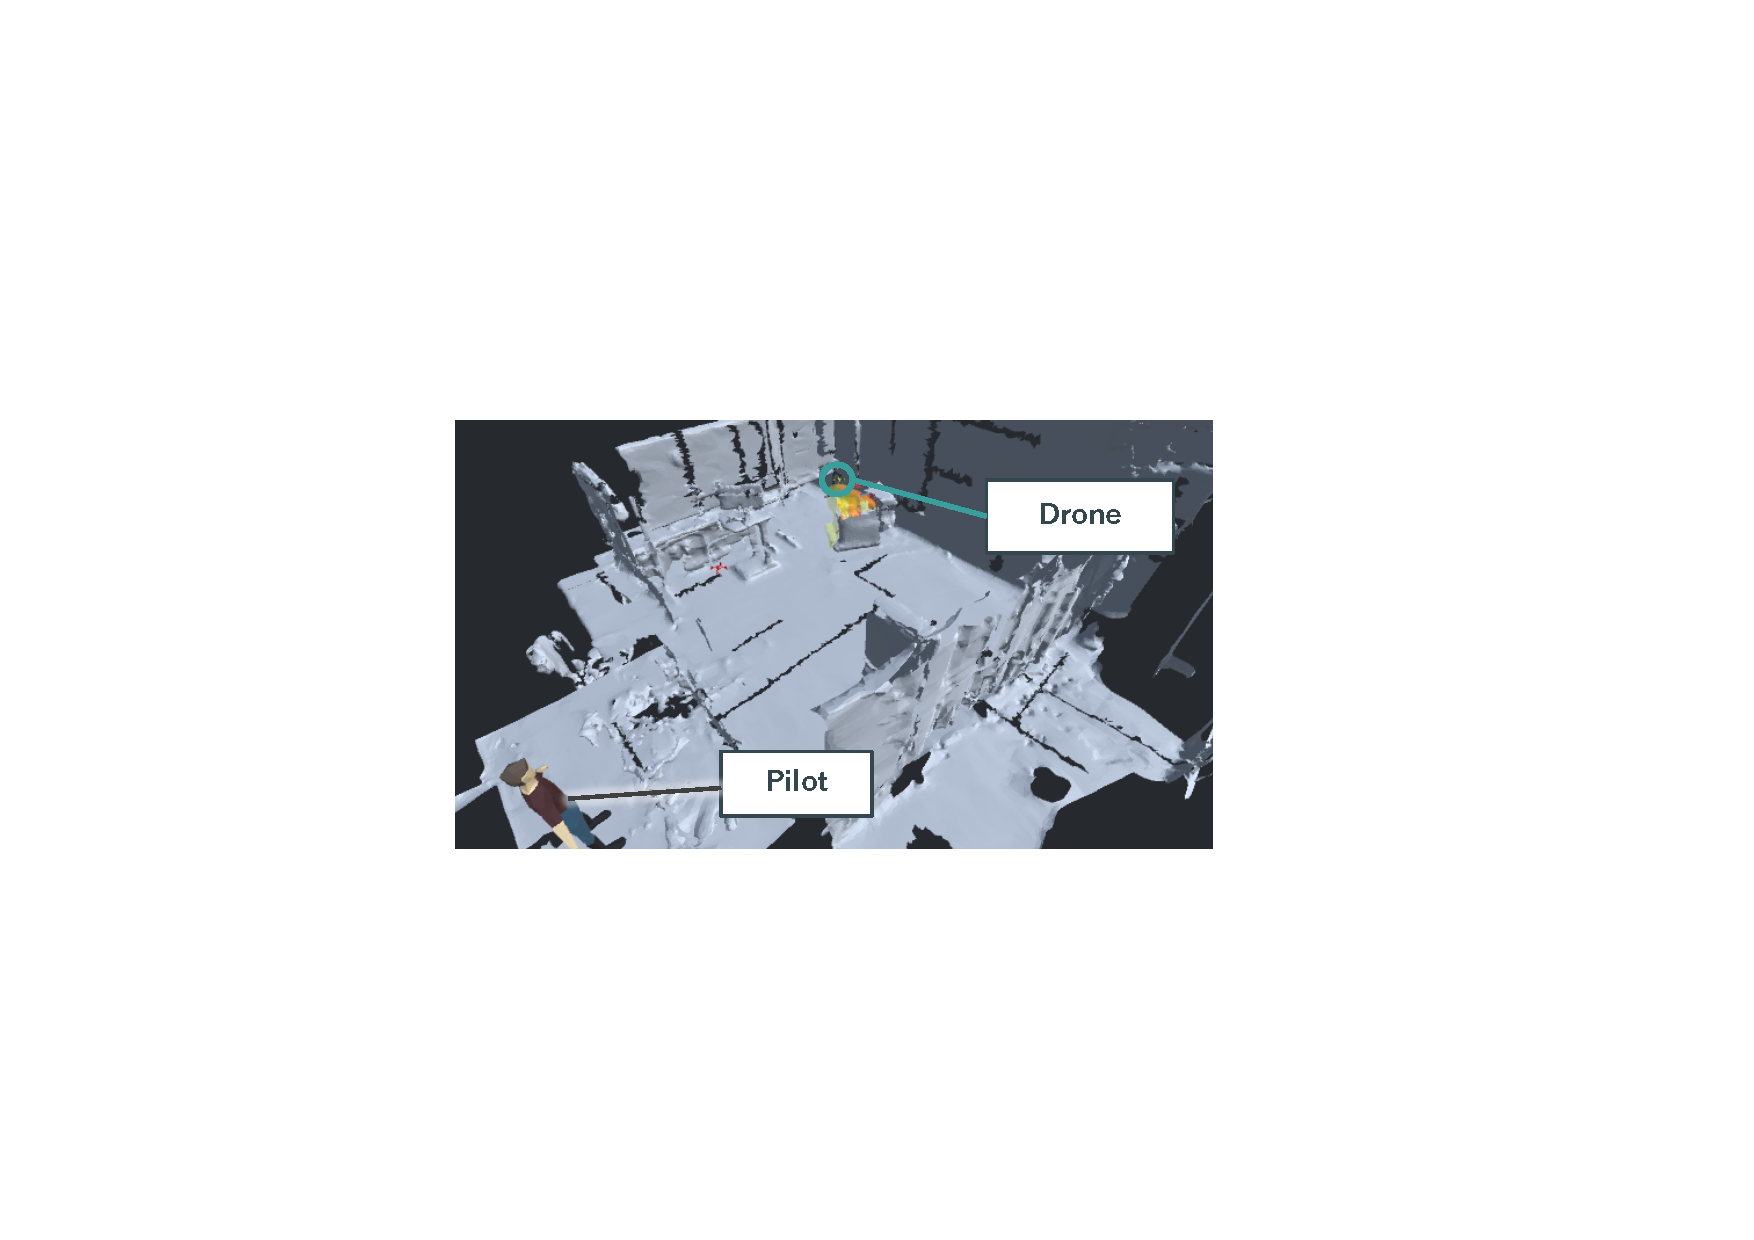
\includegraphics[width=0.9\linewidth]{img/03_danger1.pdf}
  \caption{操縦者目線での遮蔽物知覚}
  \label{fig:03_dangerLevel1}
\end{figure}
\begin{figure}[!tb]
  \centering
  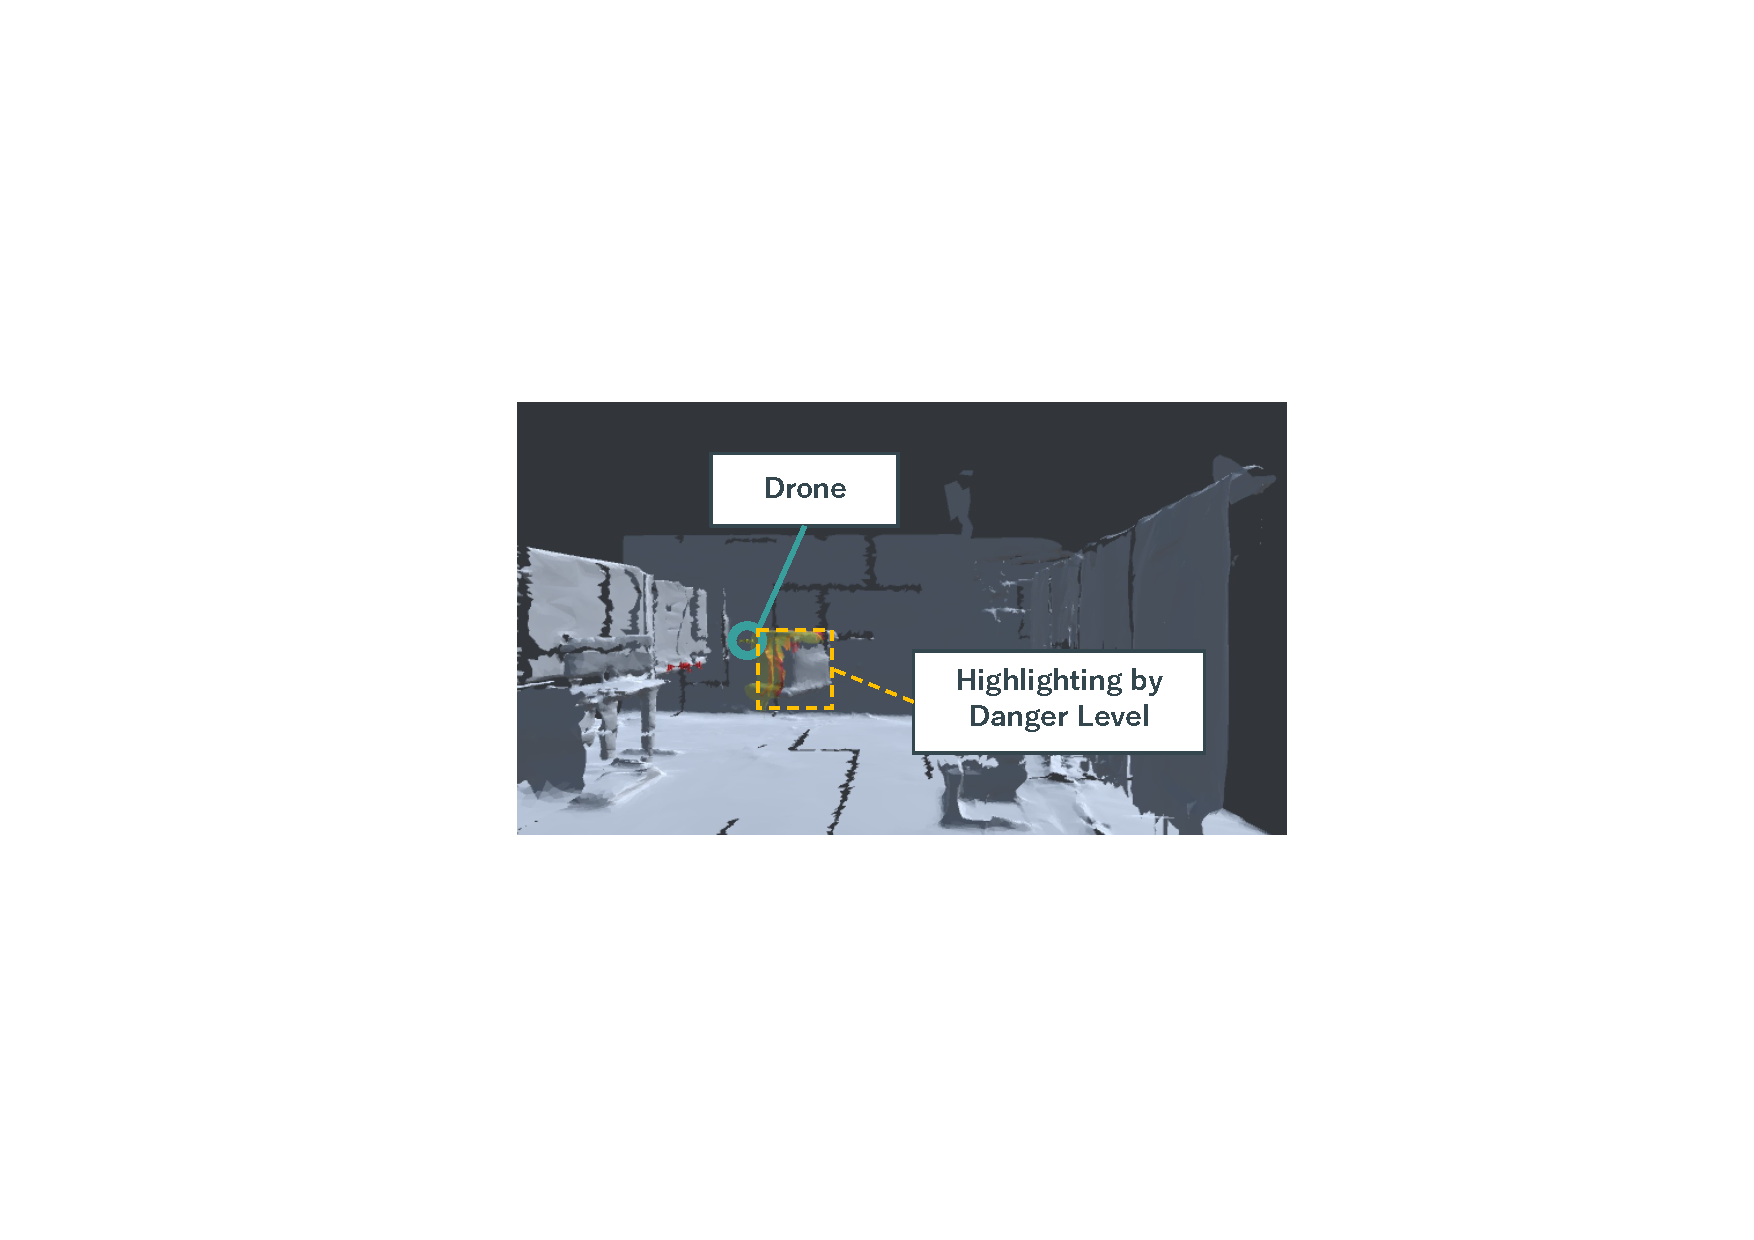
\includegraphics[width=0.9\linewidth]{img/03_danger2.pdf}
  \caption{三人称視点での遮蔽物知覚}
  \label{fig:03_dangerLevel2}
\end{figure}

%----------------------------------------------------------------------
% 実装
%----------------------------------------------------------------------
\chapter{実装}
\label{chap:Development}

% ******************** Section ********************

\section{実装環境}
\label{sec:DevEnviroment}

ハードウェアとソフトウェアのコンポーネントとそれらの間のデータフローを含む,
実験システムアーキテクチャの詳細な概要を\figref{fig:04_system}に示す.

各ドローンを制御するコンピュータでは Ubuntu18.04を使用しており,ドローンと通信を行なっている.
ドローンはRyze Tech社製Tello EDU(以下,Tello)\cite{web-tello}を使用しており,vSLAMであるORB-SLAM2\cite{article-slam}を利用し,自己位置推定,画像処理による点群データの抽出を行なっている.
取得した点群はPCL(Point Cloud Library)\cite{book-pcl}による処理を通した上で,サーバに送信している.
サーバではTello,ARHMDとSocket通信を行なっており,常時,Telloの傾きや移動距離をARHMDに送信する.
ARHMDはMicrosoft HoloLens2(以下,HoloLens)\cite{web-hololens}を使用する.
HoloLensはWi-Fi経由で通信を行い,受け取ったデータをゲーム・アニメーションエンジンであるUnity \cite{web-unity}座標系へ変換し,変換後の値を反映させることにより,操縦者へ視覚支援を行う.
事前に,HoloLensのSpatial mapping\cite{web-spatial}により空間マッピングを行うことで空間のメッシュデータを入手し,静的な三次元環境地図を作成する.
作成した三次元環境地図を,Unity内の3D仮想空間上に配置し,操縦者の位置情報と,Unity内の三次元環境地図の位置合わせを行うことで,空間認識を提供する.
また,実験を行う中で,実験協力者よりARによる可視化の遅延を提示されたことはなく,実験で戸惑うこともなかったため,ARによる可視化の遅延が操縦に影響を与えることはない.

全てのコンポーネントはEthernet,Wi-Fiを介して通信を行い,ソフトウェアコンポーネントは,ROSノード\cite{ros}を介したPublish/Subscribe通信を行なっている.
実装で使用したハードウェアの一覧を\tabref{tab:hardware_structure}に示す.

また,複数ドローンが飛行する中,自身の操縦する仮想ドローンを特定できるよう,各仮想ドローンの色を変更している.
その上,仮想ドローンが向いている方向がわかるように,前方には目印をつけている.

\begin{figure}[!tb]
  \centering
  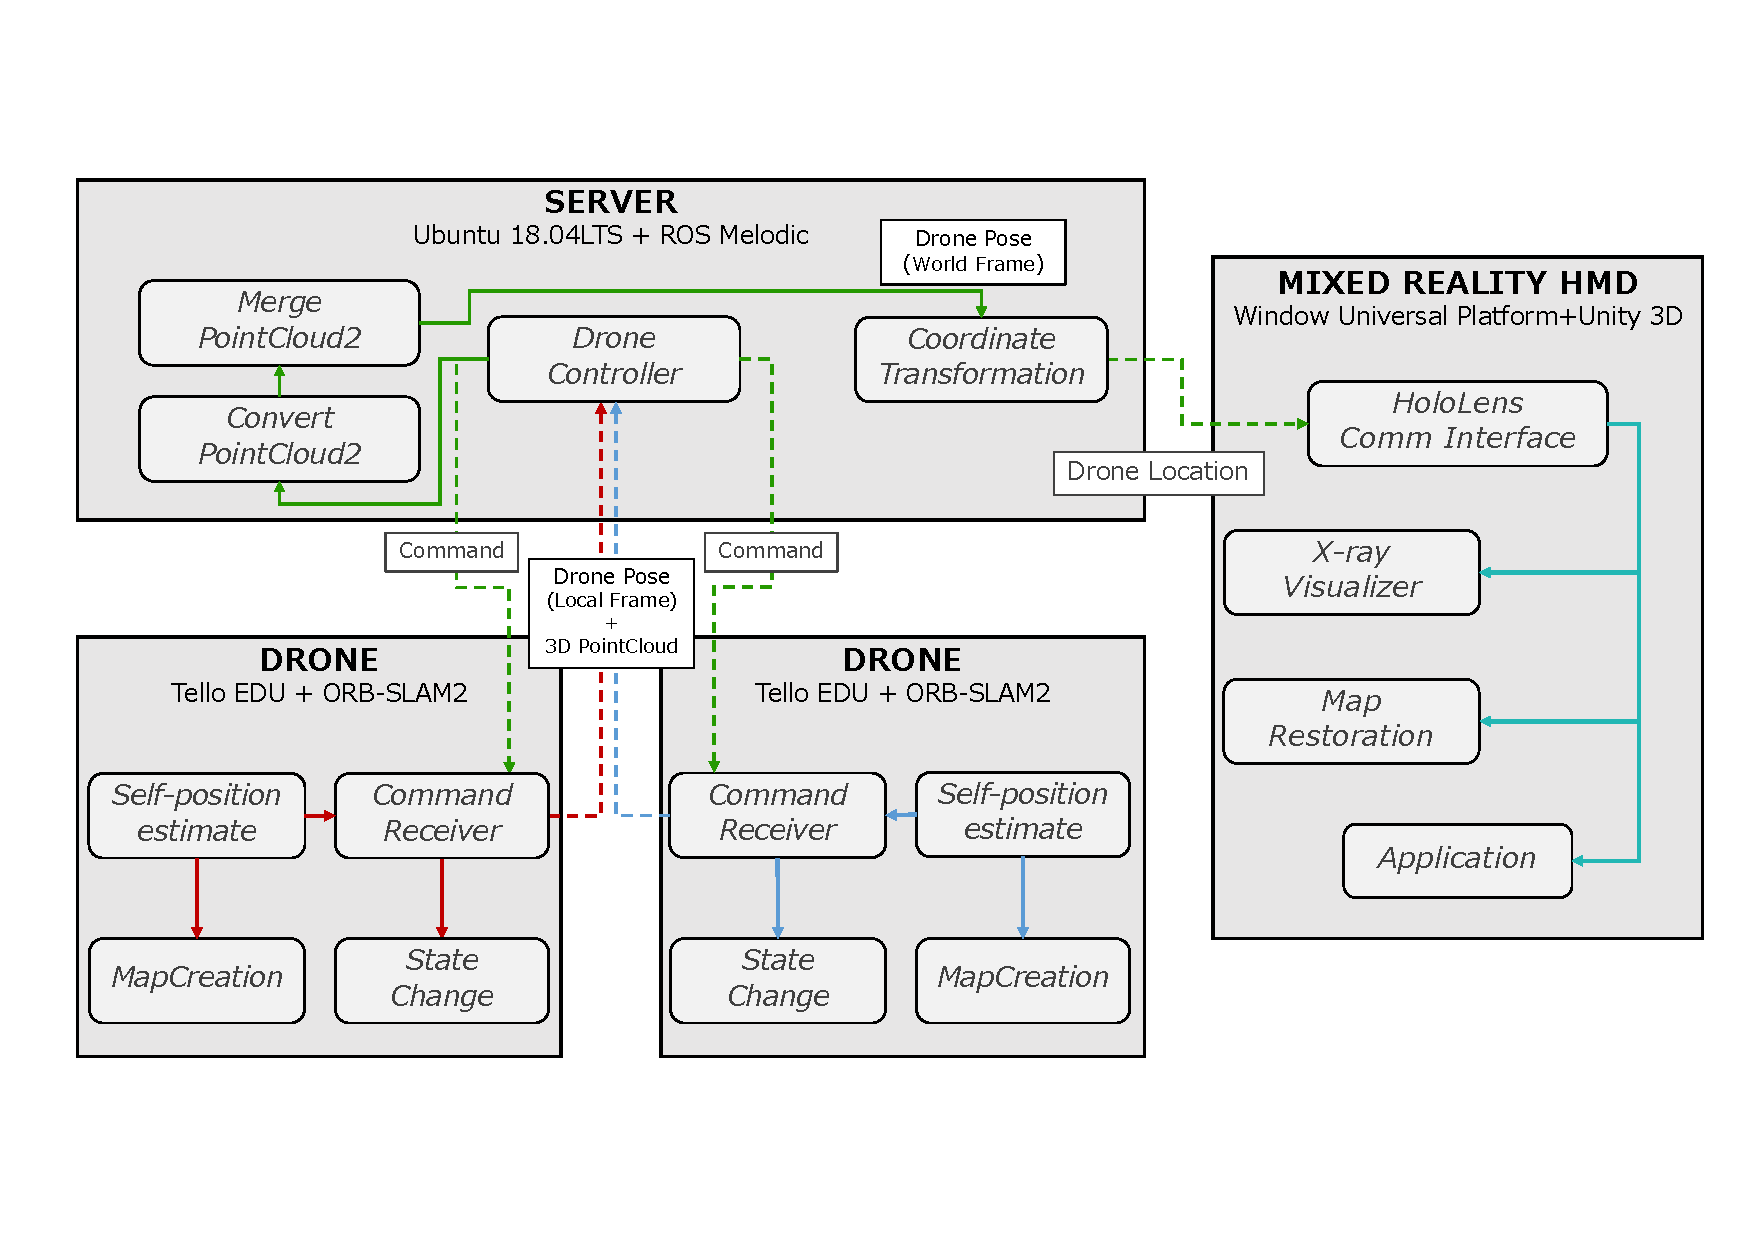
\includegraphics[width=\linewidth]{img/04_system.pdf}
  \caption{システム構成}
  \label{fig:04_system}
\end{figure}

\begin{table}[!t]
  \caption{提案方式のハードウェア構成}
  \label{tab:hardware_structure}
  \centering
  \begin{tabular}{ccc}
    \hline\noalign{\smallskip}                                      \\
    \noalign{\smallskip}\hline\noalign{\smallskip}
    \multirow{4}{*}{サーバ} & CPU    & Intel Core i9-12900H (6P-Core + 8E-Core 20thread) \\
                                            & GPU    & Intel Iris Xe Graphics / RTX 3050 Ti               \\
                                            & OS    & Ubuntu18.04 (ROS Melodic)                                 \\
                                            & メモリ & 16 GB (LPDDR5-5200)                           \\
                                            & SSD    & 1TB(M.2 NVMe PCIe 4.0 x4)                                 \\
    \noalign{\smallskip}\hline\noalign{\smallskip}
    \multirow{2}{*}{ドローン}              & メーカ & Ryze Tech                                        \\
                                            & 品名   & Tello EDU                            \\
    \noalign{\smallskip}\hline\noalign{\smallskip}
    \multirow{2}{*}{ARHMD}              & メーカ & Microsoft                                       \\
                                            & 品名   & HoloLens2                               \\
    \noalign{\smallskip}\hline
  \end{tabular}
\end{table}


% \begin{table}[tb]
%   \caption{車両が送信するUDPパケット}
%   \label{tab:vehicle_udp_packet}
%   \centering
%   \begin{tabular}{ll}
%     \hline\noalign{\smallskip}
%     Data category & Size       \\
%     \noalign{\smallskip}\hline\noalign{\smallskip}
%     IP header     & 40 Byte    \\
%     UDP header    & 8 Byte     \\
%     Custom header & 80 Byte    \\
%     Payload       & 1,030 Byte \\
%     \noalign{\smallskip}\hline
%   \end{tabular}
% \end{table}

\section{ドローンの飛行制御}
\label{sec:ControlDrone}

実際に使用したドローンは\figref{fig:04_drone}に示す.
また,操縦するためのコントローラではキーボードを用いている.

Telloはプログラミングによってフライトコントロールを行うことができ,規定のコマンドを送信することで飛行制御することができる.
キーボードとTelloのコマンドを結びつけ,キーボードを押下することによりコマンドを実行し,ドローン操縦を行なっている.
キーボードを押下する強さや長さによってドローンの速度を増減させることができ,操縦者の意思を反映できるよう開発している.

また本研究では,vSLAMを用いた自己位置推定を行なっており,キーボードを押下することによって命令されたコマンドをもとに移動しながら,周辺環境を見渡すことで,
自身の位置情報を獲得している.
\figref{fig:04_feature}に示すように,ドローンのカメラ映像に対して画像処理を行うことで,カメラで撮影した1フレームの画像から,物体の端などのコーナー部分を特徴点として検出している.
その際,カメラで取得した画像から,周囲の環境の3次元構造を計算し点群データによる環境地図を作成している.
その地図に対し,自身がどのくらい動いたかによって位置を推定する.

この際,ドローンに搭載されたカメラのキャリブレーションを事前に行なっている.
カメラキャリブレーションとは,レンズ焦点距離などの内部パラメータと,カメラの位置・姿勢を表す外部パラメータ,レンズの歪収差係数を求め,画像を補正する処理のことである.
カメラパラメータを得るための方法として,OpenCV\cite{article-opencv}でも実装されている,平面マーカを用いたZhangの手法\cite{article-zhang}を利用した.
\figref{fig:04_calibration}に示すようなチェスボードを利用し,ドローンごとにキャリブレーションを行った.



% 図で表現
\begin{figure}[!tb]
  \centering
  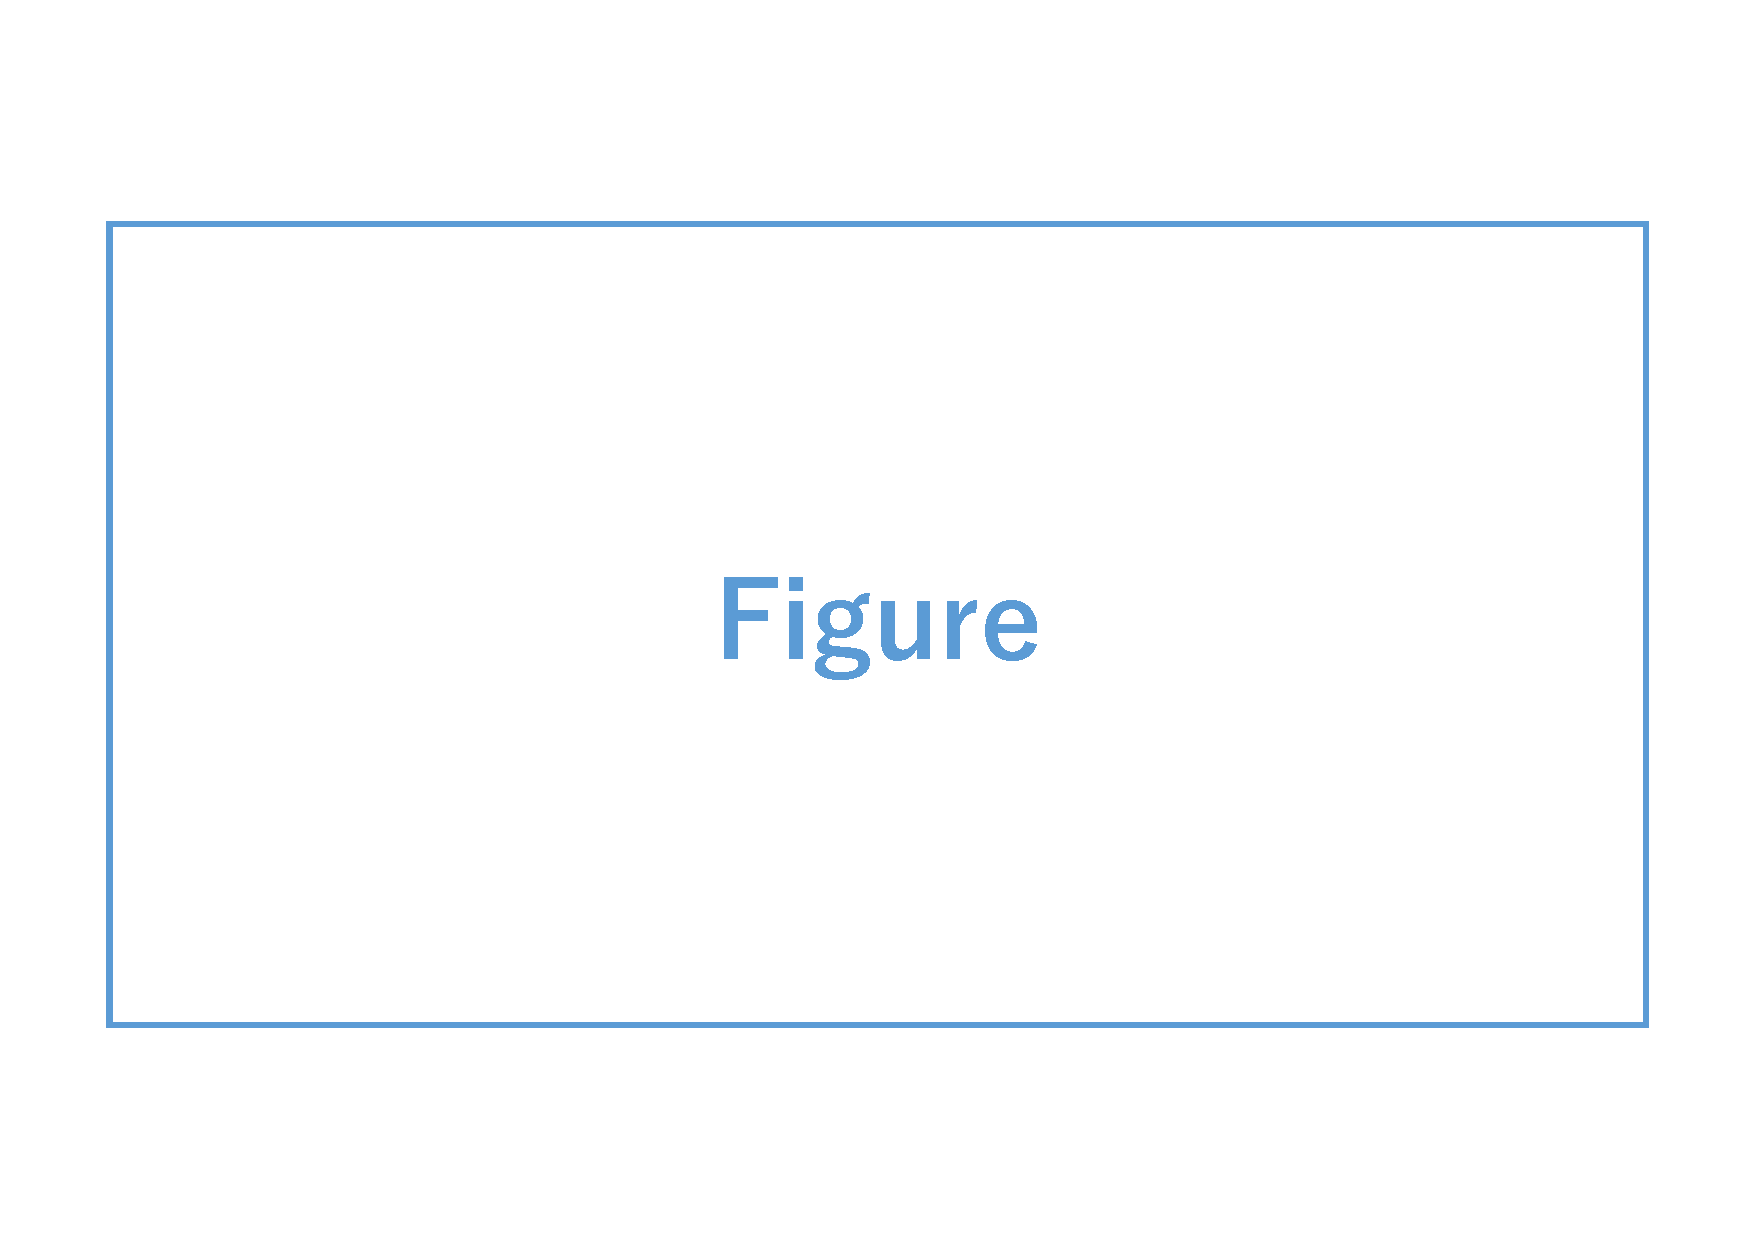
\includegraphics[width=0.7\linewidth]{img/sample.pdf}
  \caption{実験で使用したドローン}
  \label{fig:04_drone}
\end{figure}

\begin{figure}[!tb]
  \centering
  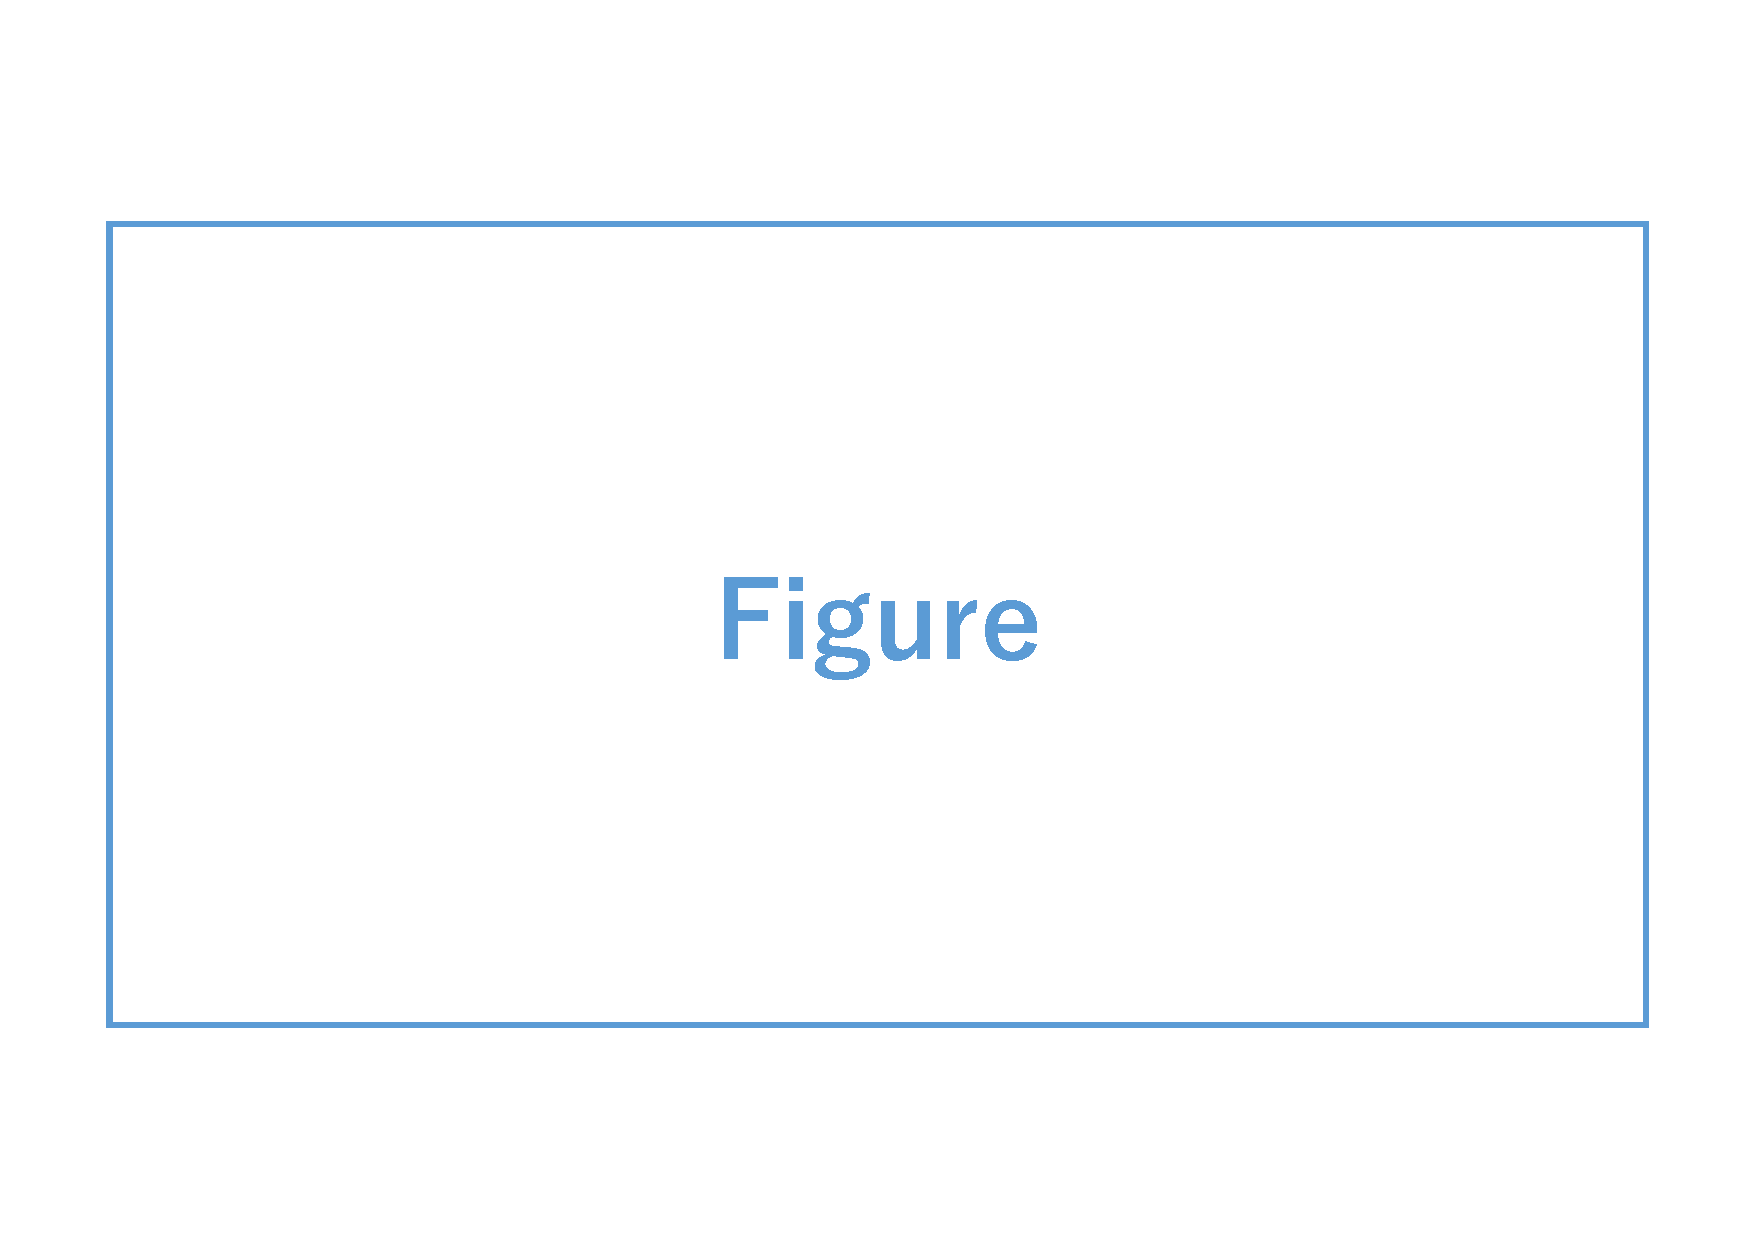
\includegraphics[width=0.7\linewidth]{img/sample.pdf}
  \caption{特徴点抽出}
  \label{fig:04_feature}
\end{figure}

% 図で表現
\begin{figure}[!tb]
  \centering
  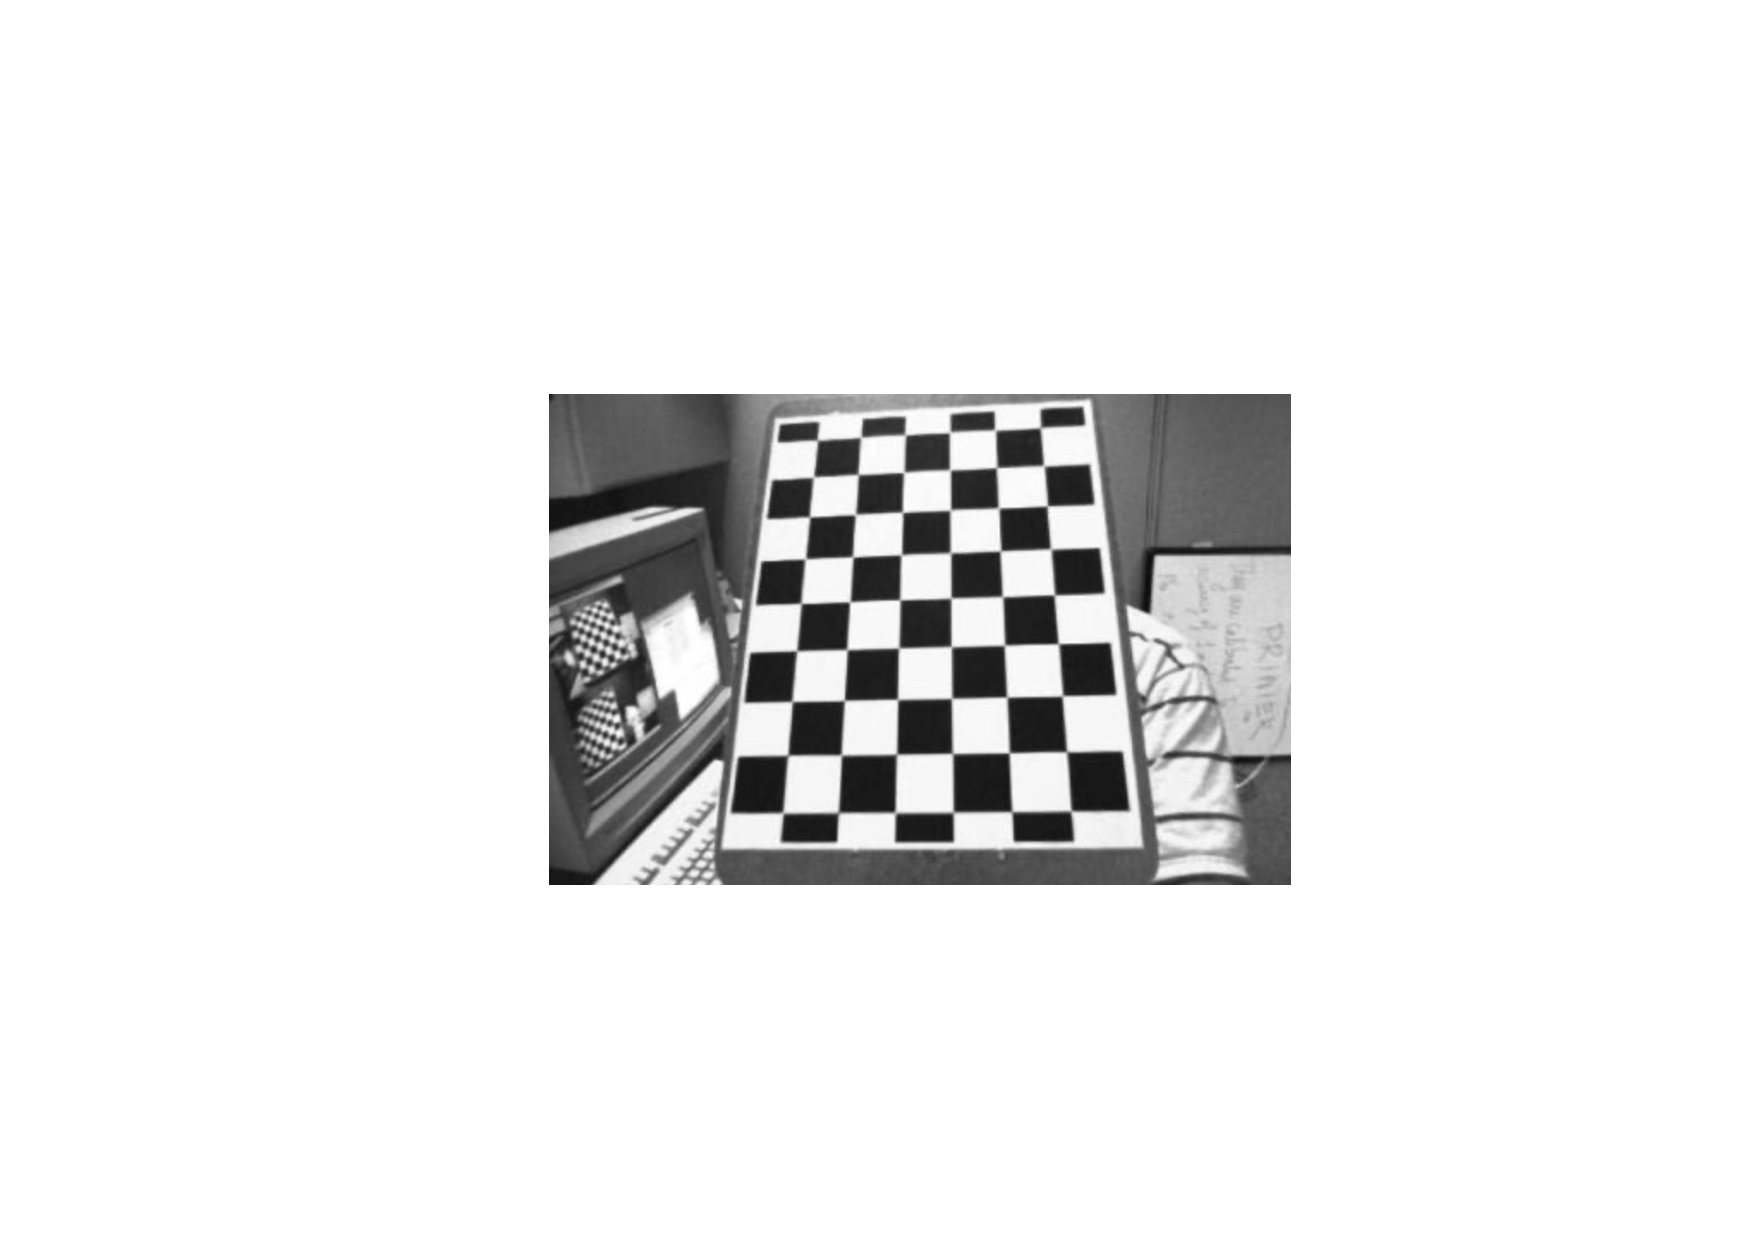
\includegraphics[width=0.7\linewidth]{img/04_calibration.pdf}
  \caption{キャリブレーションで使用したチェスボード}
  \label{fig:04_calibration}
\end{figure}


\section{障害物への衝突警告}
\label{sec:CollisionWarning}

本研究では,実験途中のクラッシュによる実験中止を避けるため,衝突する直前に操縦者に対して警告音を出している.
具体的には,AR表示されている三次元環境地図と仮想ドローンの距離が0.3m 以内に達した場合に,操縦者へ衝突警告音を出し,操縦者のドローン操縦を強制的に止めている.
これは,ドローンが決められた幅の枠を通過する際に,枠の幅が0.3m の場合にドローンと枠が衝突する危険性が向上していたため\cite{tech-01},
本研究の実験環境の中でドローンを一定の枠の幅で動作させる際も,ドローンの位置と枠の距離が0.3m 以内の場合には衝突危険性が増加すると判断し,衝突の危険性の距離を0.3m としている.
仮想ドローンと三次元環境地図との距離が0.3m より大きくなった際に,警告音を止めている.

\figref{fig:04_warning}に示すように,仮想ドローンの周辺には衝突検知網を張っており,三次元環境地図との距離が0.3m に達した場合に警告音を出し,操縦を一時的に止める.
以降は,ドローンを移動させた際の仮想ドローンと三次元環境地図との距離が,衝突警告音を出した際の仮想ドローンと三次元環境地図との距離より短くなっていれば再度操縦を強制的に止め,
距離が長くなっていれば,操縦を許可する.

% 図で表現
\begin{figure}[!tb]
  \centering
  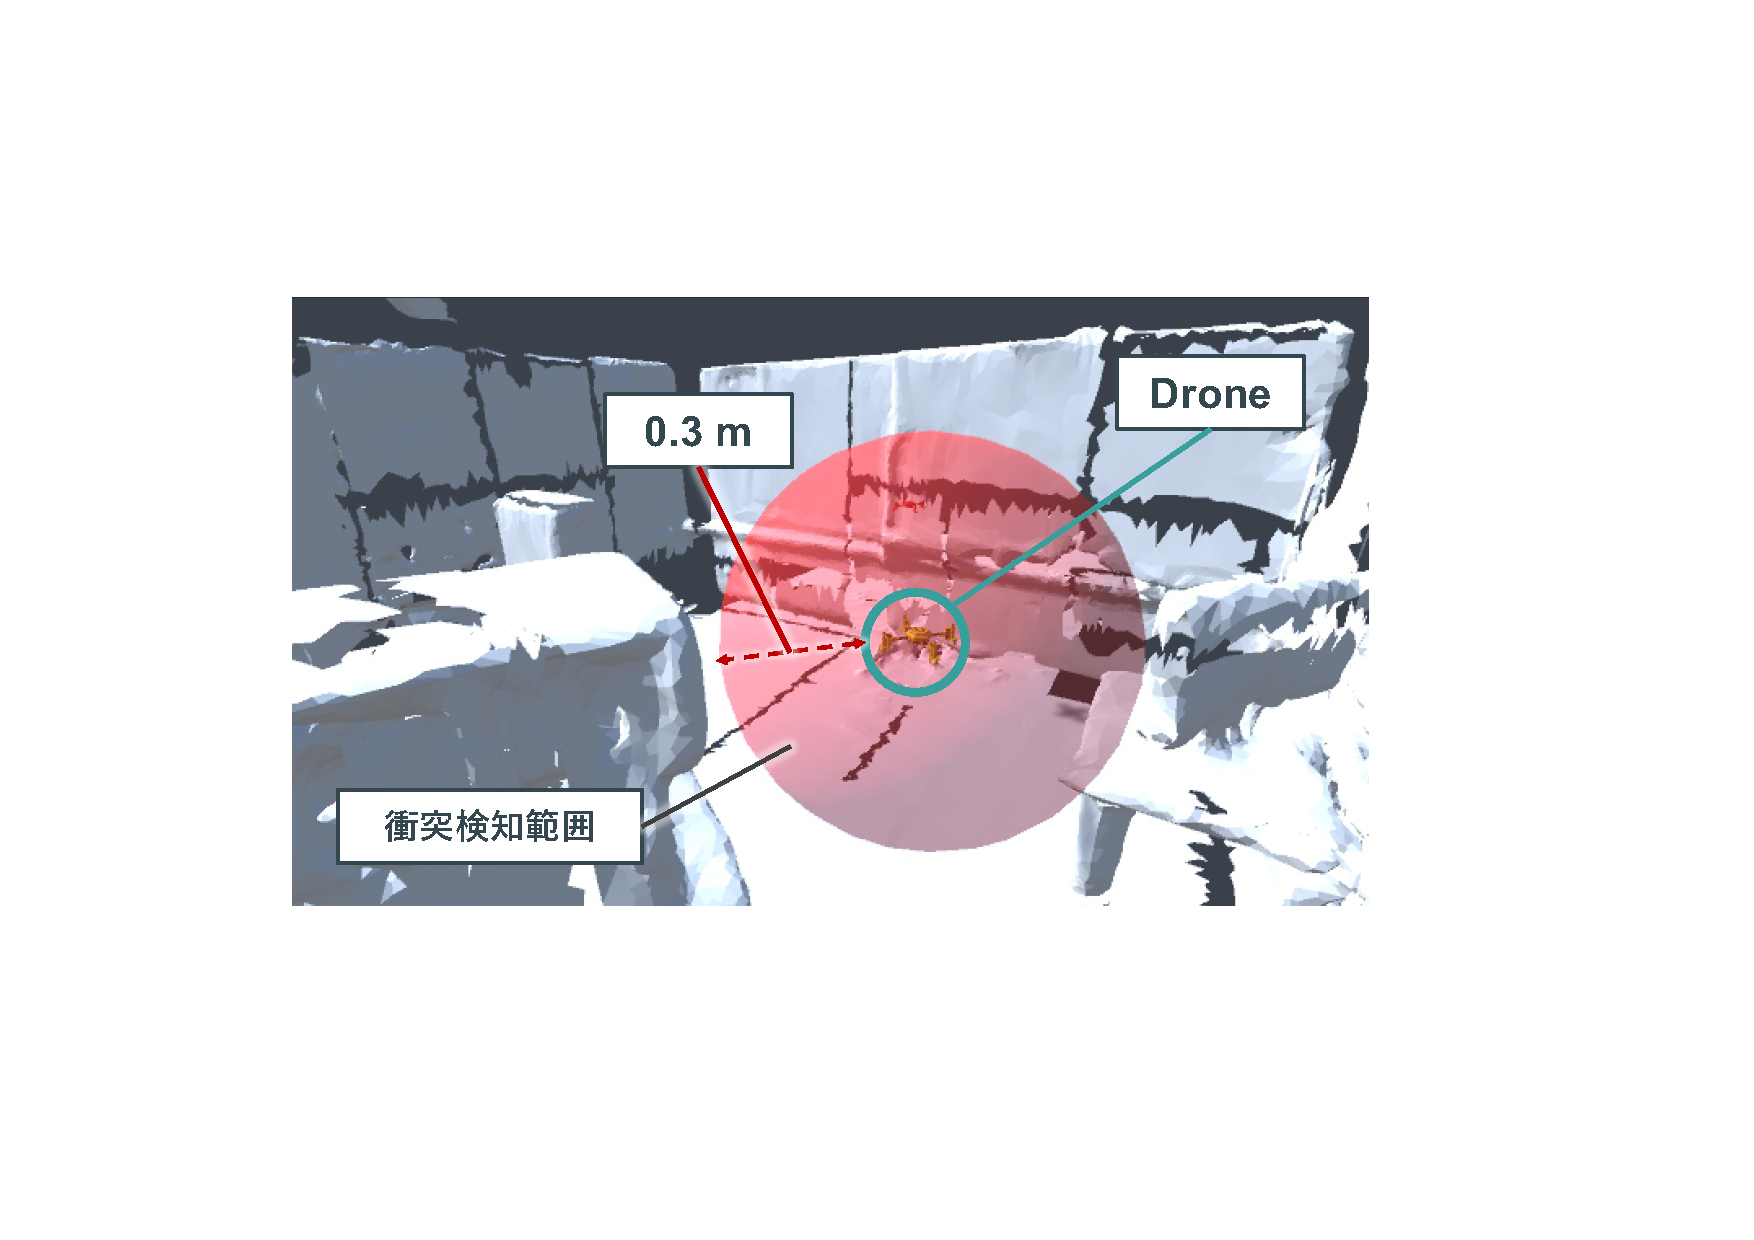
\includegraphics[width=0.7\linewidth]{img/04_warning.pdf}
  \caption{周辺障害物との衝突検知}
  \label{fig:04_warning}
\end{figure}

% \section{三次元環境の位置合わせ}

% tf変換を行い,その位置をUnity座標へ変換
% 事前に静的な環境を取得
% 位置合わせを行い,三次元環境地図をBlenderにて細分化
% 2台のドローンを操作するコンピュータとWi-Fiを経由して通信
% 各ドローンが起動する位置,HoloLensが起動する位置が各機器のワールド座標となる
% そのため,スタート位置を事前に決めておき,設定したワールド座標からの差分をあらかじめ取得しておく
% 各ローカル座標を統一のワールド座標へ置き直し,位置合わせを行う
%----------------------------------------------------------------------
% 評価
%----------------------------------------------------------------------
\chapter{評価}
\label{chap:Experiment}

% ******************** Section ********************
\section{比較方式}
\label{sec:ComparisonMethod}
% 従来方式、可視化方式の説明
先に述べた関連研究\cite{article-ar05}を元に,本研究では2つのドローン操縦方式を用意し,二人称視点方式,可視化方式と呼ぶものとする.
\figref{fig:05_fpv}に示す,ドローンが撮影する映像を頼りに操縦を行う従来のドローン操縦手法である二人称視点方式と,\figref{fig:05_visualization}を参考に作成した,ARを用いて死角領域内の空間認識を提供することにより,一人称視点でのドローン操縦を可能とした可視化方式を提案方式と比較することにより,どのような情報が未知領域探査効率を向上させ,ドローン操縦の安全性向上を示せるか評価する.
\par
可視化方式では,ドローンと操縦者の間に遮蔽物が存在する場合,ドローンが飛行している場所が操縦者にとっての死角領域となる.
死角領域が存在すると判断したとき,事前に空間マッピングした三次元環境地図における遮蔽物を透過した上で,現実環境に重畳表示することで,仮想的に死角領域の空間認識を提供する.
操縦者は,死角領域内を飛行するドローンを視認することはできないが,ARによって仮想のドローンと,ドローン周辺の三次元環境を視認することができる.
\figref{fig:05_visualization}に示すように,遮蔽物によって視認できないドローンと,そのドローン周辺の環境をARによって可視化している.
また,ドローン上部にドローンカメラ映像を映し出しており,常に操縦者の方向を向くことで,操縦者がどこにいてもカメラ映像を把握できるよう開発している.

% ******************** Section ********************
\section{タスク}
\label{sec:Task}

実験環境を\figref{fig:05_experiment}に示す.
ドローンを上下左右に移動しなければ衝突の恐れがあるよう障害物を設置し,赤色と緑色の異なる背景色で表示されたモニター2台を設置している.
モニター内にはランダムなテキストを表示しており,モニター内の文字は任意の距離から一意に識別できるよう設置している.
\par
また,実験環境には自身が操縦するドローンとは別に,もう一台ドローンが自律飛行しており,障害物だけでなく,もう一台のドローンにも衝突しないよう気をつける必要がある.
\par
実験参加者は,スタート地点よりドローンを移動させ,2台のモニターに表示されたランダムなテキストを,赤色のモニター,緑色のモニターの順で報告し,ドローンを着陸させるタスクを行なった.
\figref{fig:05_experiment}に赤色の点線で示されている障害物を回避する必要があり,避けなければ通過が困難になるよう設定している.
実際の狭小空間では,速さだけではなく,衝突のない安全飛行が必要であるため,参加者にはタスクの早期終了ではなく,障害物にぶつかることなく,慎重に通過することを要求した.

\begin{figure}[!tb]
  \centering
  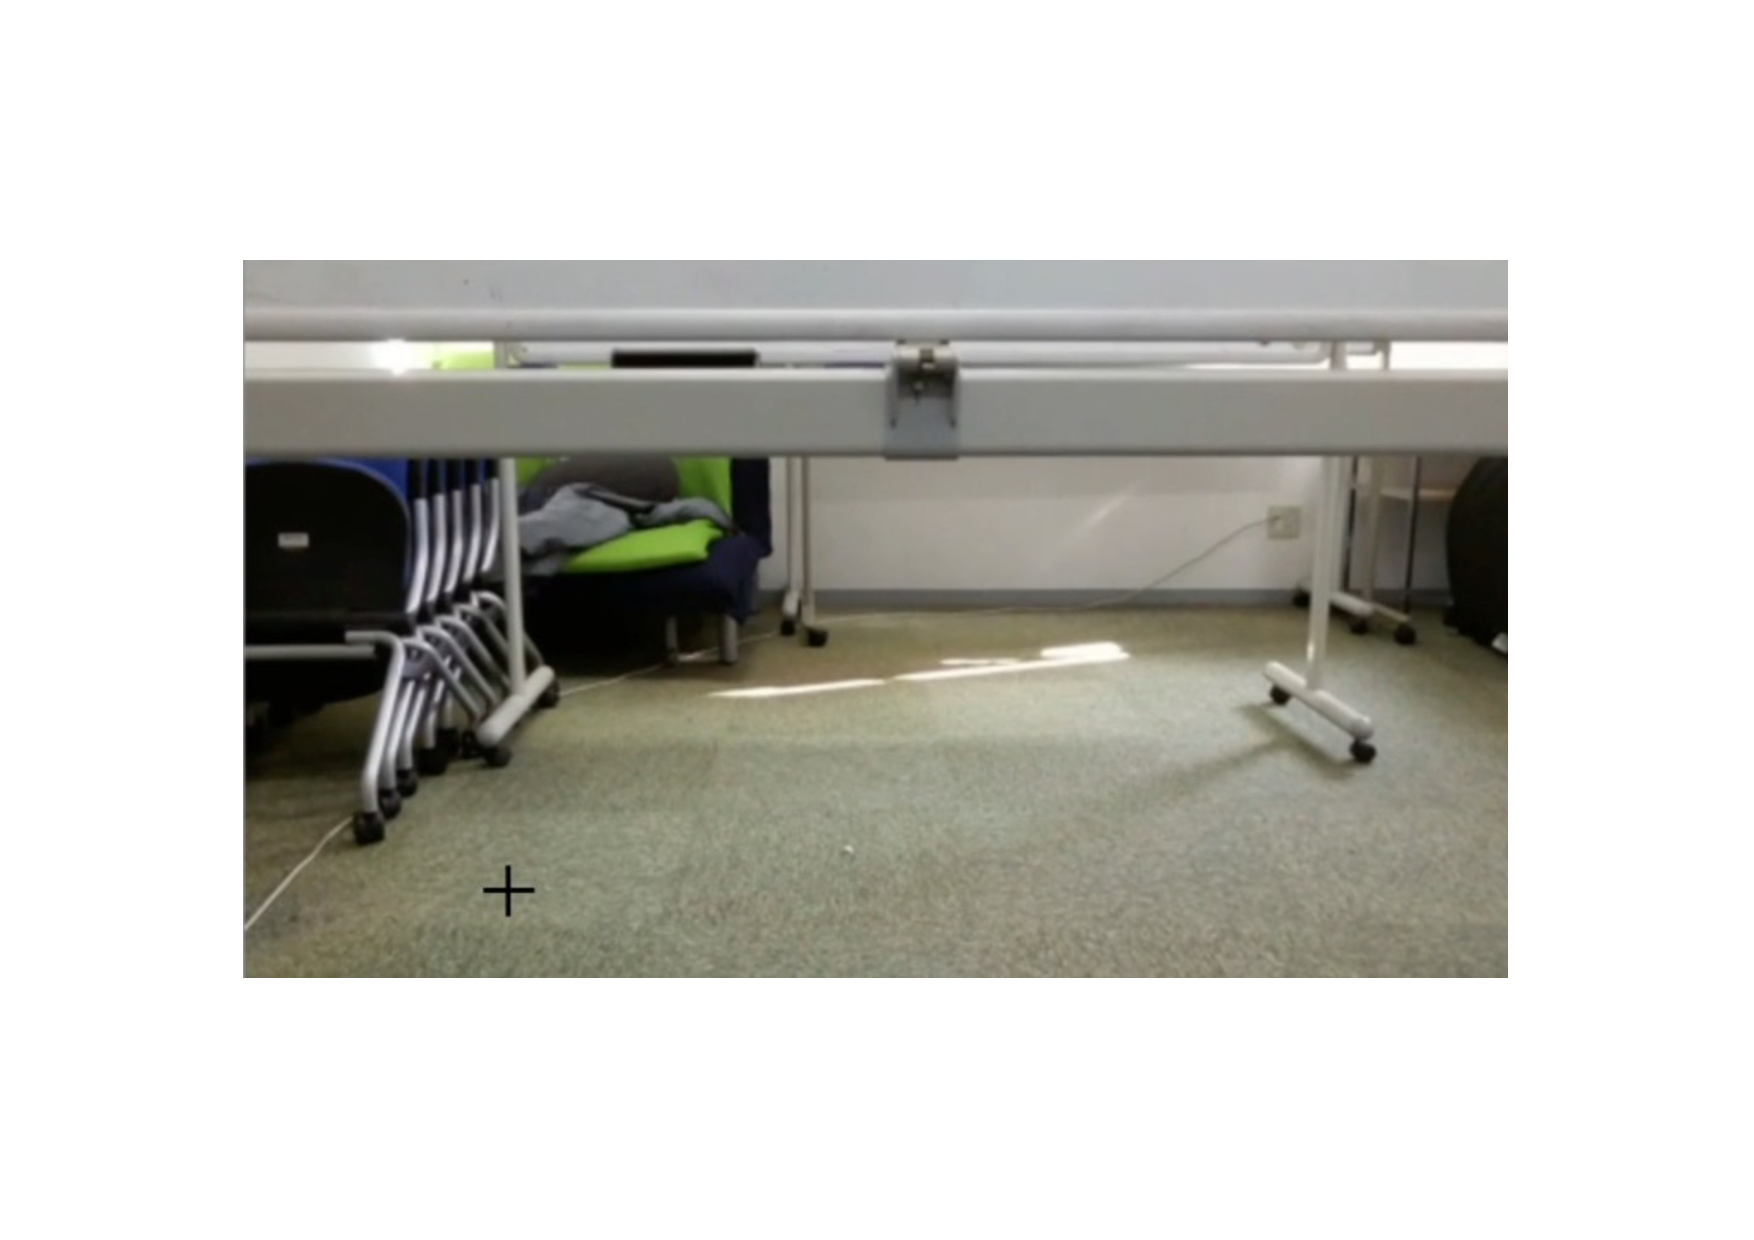
\includegraphics[width=0.7\linewidth]{img/05_fpv.pdf}
  \caption{二人称視点方式の操縦者目線}
  \label{fig:05_fpv}
\end{figure}

\begin{figure}[!tb]
  \centering
  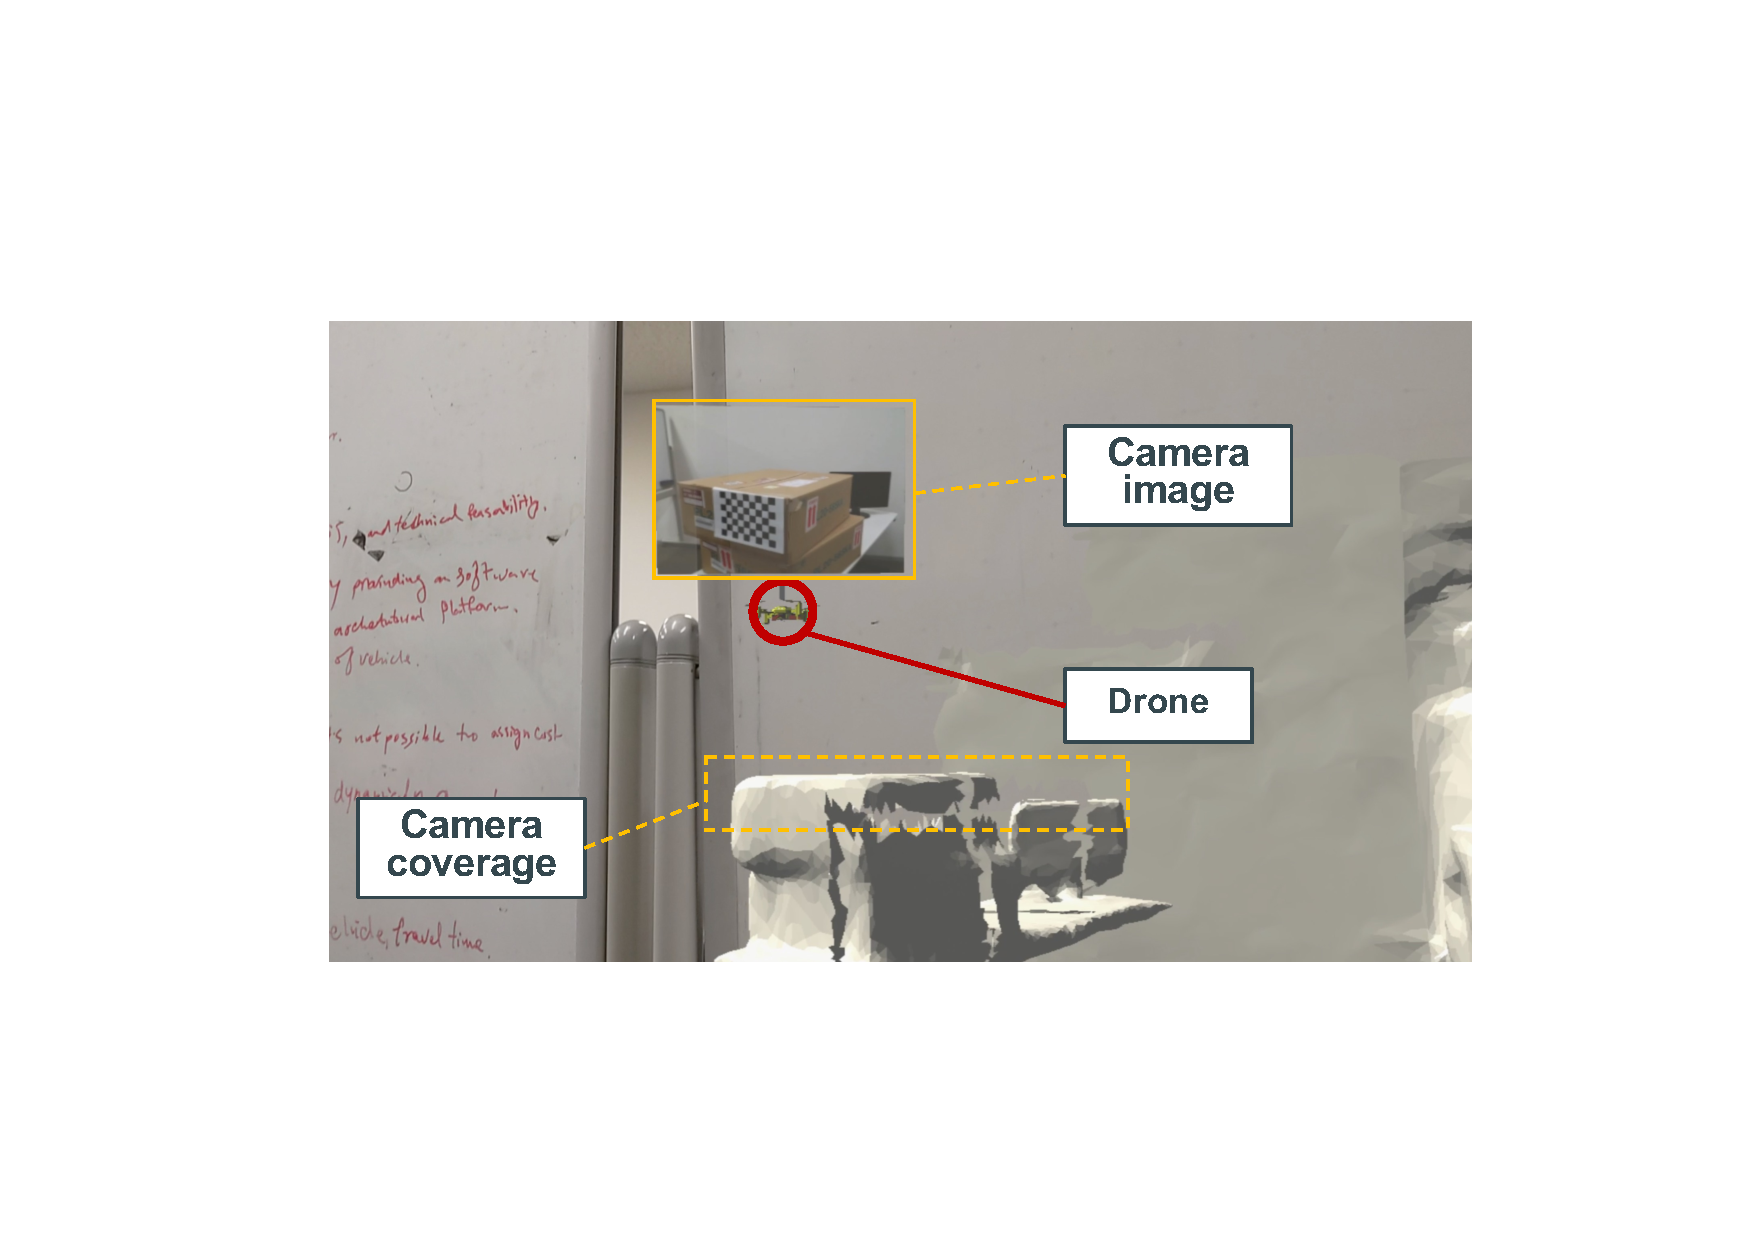
\includegraphics[width=0.7\linewidth]{img/05_visualization.pdf}
  \caption{可視化方式の操縦者目線}
  \label{fig:05_visualization}
\end{figure}

% ******************** Section ********************

\section{パラメータと評価項目}
\label{sec:Parametor}

未知領域探査では,衝突することのできない点検や,迅速な対応が求められる災害現場など,ドローンを素早く,安全に操縦することが求められる.
そのため,各方式における,操縦者がタスクを完了するまでの操縦時間,障害物への衝突警告回数,ドローン操縦の不安度の3項目による客観的な評価と,参加者へのアンケート,自由回答による主観的な評価を記録した.

本研究では,実際にドローンが障害物に衝突しないように,障害物へ衝突する直前に衝突警告を表示しており,衝突警告の回数を衝突警告回数としている.

ドローン操縦の不安度では,タスク完了までにドローンに移動命令を行なったコマンド総入力回数,ドローンに移動命令を行なった際の各命令のコマンド時間間隔を評価している.
本実験では,移動命令の総入力回数が少ないほど,タスクを行う上での無駄な動作が少ないと判断する.
また,各移動命令の時間間隔が短過ぎれば,ドローンを移動させることによる障害物への衝突を恐れており,時間間隔が長過ぎれば,どこへドローンを移動させれば良いのか分からないことによる思考時間の増加を招いていると判断する.
これら2項目をもとに各方式を比較し,ドローン操縦における不安度として考察する.

\begin{figure}[!tb]
  \centering
  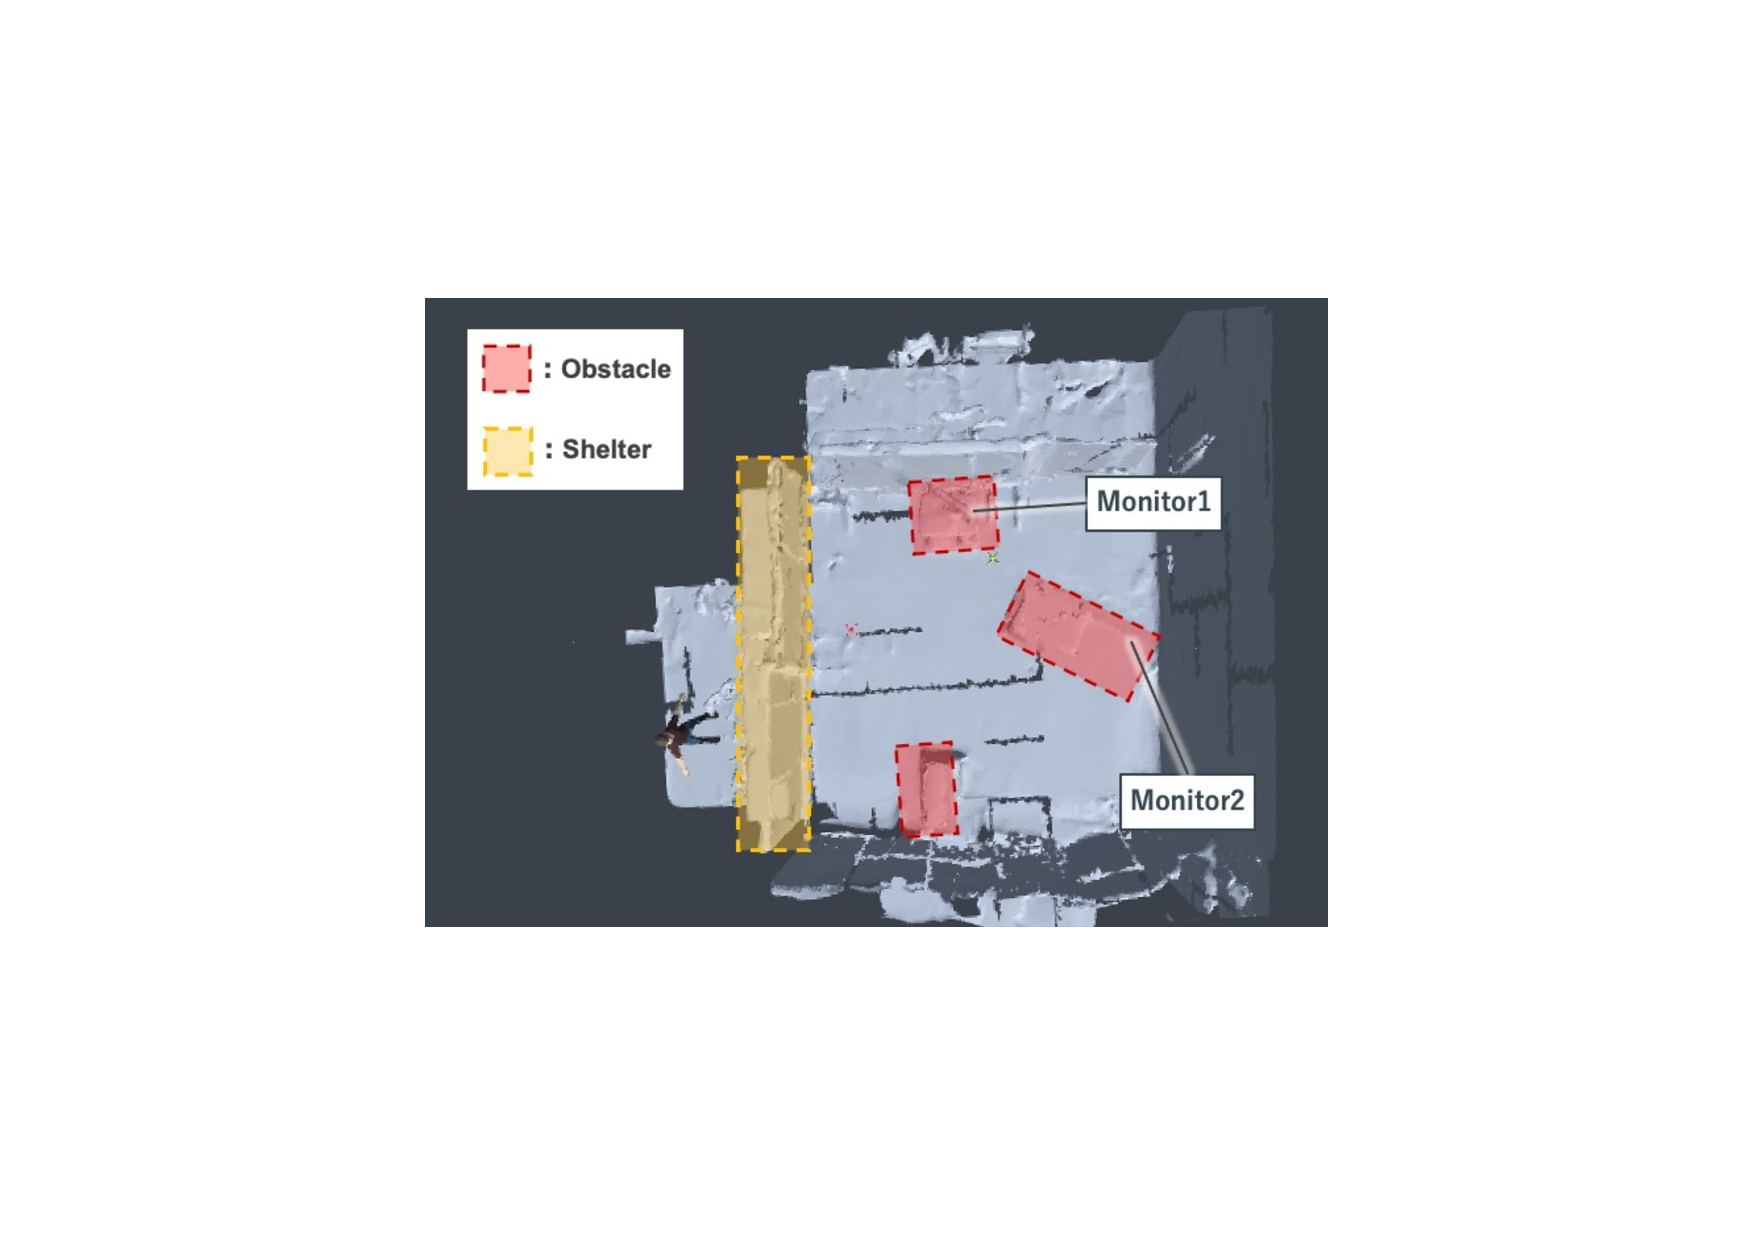
\includegraphics[width=0.7\linewidth]{img/05_experiment.pdf}
  \caption{実験環境}
  \label{fig:05_experiment}
\end{figure}

% \begin{figure}[!tb]
%   \centering
%   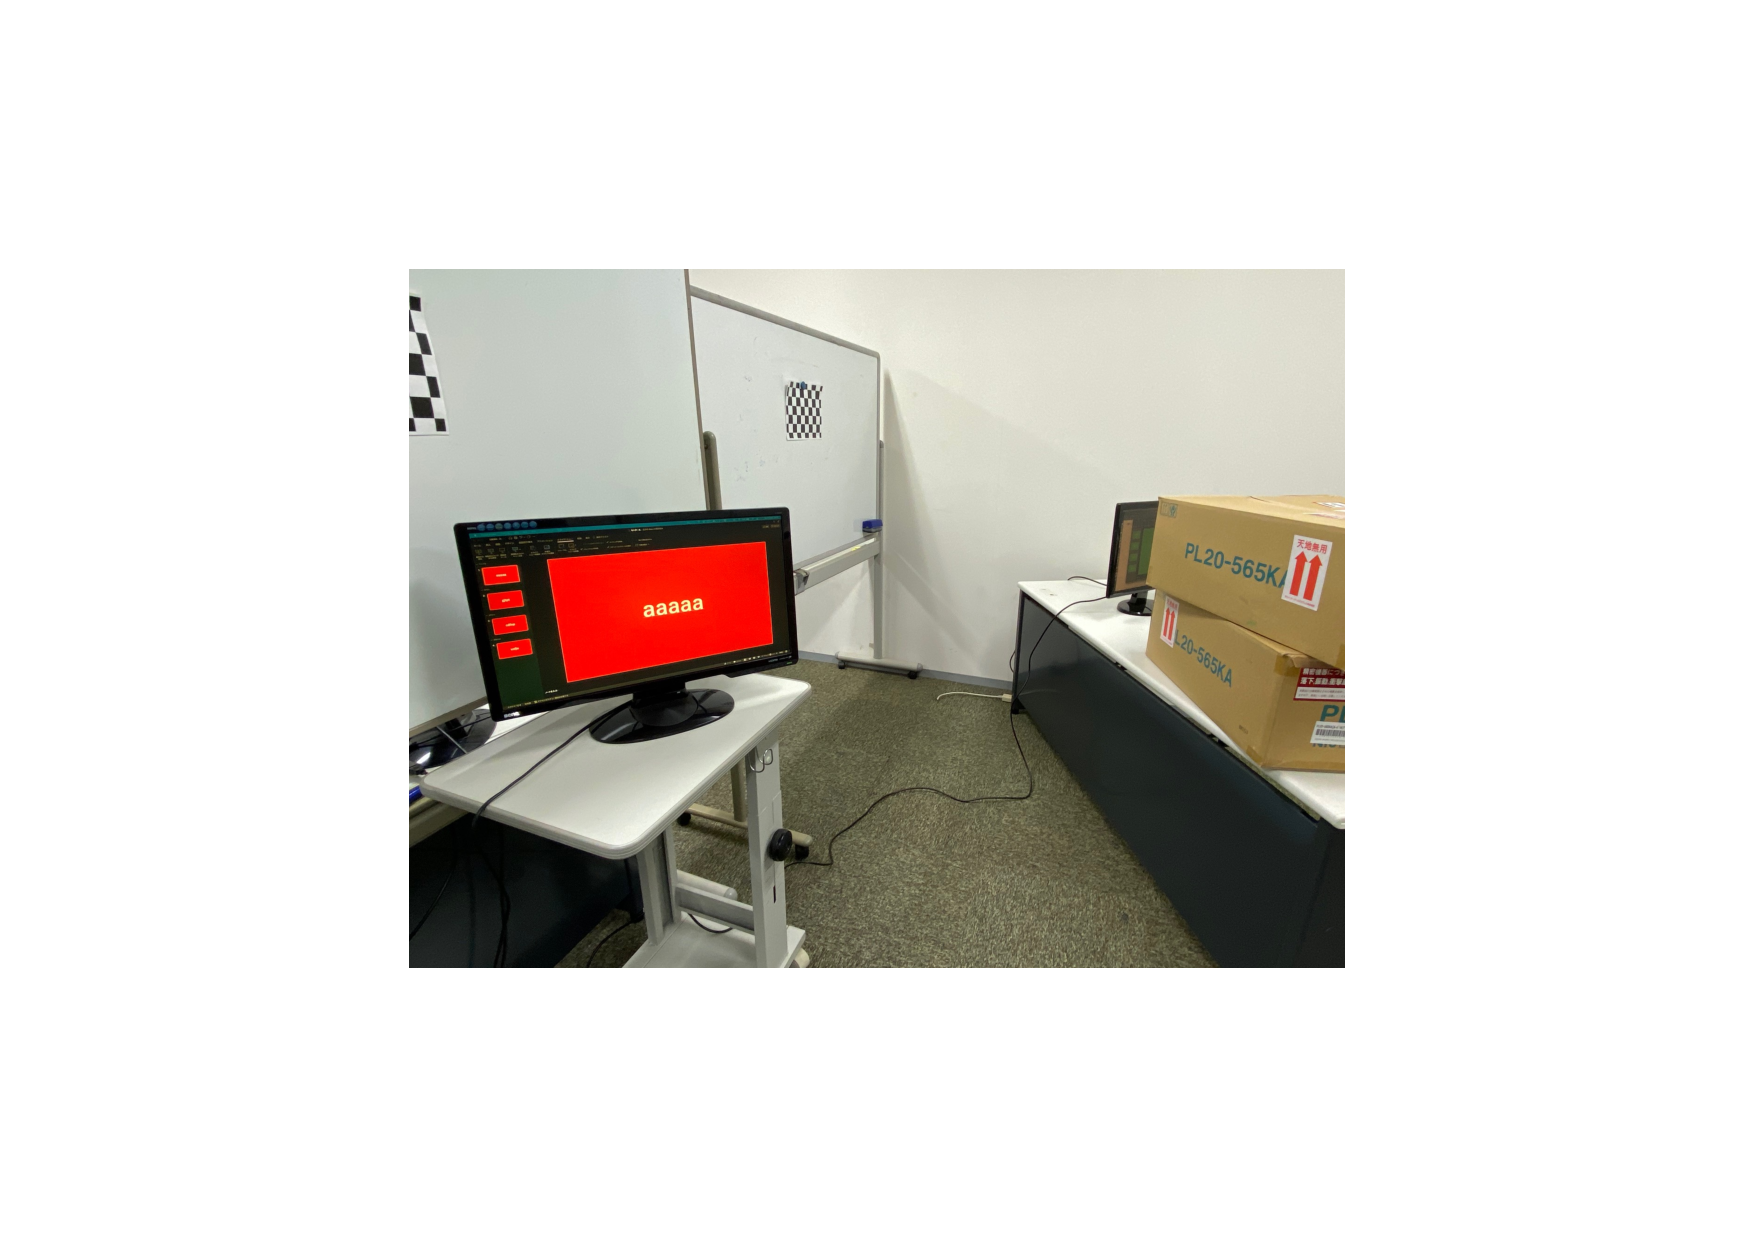
\includegraphics[width=0.7\linewidth]{img/05_monitor.pdf}
%   \caption{実験で使用するモニター}
%   \label{fig:05_monitor}
% \end{figure}

\par
また参加者へのアンケートでは,主観的な認識と好みを測定するために,1 〜 7 の7段階のリッカート尺度(1 = 全く同意しない,7 = 完全に同意する)のアンケートを実施した.
\par
アンケートでは,危険な障害物を判断できたか,状況把握の容易さの2項目を設けた.
実験の最後には,参加者にはどの方式が最も操縦性が良かったかを選択し,なぜその方式が良かったのか,また,なぜ他の方式を選択しなかったかという項目を設けた.
\par
タスク完了までの平均操縦時間,平均衝突警告回数にはrANOVA(反復測定分散分析,Repeated Measures ANOVA)を用いて統計解析した.
また,Post-hoc検定では,Bonferroni法を行い,各方式の比較を行なった.
アンケート結果では,Friedman検定を行い,Post-hoc検定ではBonferroni法を行い,各方式の比較を行なった.
    

% ******************** Section ********************
\section{評価実験}
\label{sec:Experiment}

死角領域内での未知領域探査におけるドローン操縦において,各方式がどのような影響を与えるかを評価するため,5人の実験協力者による実験を行なった.
参加者の平均年齢は23.8歳であり,ドローン操縦経験のある参加者が2名,ドローン操縦経験のない参加者が3名だった.
実験は約60分で行い,導入,各提案方式の練習,ARのキャリブレーション,タスク,アンケートの5つのフェーズから構成する.
\par
まず,参加者は本研究の概要と,操縦方法の説明を受け,その後,各方式の練習を行う.予備実験で,操縦の慣れによる実験後半の操縦時間短縮や,ARの経験がないことによる操縦時間増加を引き起こすことがわかった.
そのため,この効果を打ち消すために,ドローン操縦を5〜10分ほど練習した後に,各方式で実験環境を1度飛行することで,練習量を増やし,慣れによる差異を無くした.
\par
次にAR方式では,HoloLensアプリケーションを起動し,現実空間とのキャリブレーションを行い,参加者はHoloLensを装着した.
\par
その後,タスクを行い,各方式でタスクを完了する度に,実験を行なった方式についてアンケートを記入し,全方式を終了したら,どの方式が最も効果的であったかを選択し,その理由を記入してもらった.
また,なぜ他の方式を選択しなかったのか,その理由も記入してもらった.

% ******************** Section ********************
\section{評価結果}
\label{chap:Performance}

\begin{figure}[!b]
  \centering
  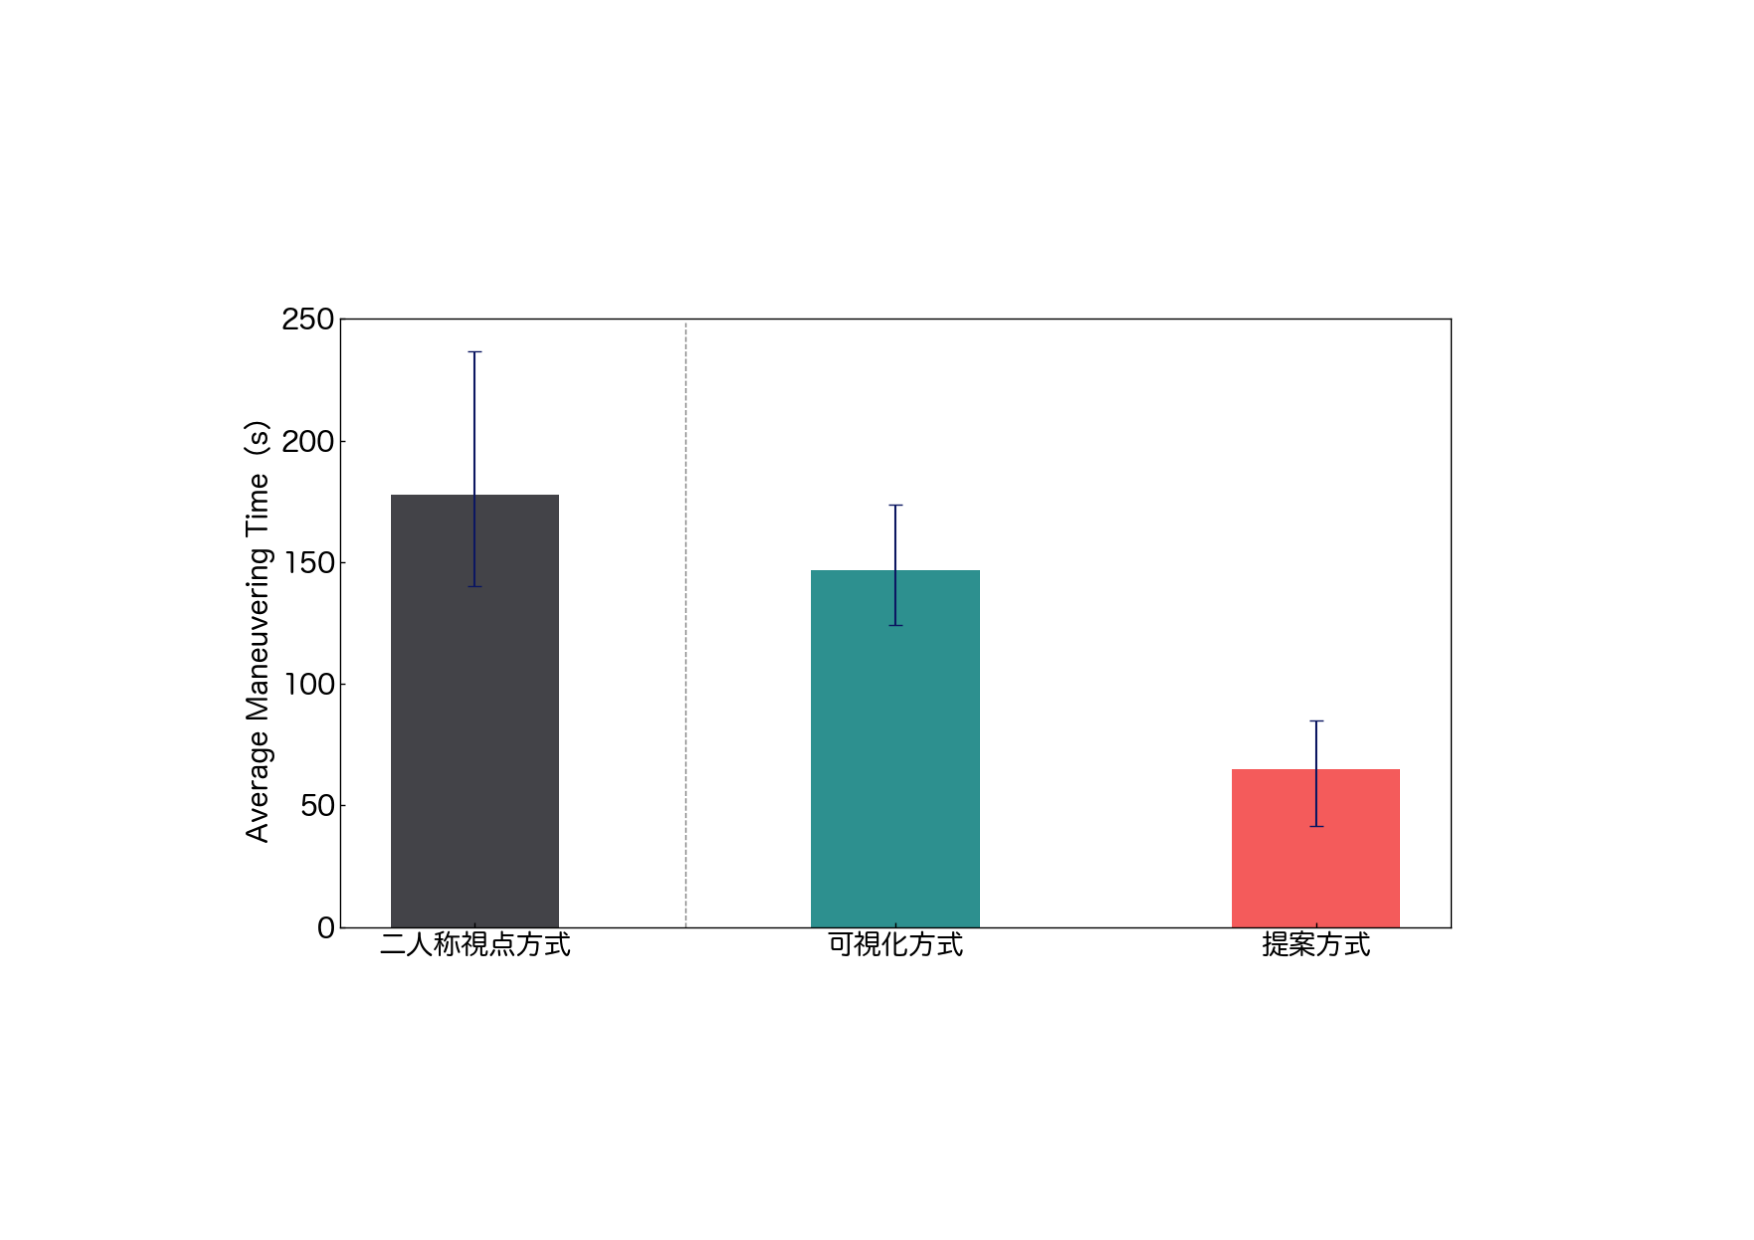
\includegraphics[width=0.7\linewidth]{img/05_time.pdf}
  \caption{平均操縦時間}
  \label{fig:05_time}
\end{figure}

\begin{figure}[!tb]
  \centering
  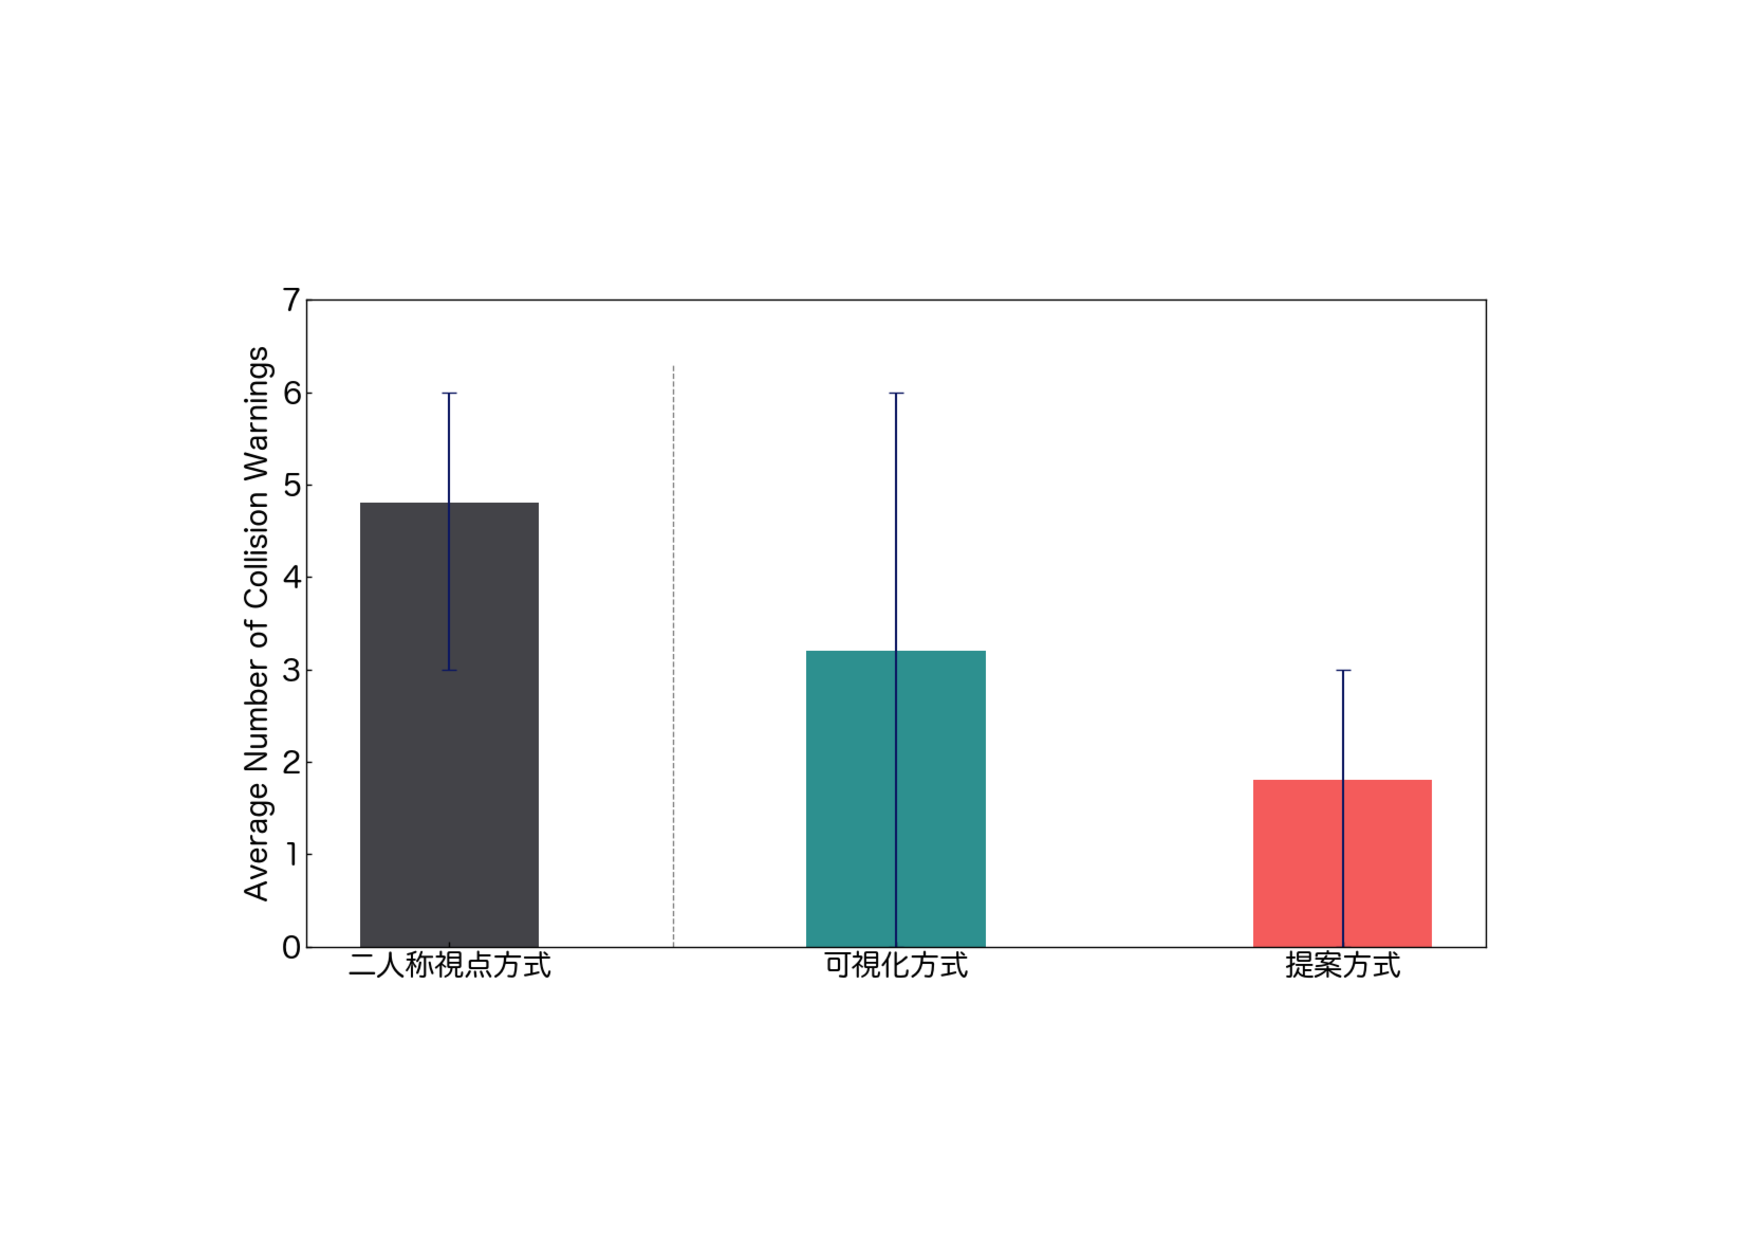
\includegraphics[width=0.7\linewidth]{img/05_collision.pdf}
  \caption{平均衝突警告回数}
  \label{fig:05_collision}
\end{figure}


\subsection{ドローン操縦の定量的評価}
\label{sec:QuantitativePerformance}

タスク完了までの平均操縦時間の評価結果を\figref{fig:05_time}に示す.
平均操縦時間では,rANOVAの結果,3方式の少なくともどれか一つに有意な差があった($F$ = 26.179, $p < 0.001 $).
Bonferroni法の多重比較($p < 0.05$)では,提案方式は二人称視点方式,可視化方式より,平均操縦時間は有意に減少することがわかった($p < 0.05$).
しかし,可視化方式は二人称視点方式と比較して,平均操縦時間が有意に減少しなかった($p = 0.201$).
% 距離画像方式では,従来の操縦手法である二人称視点方式の平均操縦時間と比較して約30\% 減少しているため,AR方式の中でも平均操縦時間を大いに削減している.
\par
次に,障害物への平均衝突警告回数の結果を\figref{fig:05_collision}に示す.
平均衝突警告回数では,rANOVAの結果,3方式の少なくともどれか一つに有意な差があった($F$ = 26.179, $p < 0.001 $).
Bonferroni法の多重比較($p < 0.05$)では,提案方式は二人称視点方式より,平均衝突警告回数は有意に減少することがわかった($p < 0.05$).
しかし,可視化方式は二人称視点方式と比較して,平均衝突警告回数が有意に減少しなかった($p = 0.3607$).
また,提案方式は可視化方式と比較して,平均衝突警告回数が有意に減少しなかった($p = 0.6169$).
\par
次に,ドローン操縦の不安度の結果を\figref{fig:05_command}に示す.
縦軸はタスク完了までにドローンへ移動命令を行なったコマンド総入力回数,横軸はドローンに移動命令を行なった際の各コマンドの時間間隔となっている.
二人称視点方式では,コマンド時間間隔が0〜2秒以内に集まっており,可視化方式は2〜3.5秒以内に集まっており,提案方式は0.5〜1.5秒以内に集まっている.

\begin{figure}[!b]
  \centering
  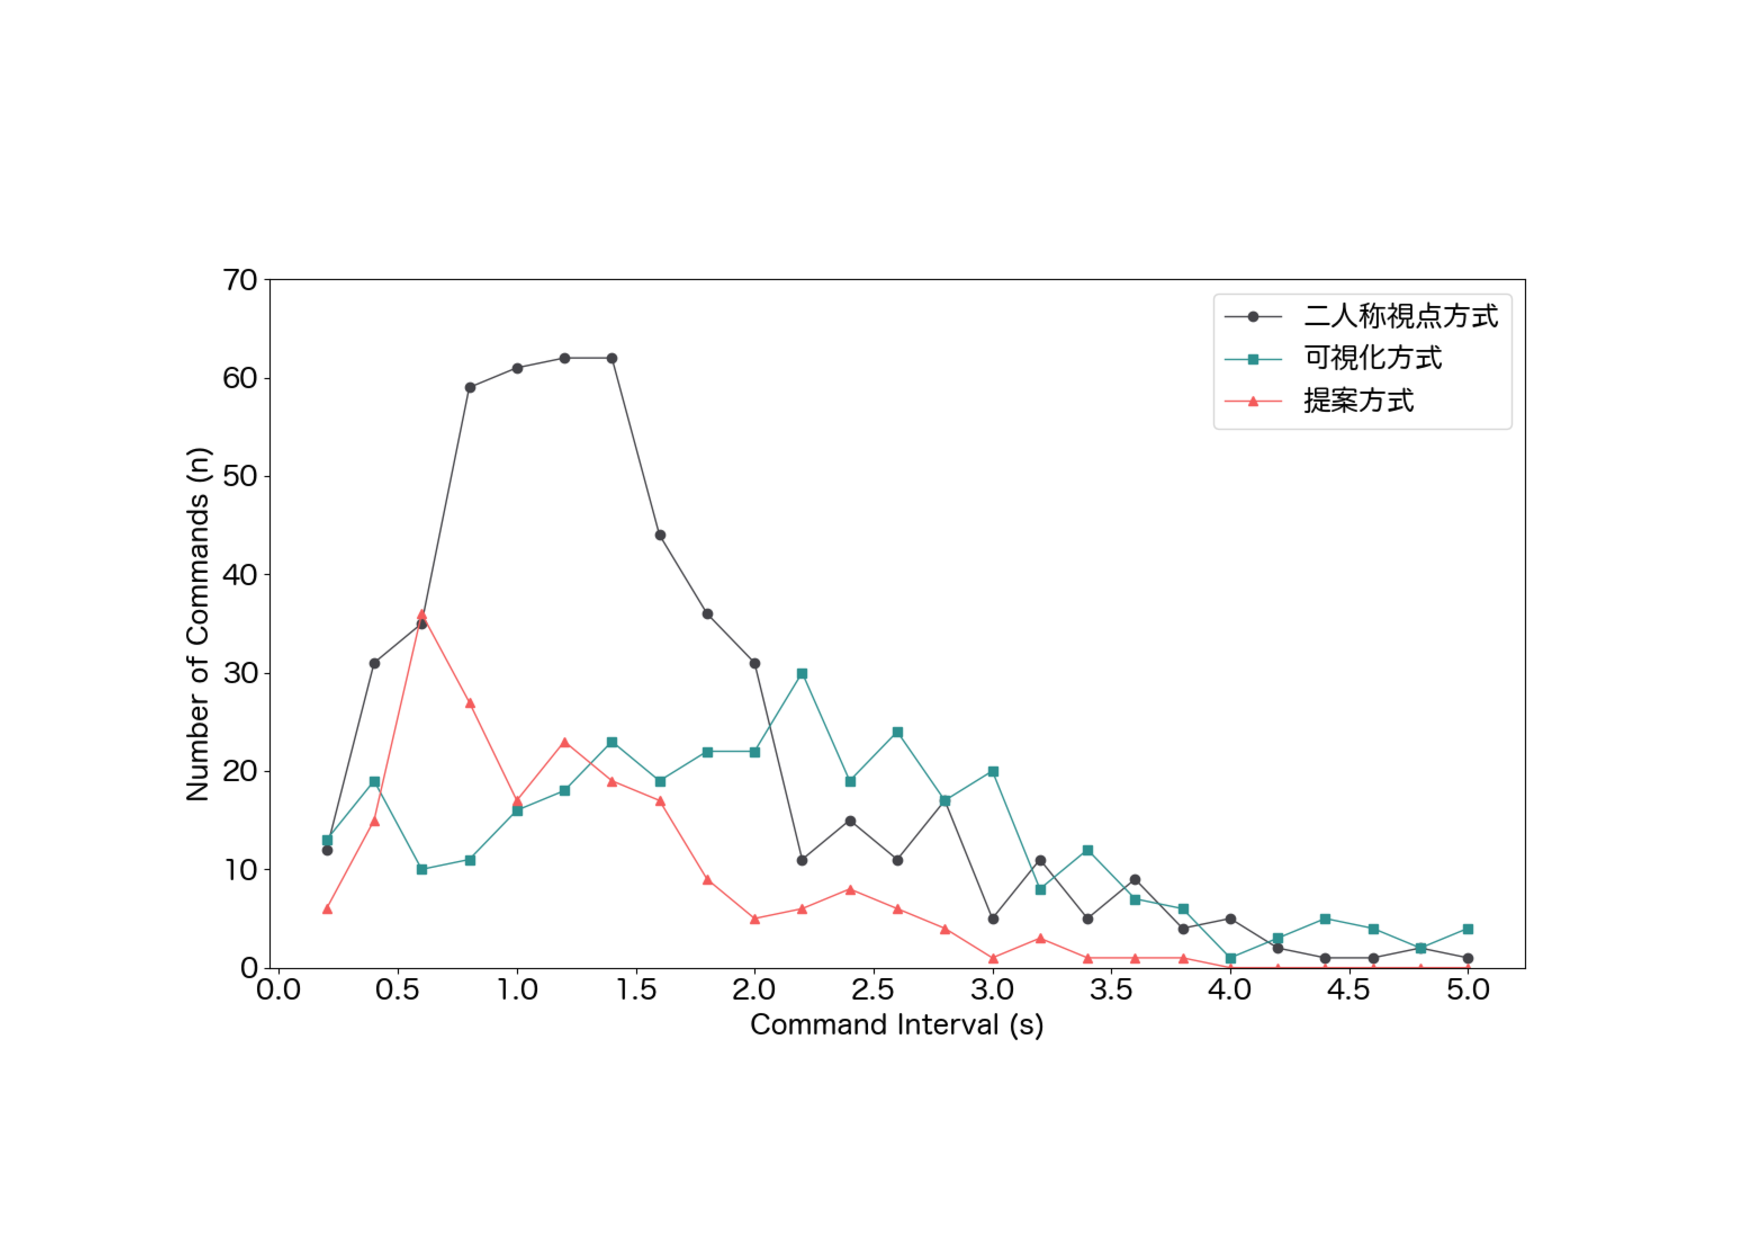
\includegraphics[width=0.7\linewidth]{img/05_command.pdf}
  \caption{ドローン操縦の不安度}
  \label{fig:05_command}
\end{figure}

% ******************** Section ********************
\subsection{ドローン操縦の定性的評価}
\label{sec:QualitativePerformance}


\begin{figure}[!b]
  \centering
  \begin{minipage}{0.45\linewidth}
    \centering
    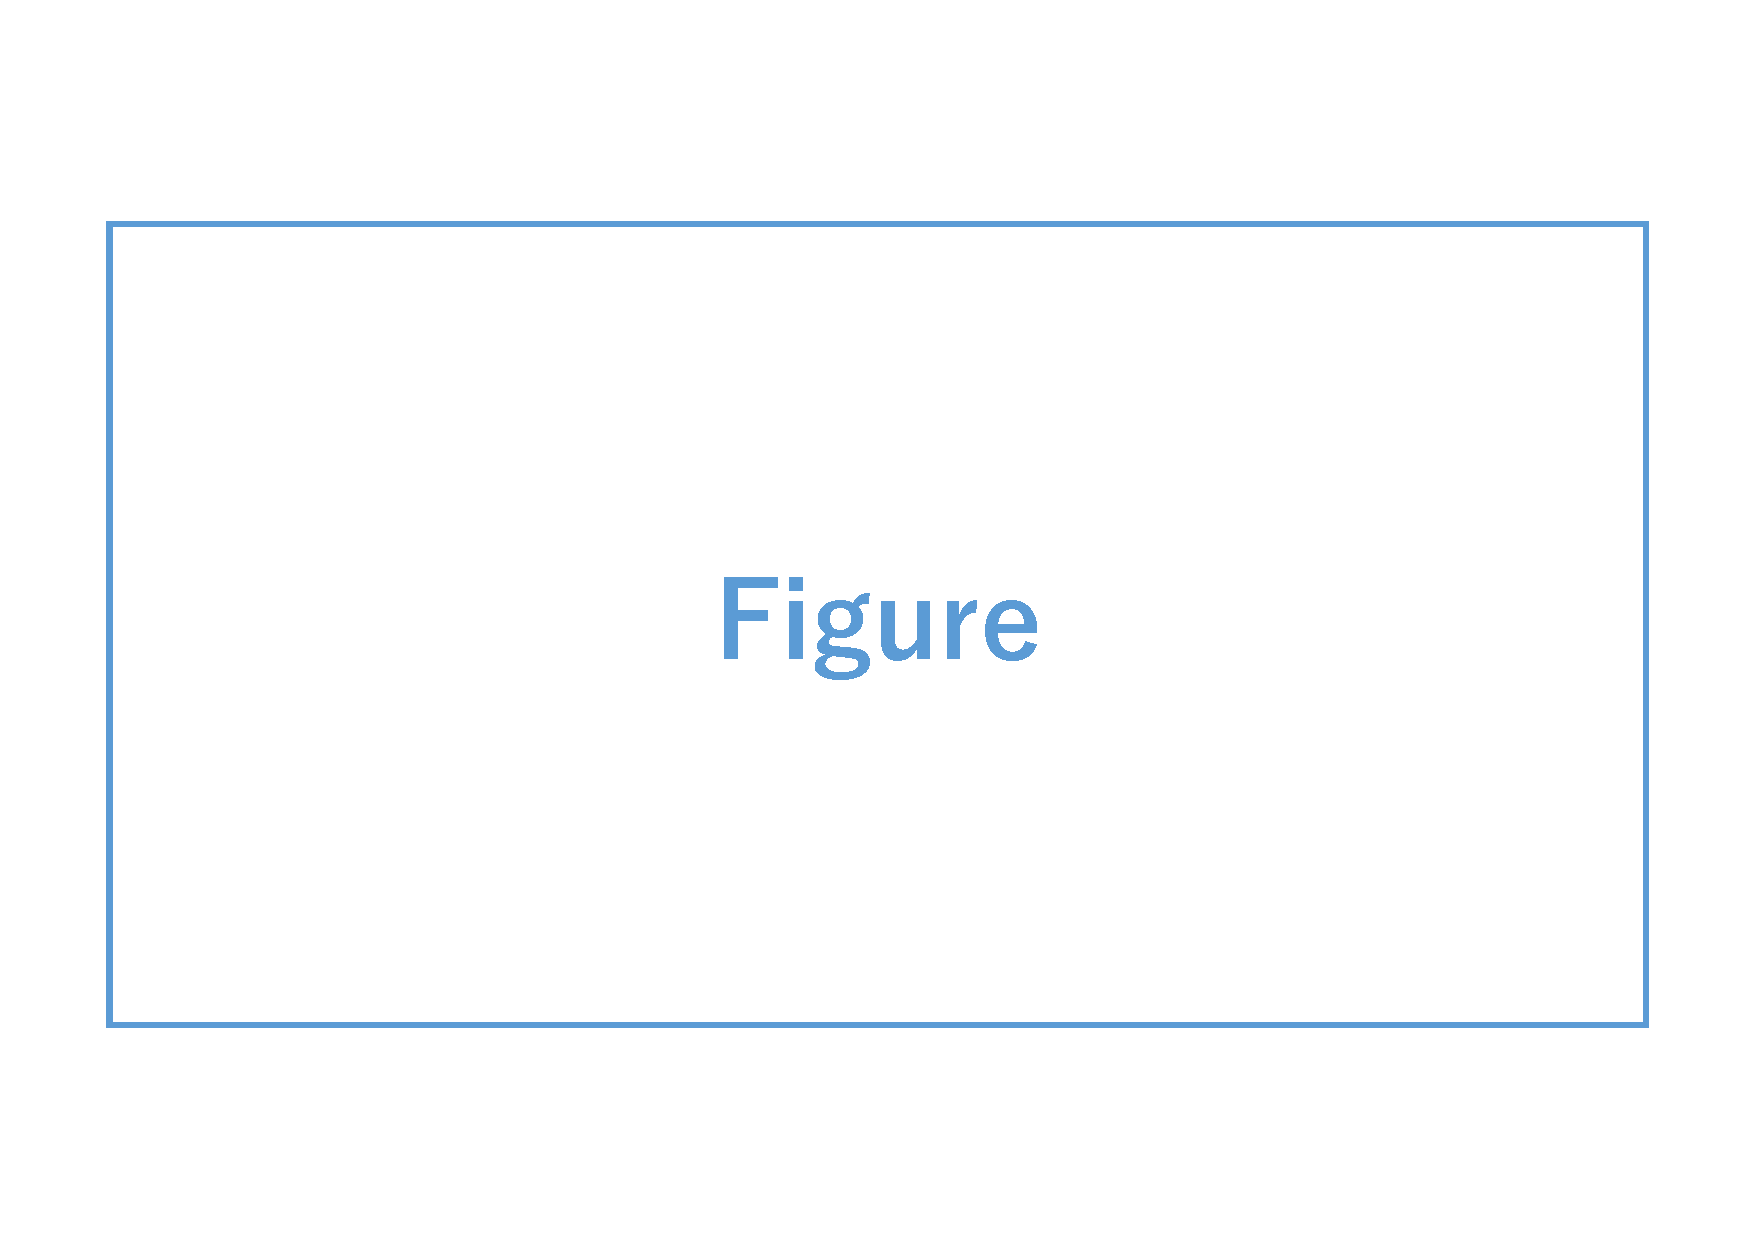
\includegraphics[width=0.95\linewidth]{img/sample.pdf}
    \caption{危険な障害物を判断できたか}
    \label{fig:05_likert1}
  \end{minipage}
  \begin{minipage}{0.45\linewidth}
    \centering
    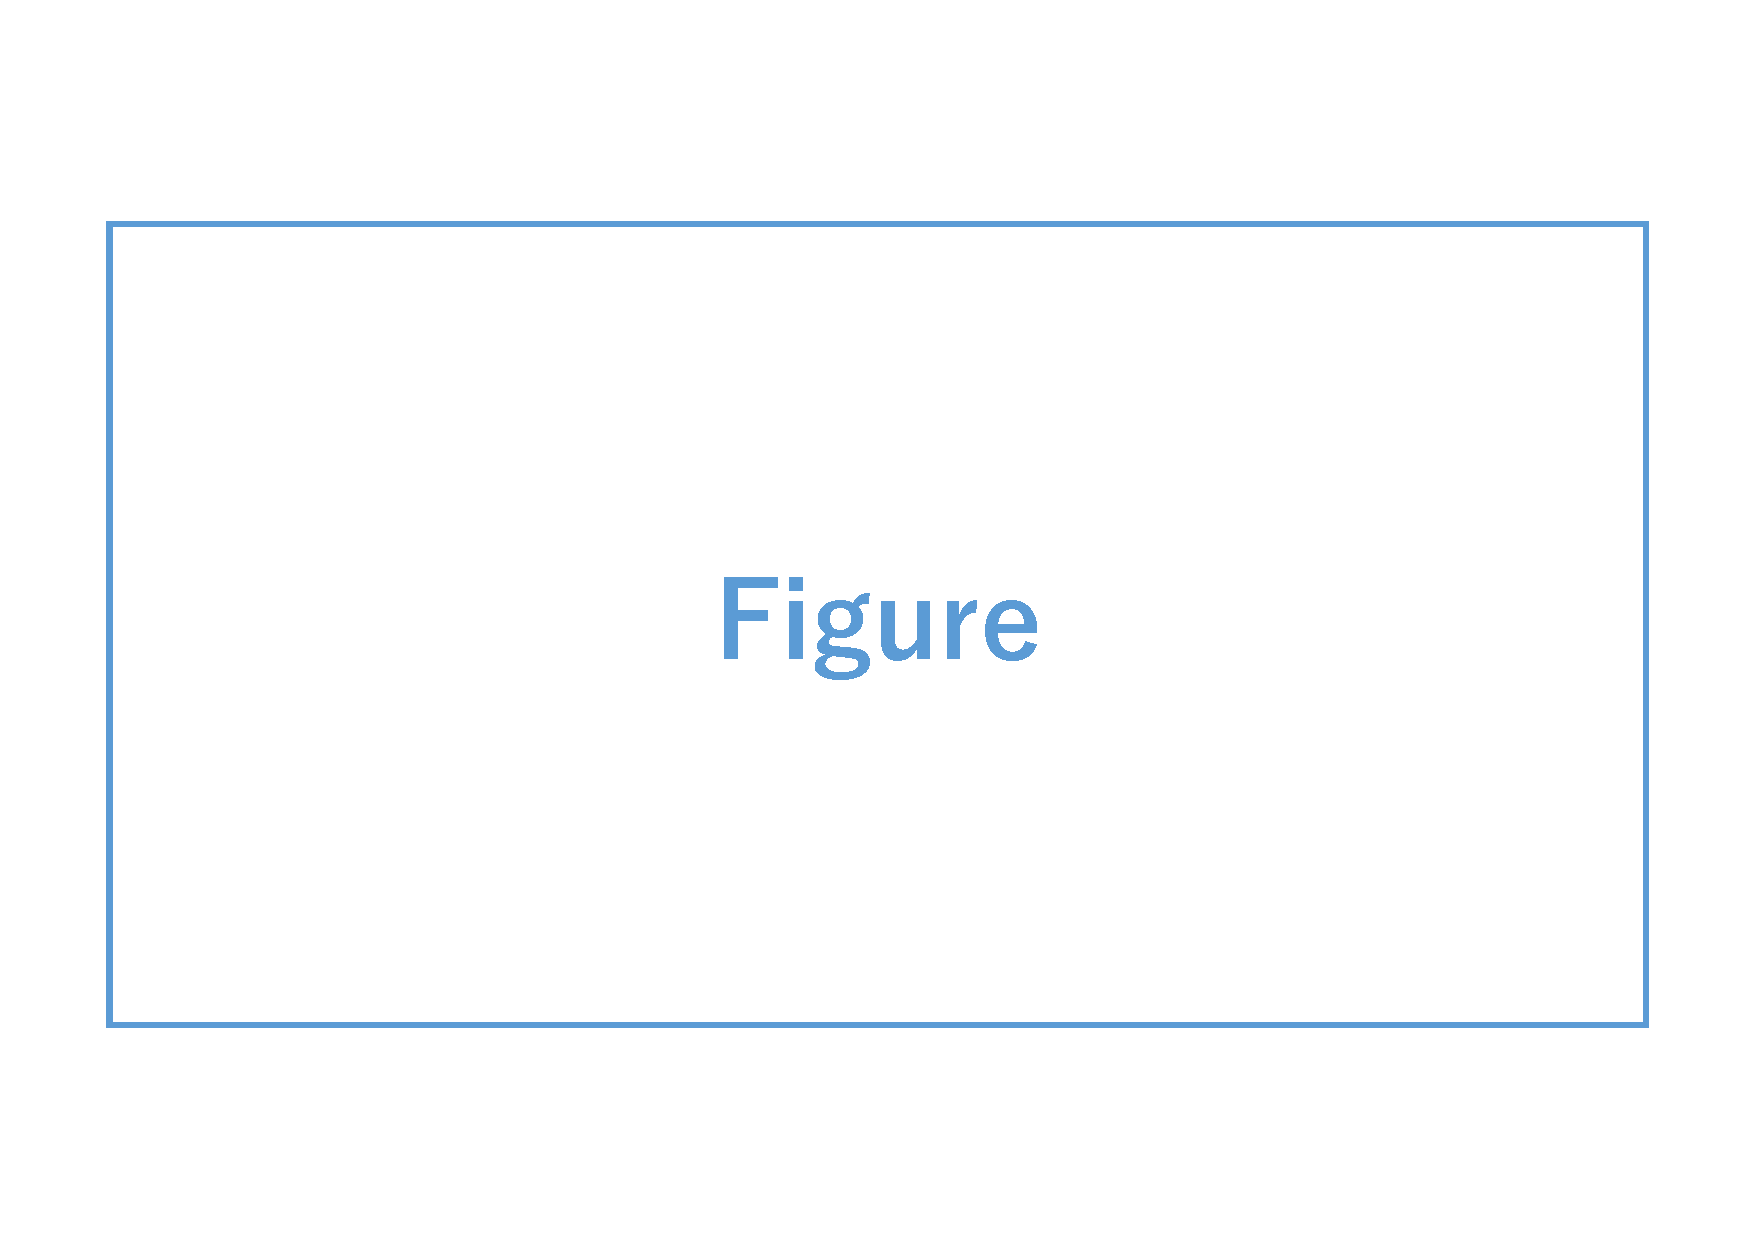
\includegraphics[width=0.95\linewidth]{img/sample.pdf}
    \caption{状況把握の容易さ}
    \label{fig:05_likert2}
  \end{minipage}
\end{figure}

% \label{sec:ScalabilityExperiment}

3つの各方式を比較するアンケート結果を\figref{fig:05_likert1},\figref{fig:05_likert2}に示す.
アンケート結果では,危険な障害物知覚($\chi^{2}(3)=27.875, p < 0.001$),状況把握の容易さ($\chi^{2}(3)=28.372, p < 0.001$)の2項目に対してFriedman検定を行ったところ,3方式の少なくともどれか一つに有意な差があった.
% それぞれの結果に対しBonferroni法の多重比較($p < 0.05$)を行ったところ,操縦の安心度では,距離画像方式,マーカー方式は二人称視点方式より,有意に向上した($p < 0.05$)が,可視化方式は二人称視点方式より有意に向上しなかった($p = 0.076$).
% また,マーカー方式は可視化方式より有意に向上しなかった($p = 0.251$)が,距離画像方式は可視化方式,マーカー方式より有意に向上したことがわかった($p < 0.05$).
% \par
% 危険な障害物を判断できたかを確認する項目では,距離画像方式,マーカー方式は二人称視点方式より有意に向上した($p < 0.05$)が,可視化方式は二人称視点方式より有意に向上しなかった($p = 0.124$).
% また,マーカー方式は可視化方式より有意に向上しなかった($p = 0.107$)が,距離画像方式は可視化方式,マーカー方式より有意に向上したことがわかった($p < 0.05$).
% \par
% 次に,ARを用いた方式のみを比較するアンケート結果を\figref{fig:04_likert3},\figref{fig:04_likert4}に示す.
% ARを用いた方式のみを比較するアンケート結果では,状況把握の容易さ($\chi^{2}(2)=18.667, p < 0.001$),操縦の自信度($\chi^{2}(2)=17.886, p < 0.001$)の2項目に対してFriedman検定を行ったところ,3方式の少なくともどれか一つに有意な差があった.
% それぞれの結果に対しBonferroni法の多重比較($p < 0.05$)を行ったところ,
% 状況把握の容易さでは,マーカー方式は可視化方式と比較し有意に向上しなかった($p = 0.091$)が,距離画像方式のみ可視化方式とマーカー方式と比較し有意に向上したことがわかった($p < 0.05$).
% \par
% 操縦の自信度でも同じく,マーカー方式は可視化方式と比較し有意に向上しなかった($p = 0.059$)が,距離画像方式のみ可視化方式とマーカー方式と比較し有意に向上したことがわかった($p < 0.05$).


%----------------------------------------------------------------------
% 考察
%----------------------------------------------------------------------
\chapter{考察}
\label{chap:Discussion}

ここでは,\ref{chap:Experiment}章で述べた評価結果をもとに考察を行う.
ドローンが撮影する映像を頼りに操縦を行う従来のドローン操縦手法である二人称視点方式と,ARを用いて操縦するドローンのカメラ映像を投影した上で死角領域内の空間認識を提供する可視化方式,複数ドローンのセンサ情報を統合した上でARを用いた死角領域内の空間認識を提供する提案方式を比較し分析を行う.

% ******************** Section ********************
\section{未知領域探査における効率性}
\label{sec:Efficiency}

本節では,各方式の評価結果について考察し,提案方式が死角領域内での未知領域探査におけるドローンの探査効率へ与える影響を考察する.
\par
平均操縦時間は\figref{fig:05_time}に示したように,提案方式は他方式と比較し,有意に減少した.
実験の様子から,二人称視点方式では,周囲に何があるか分からないため,確認する動作が他方式に比べ多くなっていた.
その上,自身が操縦するドローンとは別に,もう一台ドローンが飛行しているため,カメラに写っている範囲外へ進むことへ抵抗があり,周辺環境の確認に時間がかかっていた.
また,可視化方式ではドローンのカメラ映像をもとに三次元環境地図を復元するため,二人称視点方式と同様にドローンに周辺を確認させる作業を行う必要があり,
操縦時間を大幅に減少できなかったと推測される.
一方で,提案方式では実験環境に飛行しているもう一台のドローンのセンサ情報を統合しているため,もう一台のドローンのカメラ映像も使用し三次元環境地図を復元しており,
ドローン周辺を見渡す機会が少なく,操縦時間を有意に減少させていたと考察できる.
\par
\figref{fig:05_command}に示したドローン操縦の不安度では,可視化方式のみコマンド間隔時間が長かった.
二人称視点方式と提案方式では,コマンド間隔時間が短いため,ドローン操縦への不安度は少ないように推測できるが,二人称視点方式ではコマンド数が60回程度まで増加しているため,
ドローン操縦での無駄な動作多いことがわかる.
そのため,二人称視点方式はコマンド間隔時間は短いが,コマンド総入力回数が多いことより,ドローン操縦の不安度が高いことがわかる.
可視化方式では,コマンド総入力回数が二人称視点方式より少ないが,コマンド間隔時間が平均的に長いことがわかる.
実験の様子から,ドローンを連続で移動させることは珍しく,慎重に操縦している傾向があった.
そのため,可視化方式ではARによる空間認識に加え,ドローンのカメラ映像もあることにより,他の方式に比べ操縦者に与えられる情報量が多く,
ドローン操縦に躊躇いが生じていると考察できる.
一方で,提案方式はドローン周辺の環境の復元が速いため,状況を把握するのに必要な時間と操作数が最も少なく,どちらに進めればいいかが明確であった.
そのため,一回のドローン操縦で長い距離を走行し,短時間に,短いコマンド間隔時間で実験を進めていることを確認した.

以上より,提案方式は他の方式と比較して,操縦者のドローン操縦への自信度を最も向上させており,タスク完了までの平均操縦時間も有意に減少しているため,
複数ドローンが混在する未知領域探査において,探査効率を向上したことを確認した.


% ******************** Section ********************
\section{未知領域探査における安全性}
\label{sec:Safety}

本節では,各方式の評価結果について考察し,提案方式が死角領域内での未知領域探査におけるドローン操縦の安全性へ与える影響を考察する.
\par
平均衝突警告回数は\figref{fig:05_collision}に示したように,提案方式は二人称視点方式と比較し,有意に減少した.
これは,死角領域内を可視化することによって,ドローン周辺に何があるか把握することができるためだと推測できる.
しかし,提案方式は可視化方式と比較し,有意に減少しなかった.
実験参加者の自由回答では,可視化方式より与えられる安心感を指摘する意見が多かった.
そのため,可視化方式はドローン周辺の三次元環境地図を復元することには時間がかかるが,カメラ映像があるため,安心してドローン操縦を行えていると推測できる.
その一方で,提案方式では自身が操縦するドローンとは別のドローンの位置を把握でき,その上,遮蔽物の危険度を可視化していたため,操縦者へ安心感を与えることはできていた.
しかし,遮蔽物のみの危険度を可視化していたため,操縦者が気になる障害物が危険な位置にあるか把握できない可能性があり,
提案方式は可視化方式より有意に減少しなかったと考察できる.

以上より,可視化方式,提案方式は従来操縦である二人称視点方式よりドローン操縦の安全性を向上させることができる.
しかし,未知領域探査における一人称視点でのドローン操縦では,死角領域内のAR可視化が有効ではあるが,
複数ドローンが混在する環境下では,操縦者とドローン間に位置する遮蔽物の危険度を提供するだけでは不十分であることがわかった.
提案方式では,複数ドローンのセンサ情報を統合することにより,未知領域探査効率は向上させることができるが,
安全性をより向上するためには,常にドローン周辺の危険性を示す,周辺環境の全体的な理解と安心感を提供する必要があることを確認した.





%----------------------------------------------------------------------
% おわりに
%----------------------------------------------------------------------
\chapter{おわりに}
\label{chap:Conclusion}

小型ドローンは機体の大きさを活かして,インフラ点検や災害調査のような,人間が立ち入れない狭小空間での活躍が増えており,将来的には狭小空間の未知領域探査への応用が期待されている.
しかし,狭小空間でのドローン飛行では,遮蔽物により視点が遮られる,死角領域内での操縦を必要とする.
また,従来の操縦手法では状況認識が不十分であるため,ドローン周辺に位置する障害物が多い狭小空間では,ドローン操縦は困難である.
そのため,遮蔽物,障害物が多い狭小空間では,死角領域内におけるドローン飛行の危険性を軽減する必要がある.

また,狭小空間の未知領域探査では,走行する環境情報がなく,一台のドローンのみで探査を行うには多くの時間を必要とするため,バッテリー上限が短いドローンでは,探査を完了することが困難である.
そこで,複数台のドローンを使用することで,各ドローンの走行時間を減少させ,探査効率を向上させることを期待されている.
しかし,ドローンの数が多いほど衝突のリスクは高く,また,探査領域の重複による探査効率の低下を招く可能性がある.

そこで本研究では,各ドローンがリアルタイムで取得する位置情報,三次元環境地図のセンサ情報を統合し,ARを用いて操縦者の死角領域内に存在するドローンと周辺環境を可視化する方式を提案する.
本提案方式について,死角領域内での未知領域探査におけるドローン操縦の安全性,探査の効率性,ドローン操縦の不安度を評価実験する.

結果として,提案方式では実験環境での平均操縦時間が短く,ドローン操縦の不安度も少なかったことから,未知領域探査での探査効率の向上を示した.
また,平均衝突警告回数は従来操縦と比較し少なかったため,狭小空間による死角領域内のドローン安全性向上を示した.\\

\clearpage

%----------------------------------------------------------------------
% 謝辞
%----------------------------------------------------------------------
\chapter*{謝辞}
\addcontentsline{toc}{chapter}{謝辞}  % 章番号のない章を目次に表示させる
\label{chap:Acknowledgments}

本研究を進めるにあたって,多大なご指導とご支援を賜りました同志社大学理工学部の佐藤健哉
教授に心より感謝致します.また,3年間研究生活を共に過ごし,研究に就職活動と共に乗り越えた
ネットワーク情報システム研究室の同期,研究・就職活動の相談に乗ってくださった先輩,研究室生
活で慕ってくれた後輩,さらに様々な場面で支えてくれた家族と友人へ感謝します.
\clearpage

%----------------------------------------------------------------------
% 付録
%----------------------------------------------------------------------
% \appendix
% \chapter{ソースコード}
% \label{chap:apndx:src}

%----------------------------------------------------------------------
% 参考文献
%----------------------------------------------------------------------
\renewcommand{\bibname}{参考文献}

\addcontentsline{toc}{chapter}{参考文献}  % 章番号のない章を目次に表示させる

% thebibliography を利用する場合は以下を使用(拘りがなければこちらでOK)
% \begin{thebibliography}{99}
%   \bibitem{LaTexWiki} Latex Wiki. \url{https://texwiki.texjp.org/}.
%   \bibitem{渡辺豊2016} 渡辺 豊, "角皆静男先生のご逝去を悼む", 地球化学, vol.50, no.1, pp.1-3, 2016.
% \end{thebibliography}

% BibTex を利用する場合は以下を使用(初めての人には難しいかも)
\bibliographystyle{junsrt}
\bibliography{myref}

\clearpage

%----------------------------------------------------------------------
% 研究業績
%----------------------------------------------------------------------
\renewcommand{\bibname}{研究業績}

\addcontentsline{toc}{chapter}{研究業績}

\begin{thebibliography}{99}
  \bibitem{} 竹内 一真, 滕 睿, 佐藤 健哉, [推薦論文]狭小空間監視のためのドローンを利用したAR可視化方式の実装と評価, 情報処理学会論文誌, 2022.(採録決定).
  \bibitem{} 竹内 一真, 滕 睿, 佐藤 健哉, 狭小空間監視のためのドローンを利用したAR可視化手法の実装と評価, 情報処理学会研究報告, Vol.2022-ITS-88, No.7, pp.1-8, 2022/3.(優秀論文賞受賞).
  \bibitem{} 竹内 一真,林 聡一郎,上原 夏紀,佐藤 健哉,3次元環境認識に基づく死角領域内のAR可視化によるドローン操縦性向上,情報処理学会第83回全国大会論文集, Vol.3, pp.345-346, 2021/3.
  \bibitem{} 鈴木 彩門, 竹内 一真, 滕 睿, 佐藤 健哉, 複数人によるAR空間文字情報共有時の向き補正手法, 情報処理学会第84回全国大会論文集, Vol.3, pp.187-188, 2022/3.
  \bibitem{} 松下 翔太, 土居 大輝, 竹内 一真, 滕 睿, 佐藤 健哉, 移動環境におけるビデオストリーミング品質向上のためのMPQUICスケジューラの検討, 情報処理学会第85回全国大会論文集, 2022/3.(発表予定)
\end{thebibliography}

\clearpage

%----------------------------------------------------------------------
\end{document}
%----------------------------------------------------------------------
